\documentclass[11pt,a4paper]{article}
\usepackage[utf8]{inputenc}
\usepackage[spanish]{babel}	%Idioma
\usepackage{amsmath}
\usepackage{amsfonts}
\usepackage{amssymb}
\usepackage{graphicx} 	%Añadir imágenes
\usepackage{geometry}	%Ajustar márgenes
\usepackage[export]{adjustbox}[2011/08/13]
\usepackage{float}
\restylefloat{table}

\usepackage{titling}
%\usepackage{minted}
\usepackage{multirow}
\usepackage{caption}
\usepackage{multicol}
\usepackage[shortlabels]{enumitem}
\usepackage{array}
\selectlanguage{spanish}
\PassOptionsToPackage{hyphens}{url}\usepackage[hidelinks]{hyperref}

%Paquetes gráficos
\usepackage{tikz}
\usetikzlibrary{matrix,calc}

%Opciones de encabezado y pie de página:
\usepackage{fancyhdr}
\pagestyle{fancy}
\lhead{Nazaret Román Guerrero}
\rhead{Sistemas Multimedia}
\lfoot{Grado en Ingeniería Informática}
\cfoot{}
\rfoot{\thepage}
\renewcommand{\headrulewidth}{0.4pt}
\renewcommand{\footrulewidth}{0.4pt}

%Opciones de fuente:
\usepackage[utf8]{inputenc}
\usepackage[default]{sourcesanspro}
\usepackage{sourcecodepro}
\usepackage[T1]{fontenc}

\setlength{\parindent}{15pt}
\setlength{\headheight}{15pt}
\setlength{\voffset}{10mm}

% Custom colors
\usepackage{color}
\definecolor{deepblue}{rgb}{0,0,0.5}
\definecolor{deepred}{rgb}{0.6,0,0}
\definecolor{deepgreen}{rgb}{0,0.5,0}

%Códigos fuente
\usepackage{listings}
\usepackage{color}
\usepackage{graphicx}

\definecolor{mygreen}{rgb}{0,0.6,0}
\definecolor{mygray}{rgb}{0.5,0.5,0.5}
\definecolor{mymauve}{rgb}{0.58,0,0.82}

\lstset{ 
  backgroundcolor=\color{white},   % choose the background color
  basicstyle=\footnotesize,        % the size of the fonts that are used for the code
  breakatwhitespace=false,         % sets if automatic breaks should only happen at whitespace
  breaklines=true,                 % sets automatic line breaking
  captionpos=b,                    % sets the caption-position to bottom
  commentstyle=\color{mygreen},    % comment style
  deletekeywords={...},            % if you want to delete keywords from the given language
  escapeinside={\%*}{*)},          % if you want to add LaTeX within your code
  extendedchars=true,              % lets you use non-ASCII characters; for 8-bits encodings only, does not work with UTF-8
  frame=single,	                   % adds a frame around the code
  keepspaces=true,                 % keeps spaces in text, useful for keeping indentation of code (possibly needs columns=flexible)
  keywordstyle=\color{blue},       % keyword style
  language=C,                 	   % the language of the code
  morekeywords={*,private},        % add more keywords to the set
  numbers=left,                    % where to put the line-numbers (none, left, right)
  numbersep=5pt,                   % how far the line-numbers are from the code
  numberstyle=\tiny\color{mygray}, % the style that is used for the line-numbers
  rulecolor=\color{black},         % if not set, the frame-color may be changed on line-breaks within not-black text
  showspaces=false,                % show spaces everywhere adding particular underscores; it overrides 'showstringspaces'
  showstringspaces=false,          % underline spaces within strings only
  showtabs=false,                  % show tabs within strings adding particular underscores
  stepnumber=1,                    % the step between two line-numbers. If 1, each line si numbered
  stringstyle=\color{magenta},     % string literal style
  tabsize=2,	                   % sets default tabsize to 2 spaces
  title=\lstname                   % show the filename of files included with \lstinputlisting; also try caption instead of title
}

\begin{document}
\begin{titlepage}

\begin{minipage}{\textwidth}

\centering

\includegraphics[width=0.5\textwidth]{logo.png}\\

\textsc{\Large Sistemas Multimedia\\[0.2cm]}
\textsc{GRADO EN INGENIERÍA INFORMÁTICA}\\[1cm]

{\huge \bfseries Manual de usuario\\}
\noindent\rule[-1ex]{\textwidth}{3pt}\\[3.5ex]
{\large\bfseries SMM 2018/2019}
\end{minipage}

\vspace{1.5cm}
\begin{minipage}{\textwidth}
\centering

\textbf{Autora}\\ {Nazaret Román Guerrero}\\[2.5ex]

\includegraphics[width=0.3\textwidth]{etsiit.jpeg}\\[0.1cm]
\vspace{1cm}
\textsc{Escuela Técnica Superior de Ingenierías Informática y de Telecomunicación}\\
\vspace{1cm}
\textsc{Curso 2018-2019}
\end{minipage}
\end{titlepage}

\pagenumbering{gobble}
\pagenumbering{arabic}
\tableofcontents
\thispagestyle{empty}

\newpage

\section{Ventanas internas}

\subsection{Análisis de requisitos}
Para poder gestionar gráficos, imágenes y vídeo en la misma aplicación, debe existir una jerarquía de ventanas internas que se encarguen de las distintas partes:

\begin{itemize}
	\item RF1. Ventana interna encargada de la gestión de gráficos.
	\item RF2. Ventana interna encargada de la gestión de imágenes y gráficos.
	\item RF3. Ventana interna encargada de la gestión de la webcam del dispositivo.
	\item RF4. Ventana interna encargada de la gestión de reproducción de vídeo.
\end{itemize}

\subsection{Explicación de cada requisito}
Para cada uno de los requisitos anteriores, se pide:

\begin{itemize}
	\item RF1. Se abrirá una ventana interna que gestione los gráficos, manteniendo todas las figuras en el lienzo, y cada una con sus propiedades.
	\item RF2. Se abrirá una ventana interna que gestione el procesamiento de imágenes y además, gráficos, manteniendo todas las figuras en el lienzo, cada una con sus propiedades.
	\item RF3. Se abrirá una ventana interna que gestione la cámara del dispositivo y que mostrará en tiempo real lo que capte la webcam.
	\item RF4. Se abrirá una ventana interna que gestione el vídeo, reproduciendo el que el usuario elija.
\end{itemize}

\subsection{Codificación}
Para que esto haya sido posible, se ha creado una jerarquía de ventanas internas que se puede observar en el siguiente diagrama de clases:

\begin{figure}[H]
\centering
	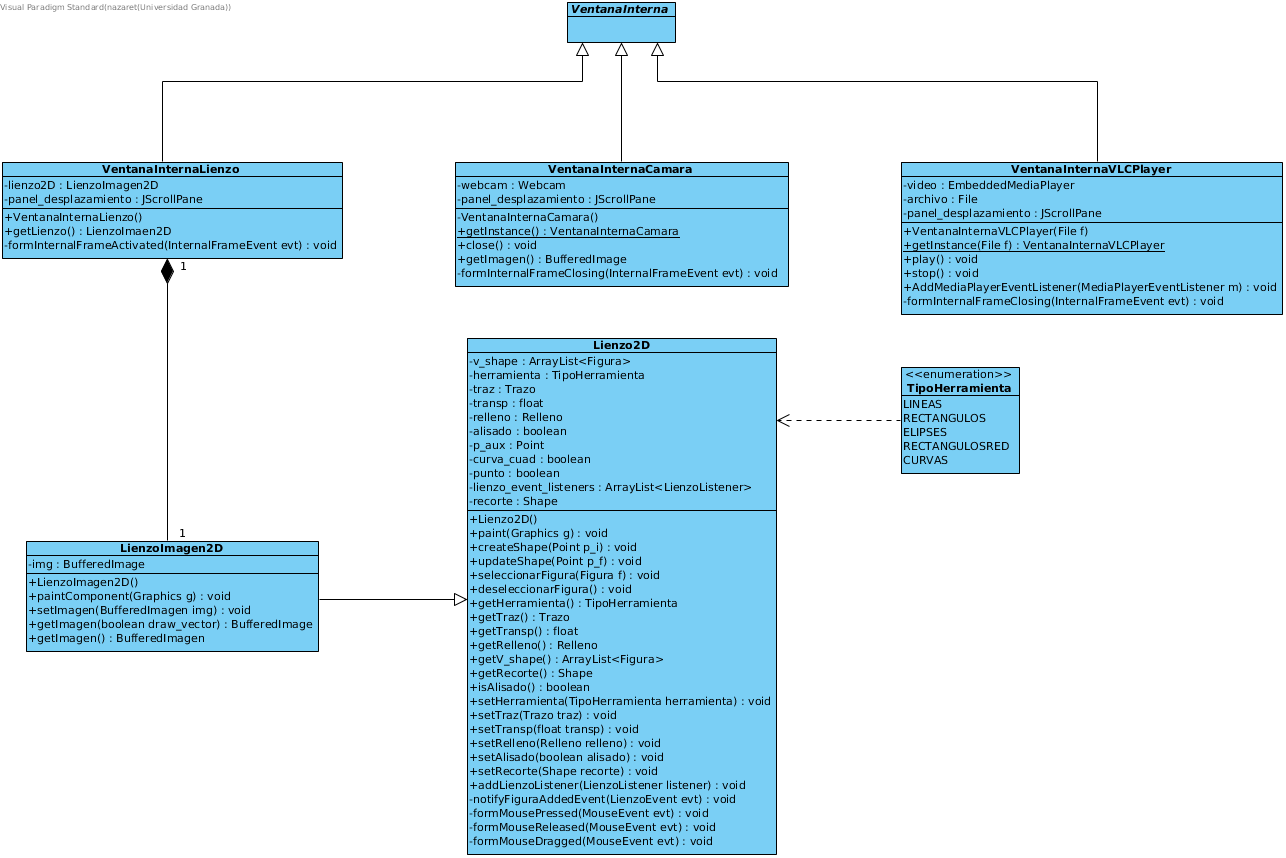
\includegraphics[scale=0.45]{./UML/vi.png}
\end{figure}

Como se puede observar, existe una superclase abstracta, \textsc{\textit{VentanaInterna}}, de la cual heredan las demás. Esta clase solo se utiliza para hacer el casting correspondiente y evitar errores en el código.\\ 

La \textsc{VentanaInternaCamara} es la encargada de ejecutar la webcam; la clase \textsc{VentanaInternaVLCPlayer} es la encargada de ejecutar el vídeo; y por último, la clase \textsc{VentanaInternaLienzo} es la encargada de gestionar gráficos e imagen. Para ello, la clase tiene un atributo de tipo \textsc{LienzoImagen2D} que permite el procesado de imágenes; ésta a su vez hereda de \textsc{Lienzo2D}, capaz de gestionar los gráficos creados por el usuario en el lienzo.\\

Este diagrama será incluido con el nombre de \textsc{VI.png} para que sea más legible puesto que en el documento puede ser difícil de leer.

\newpage

\section{Gráficos}

\subsection{Análisis de requisitos}
En lo referente a gráficos, la aplicación debe ser capaz de:

\begin{itemize}
	\item RF1. El lienzo mantendrá todas las figura a medida que se dibujen.
	\item RF2. Cada figura tendrá sus propios atributos:
		\begin{itemize}
			\item Color del trazo.
			\item Grosor del trazo.
			\item Alisado.
			\item Tipo de relleno.
			\item Color/colores del relleno.
			\item Transparencia.
		\end{itemize}
	\item RF3. Habrá una lista de figuras a través de la cuál seleccionar la figura que se desee.
	\item RF4. La figura que se seleccione deberá está enmarcada en un rectángulo rojo discontinuo.
	\item RF5. Al seleccionar la figura, se marcarán sus atributos.
	\item RF6. Se podrán editar todos los atributos de la figura seleccionada al cambiarlos en la barra de herramientas.
	\item RF7. Se podrá camibar la localización de la figura.
	\item RF8. Habrá diferentes herramientas para dibujar.
	\item RF9. Se podrá elegir el color del trazo y el color (o colores) del relleno de forma independiente uno de otro.
	\item RF10. Se podrá elegir el color, grosor y discontinuidad del trazo.
	\item RF11. Se podrá elegir el color (o colores) y el tipo de relleno.
	\item RF12. Habrá tres tipos de relleno: liso, gradiente vertical y gradiente horizontal.
	\item RF13. Se podrá elegir alisar los bordes de la figura.
	\item RF14. Se podrá establecer la transparencia de la figura mediante un deslizador.
	\item RF15. Cuando se cambie de lienzo, se actualizarán las propiedades en la barra de herramientas.
\end{itemize}

\subsection{Explicación de cada requisito}

\begin{itemize}
	\item RF1. En el lienzo se crearan y mantendrán todas las figuras que el usuario dibuje.
	\item RF2. Los atributos de cada figura serán independientes por lo que cada figura puede tener un color, grosor, relleno, etc. diferentes.
	\item RF3. Se creará una lista desplegable con las figuras de lienzo, a través de la cuál se podrá seleccionar la figura que se desee.
	\item RF4. Una vez se elija la figura, esta se resaltará mediante un rectángulo a su alrededor, de color rojo y trazo discontinuo.
	\item RF5. Cada vez que se seleccione una figura del lienzo, los atributos de ésta se verán reflejados en la barra de herramientas.
	\item RF6. En una figura seleccionada, se podrá cambiar el atributo que se desee cambiando las propiedades en la barra de herramientas. Los cambios se verán automáticamente.
	\item RF7. Habrá un botón para mover la figura, que creará cuadros de diálogo en pantalla para indicar el desplazamiento en las coordenadas x e y.
	\item RF8. Se podrán dibujar líneas, rectángulos, elipses, rectángulos con esquinas redondeadas y curvas con un punto de control.
	\item RF9. Habrá que elegir el color del trazo y el color del relleno (o colores, ya que habrá que elegir dos en el caso de que sea degradado).
	\item RF10. Podrá variar el color, el grosor y el tipo de discontinuidad del trazo. Entre los tipos de discontinuidad se incluirán tres: continuo, discontinuo y punteado.
	\item RF11. Se elegirá el color del relleno en el caso de que sea liso, o los colores (dos) en el caso de que sea degradado.
	\item RF12. Existirán cuatro posibilidades de relleno: sin relleno, relleno liso (con un solo color) y relleno degradado en vertical u horizontal (con dos colores).
	\item RF13. Se podrá elegir si alisar los bordes de cada figura o no alisarlos.
	\item RF14. Se podrá modificar la transparencia de cada figura mediante un deslizador. Variará desde totalmente transparente a opaco.
	\item RF15. Cuando haya varios lienzos disponibles y se cambie entre ellos, habrá que seleccionar las propiedades del lienzo seleccionado en la barra de herramientas.
\end{itemize}

\subsection{Codificación}
Para llevar a cabo todos los requisitos anteriores, se ha creado una jerarquía de clases que contienen las distintas figuras, cada una con sus propiedades. La jerarquía definida es:

\begin{figure}[H]
\centering
	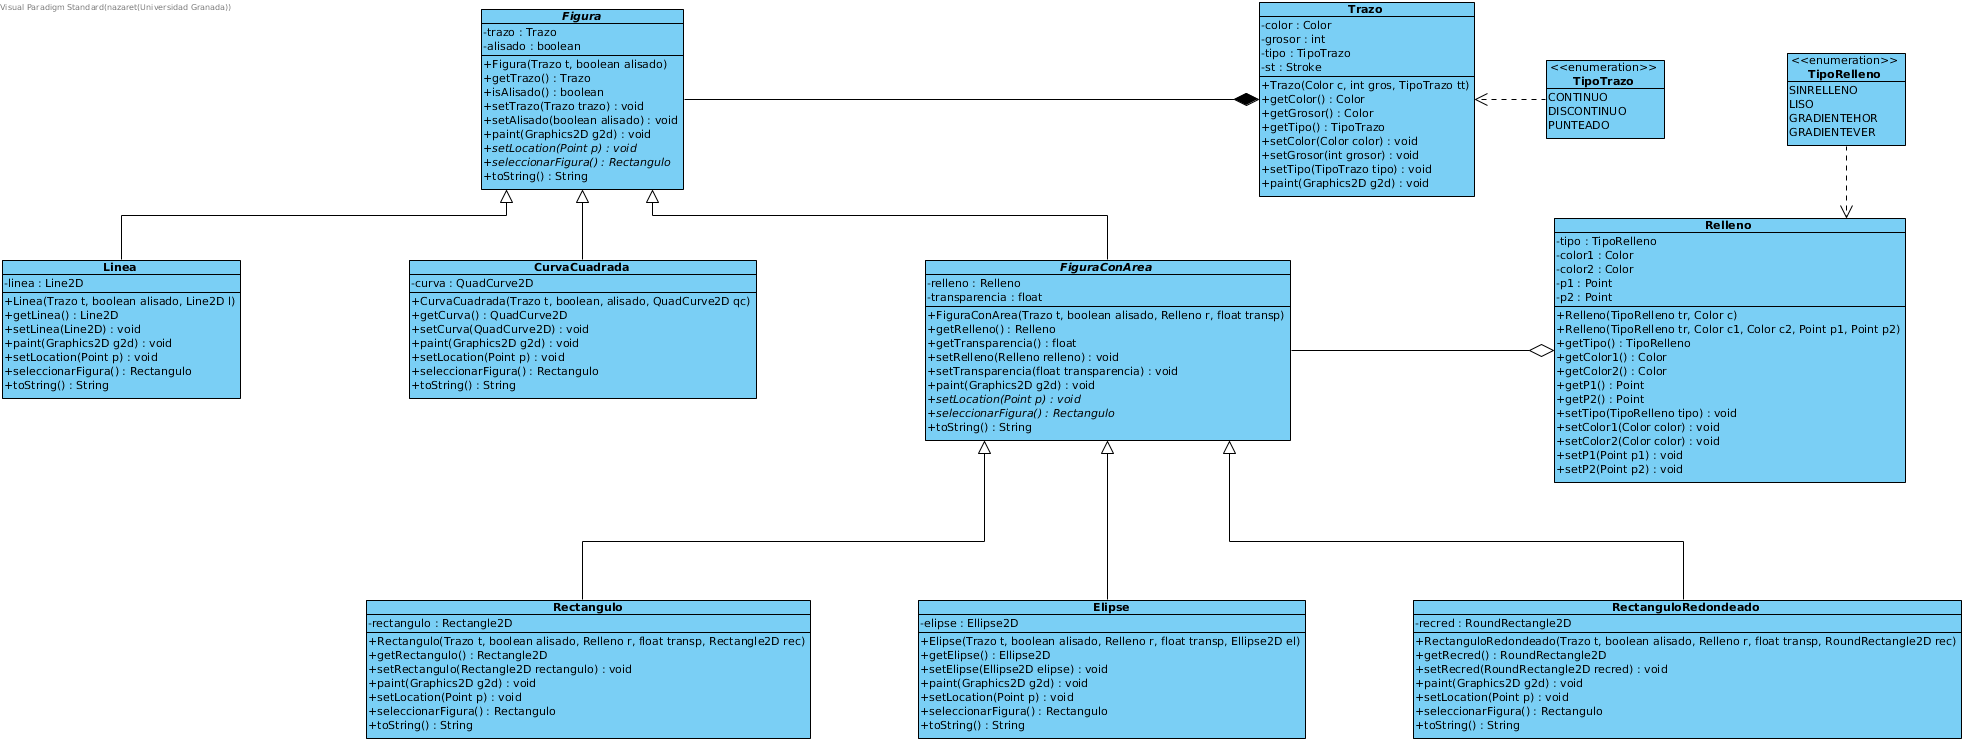
\includegraphics[scale=0.3]{./UML/figuras.png}
\end{figure}

Al igual que ocurre con el diagrama anterior, será incluido con el nombre de \textsc{Figuras.png} para que pueda verse con más fácilidad y que se lean bien los atributos y métodos de cada clase. Además, se incluye el archivo \textsc{General.png} que contiene la unión de ambos diagramas de forma que se pueda ver como funciona la aplicación a grandes rasgos.\\

Como se puede observar en la imagen, se ha definido una jerarquía que consta de una clase abstracta \textsc{Figura}, que contiene un objeto de tipo \textsc{Trazo} con el que se pintarán las figuras.\\

Tanto la línea como la curva implementan directamente de esta clase, ya que no necesitan atributos extra; ni una línea ni una curva tienen relleno, y por tanto, tampoco pueden ser transparentes ya que entonces desaparecerían. Por ese motivo, en mi jerarquía, ni una línea ni una curva pueden tener algún grado de transparencia distinto de 1.0, es decir, opaco.\\

Por otro lado, tenemos la clase \textsc{FiguraConArea} que de nuevo es abstracta, y que hereda directamente de \textsc{Figura}. Esta clase está pensada para figuras que tienen superficie o área y que por tanto, pueden tener un relleno y una transparencia. Por ello esta clase tiene un objeto de tipo \textsc{Relleno}, que contiene todas las características que puede tener, como el color y el tipo de degradado.\\

Por último, nos encontramos con las clases que representan las figuras del rectángulo, la elipse y el rectángulo con las esquinas redondeadas. Estas figuras tienen área por lo que heredan de \textsc{FiguraConArea}.

\subsection{Funcionamiento del sistema}
Los requisitos anteriores se van a ir mostrando ahora paso a paso para demostrar el funcionamiento esperado:

\begin{itemize}
	\item Creación de un nuevo lienzo. El usuario elige las medidas que desea para el lienzo.
	\begin{figure}[H]
	\centering
		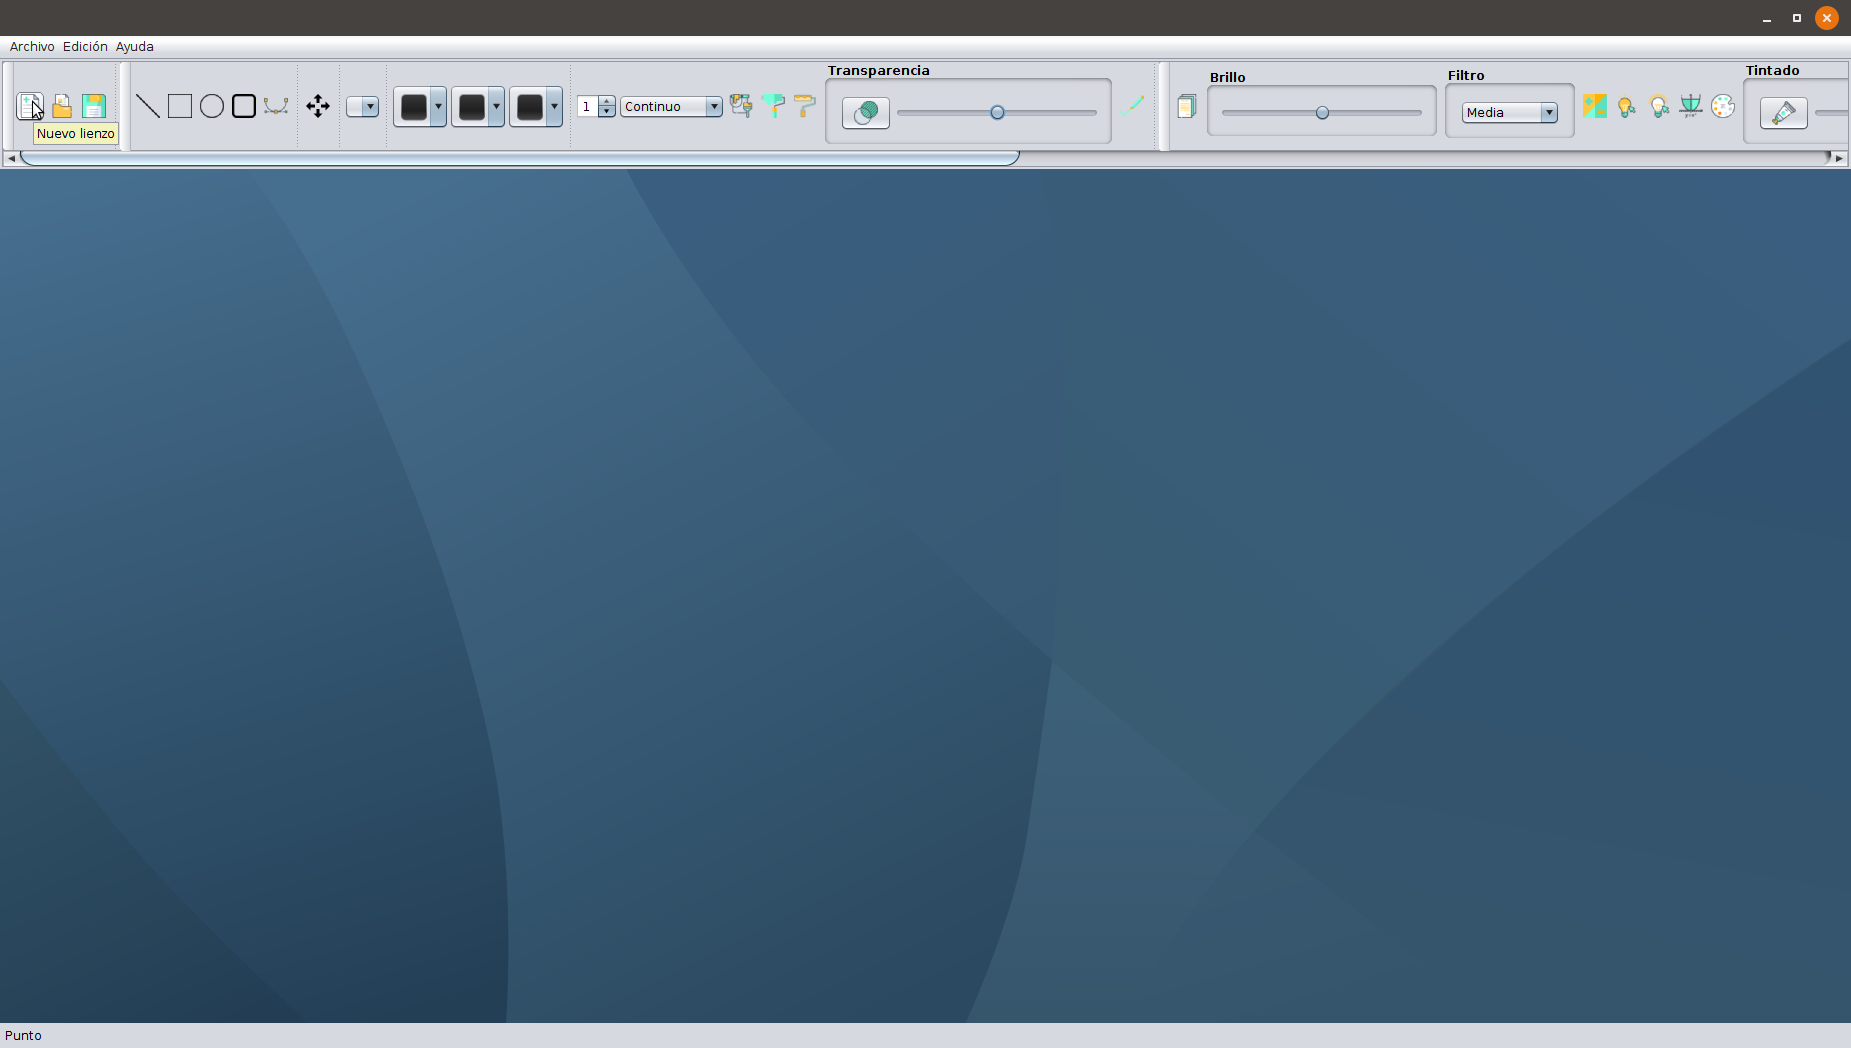
\includegraphics[scale=0.2]{./img/1.png}
	\end{figure}
	\begin{figure}[H]
	\centering
		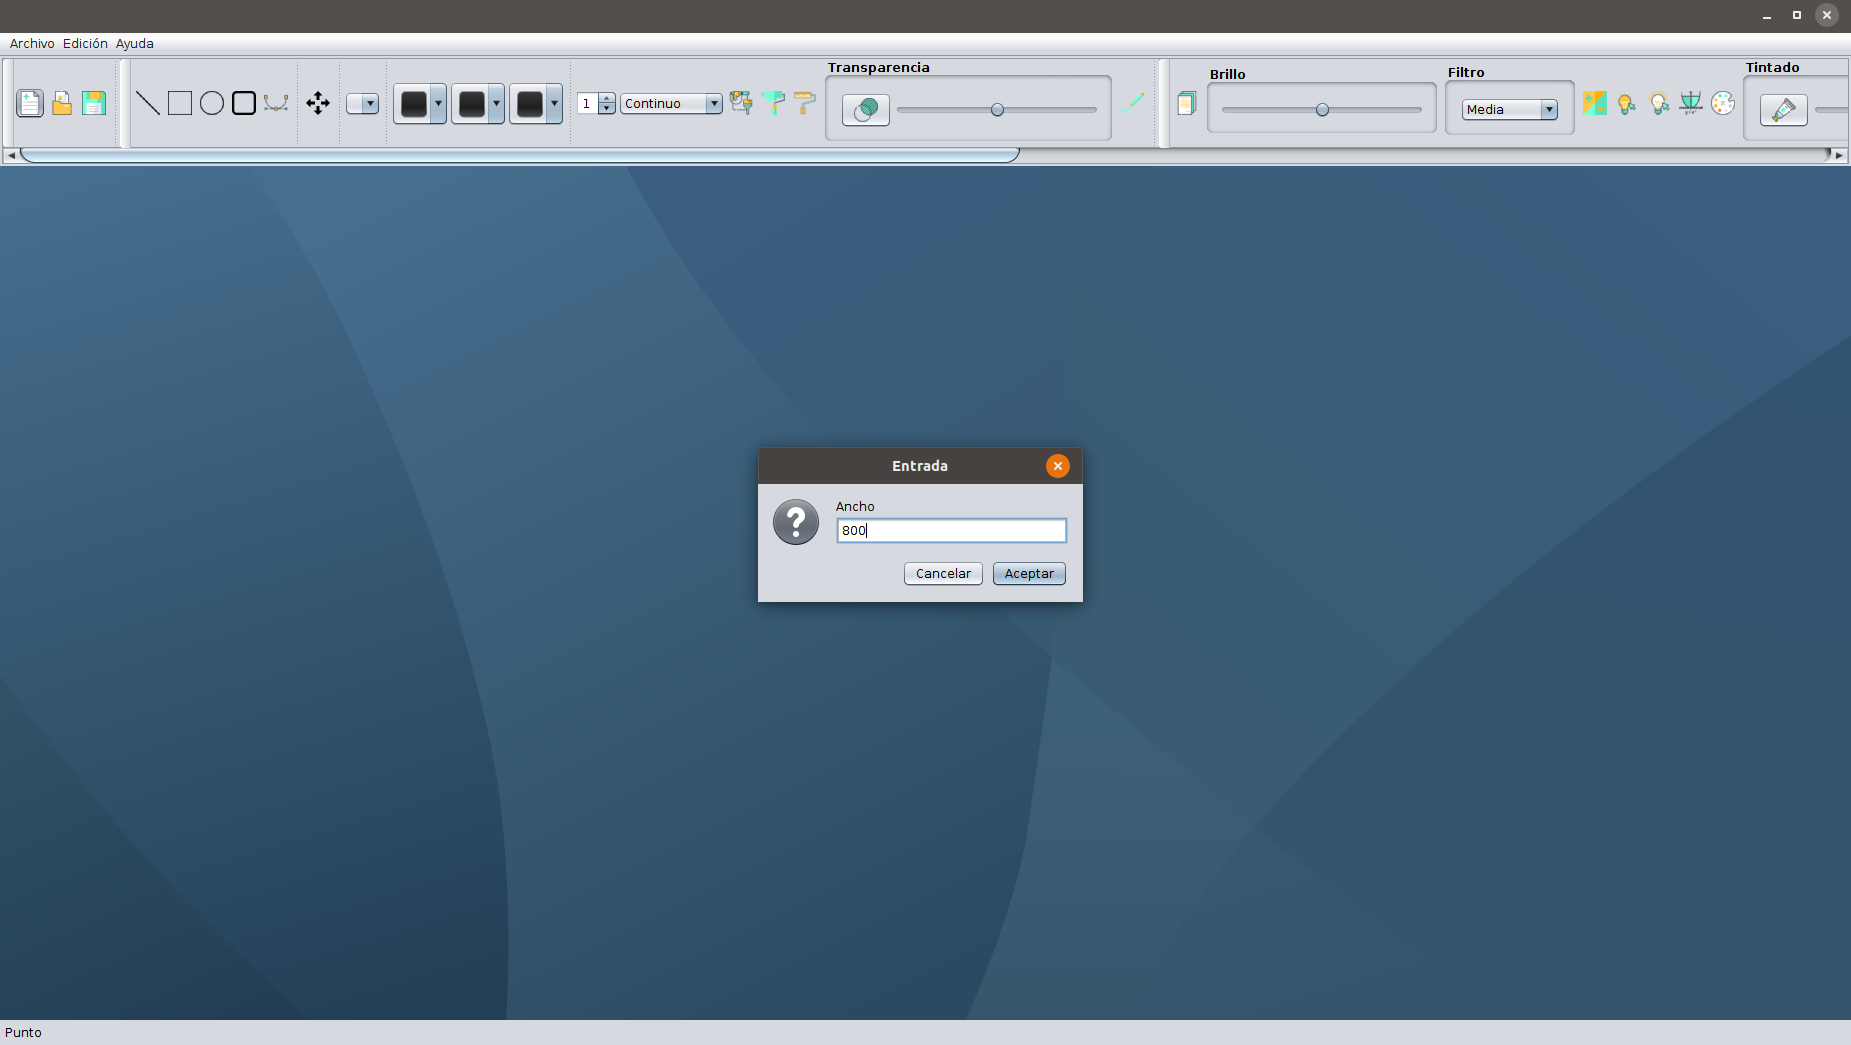
\includegraphics[scale=0.2]{./img/2.png}
	\end{figure}
	\item Se pintan diversas figuras en el lienzo, cada una con sus propiedades. Se muestran todas las formas posibles, el relleno liso, el relleno con gradiente horizontal y el relleno con gradiente vertical.
	\begin{figure}[H]
	\centering
		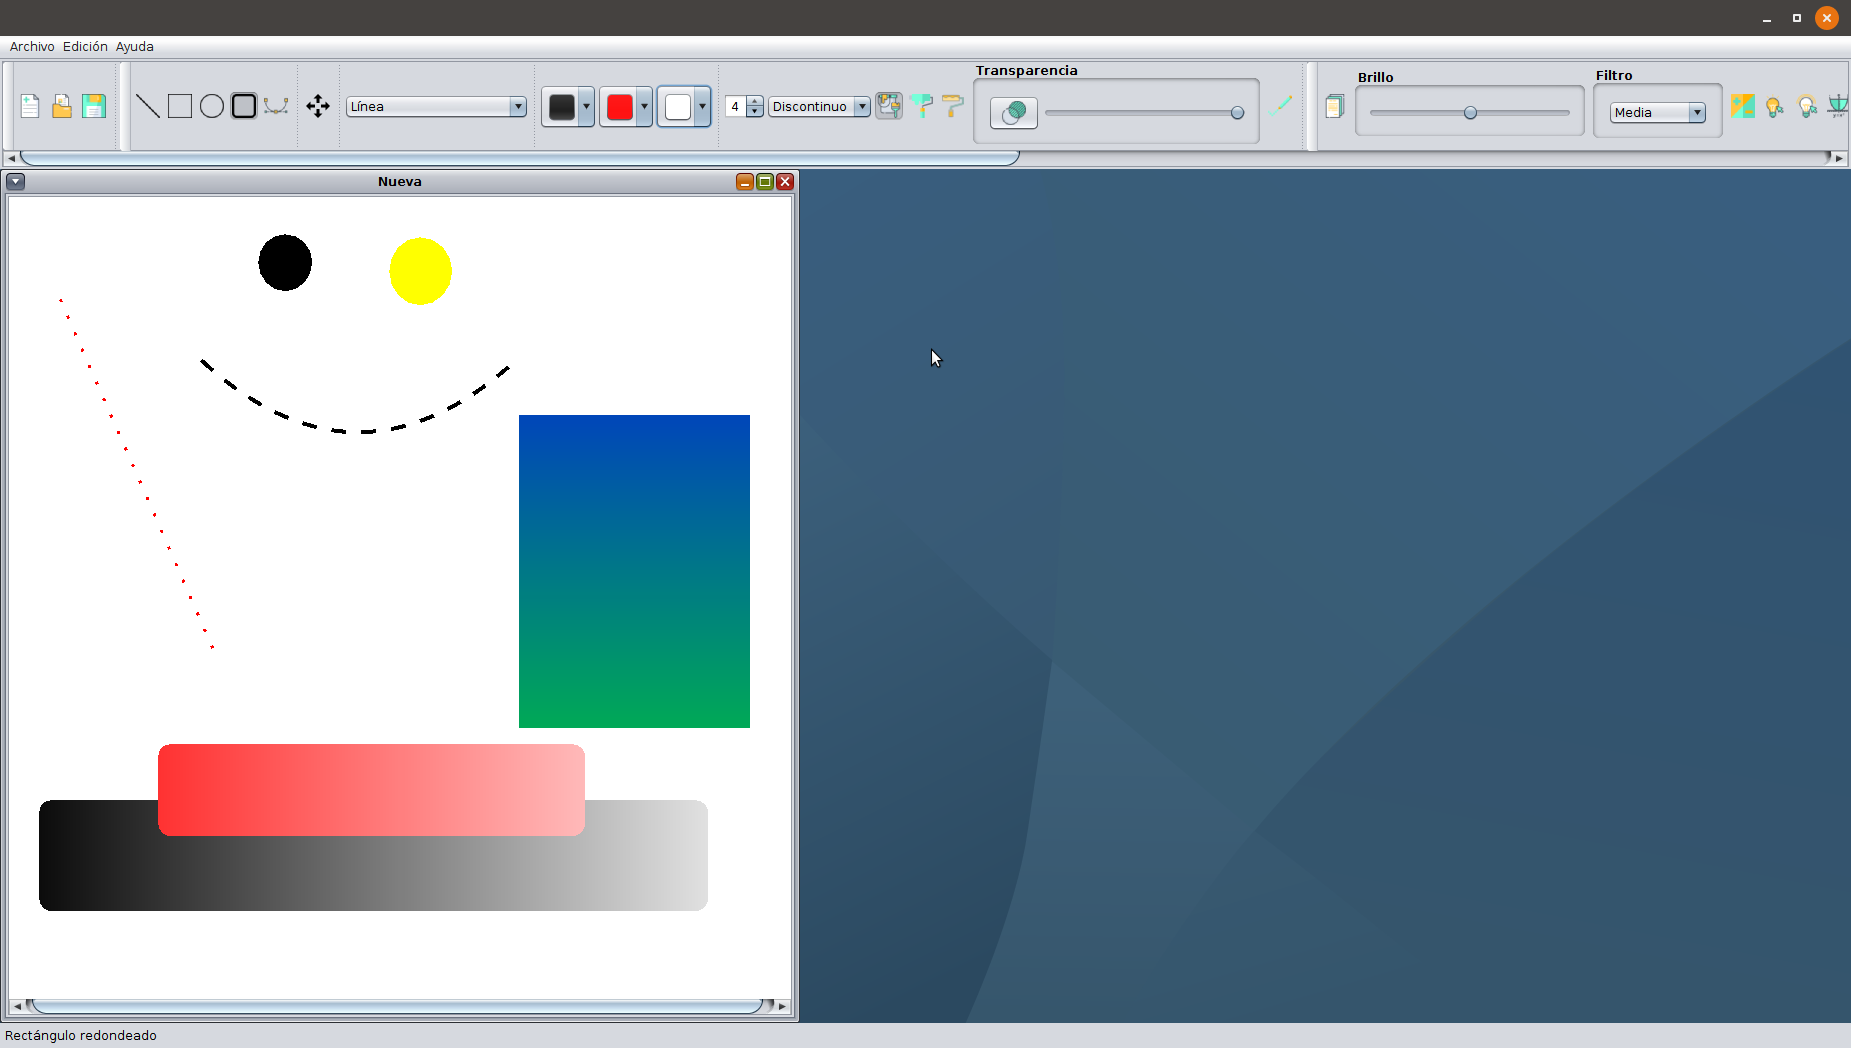
\includegraphics[scale=0.2]{./img/3.png}
	\end{figure}
	\item Seleccionamos dos figuras, primero un rectángulo con degradado y después otra figura, la elipse amarilla. Como se puede observar, al seleccionarlas a través de la lista desplegable, todos los botones y desplegables (excepto el botón de herramienta o aquellos elementos que no tengan valor para la figura seleccionada, como son en este caso, por ejemplo, el segundo color del relleno en la elipse, o el grosor y tipo de trazo) se actualizan en la barra de herramientas, tomando los valores de la figura que hemos seleccionado. Además, se remarca con un rectángulo rojo discontinuo para que sea más sencillo identificar qué figura es.
	\begin{figure}[H]
	\centering
		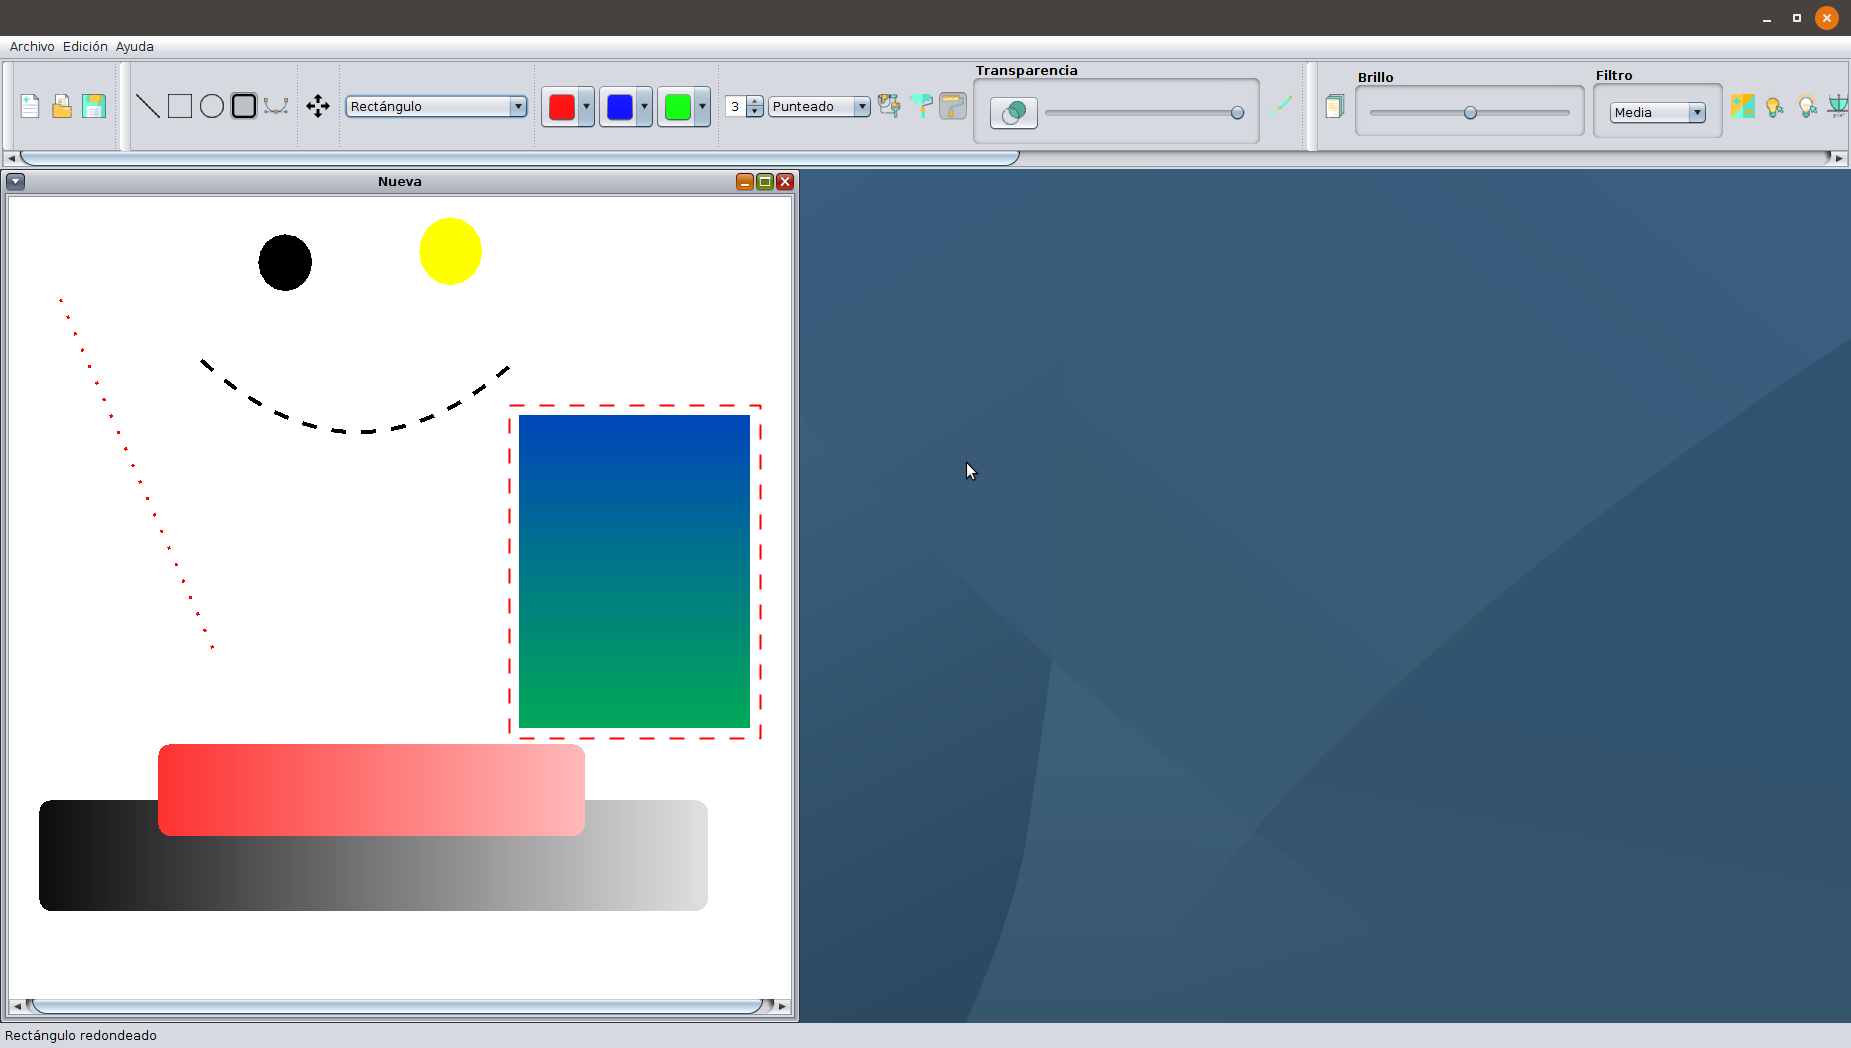
\includegraphics[scale=0.2]{./img/10.png}
	\end{figure}
	\begin{figure}[H]
	\centering
		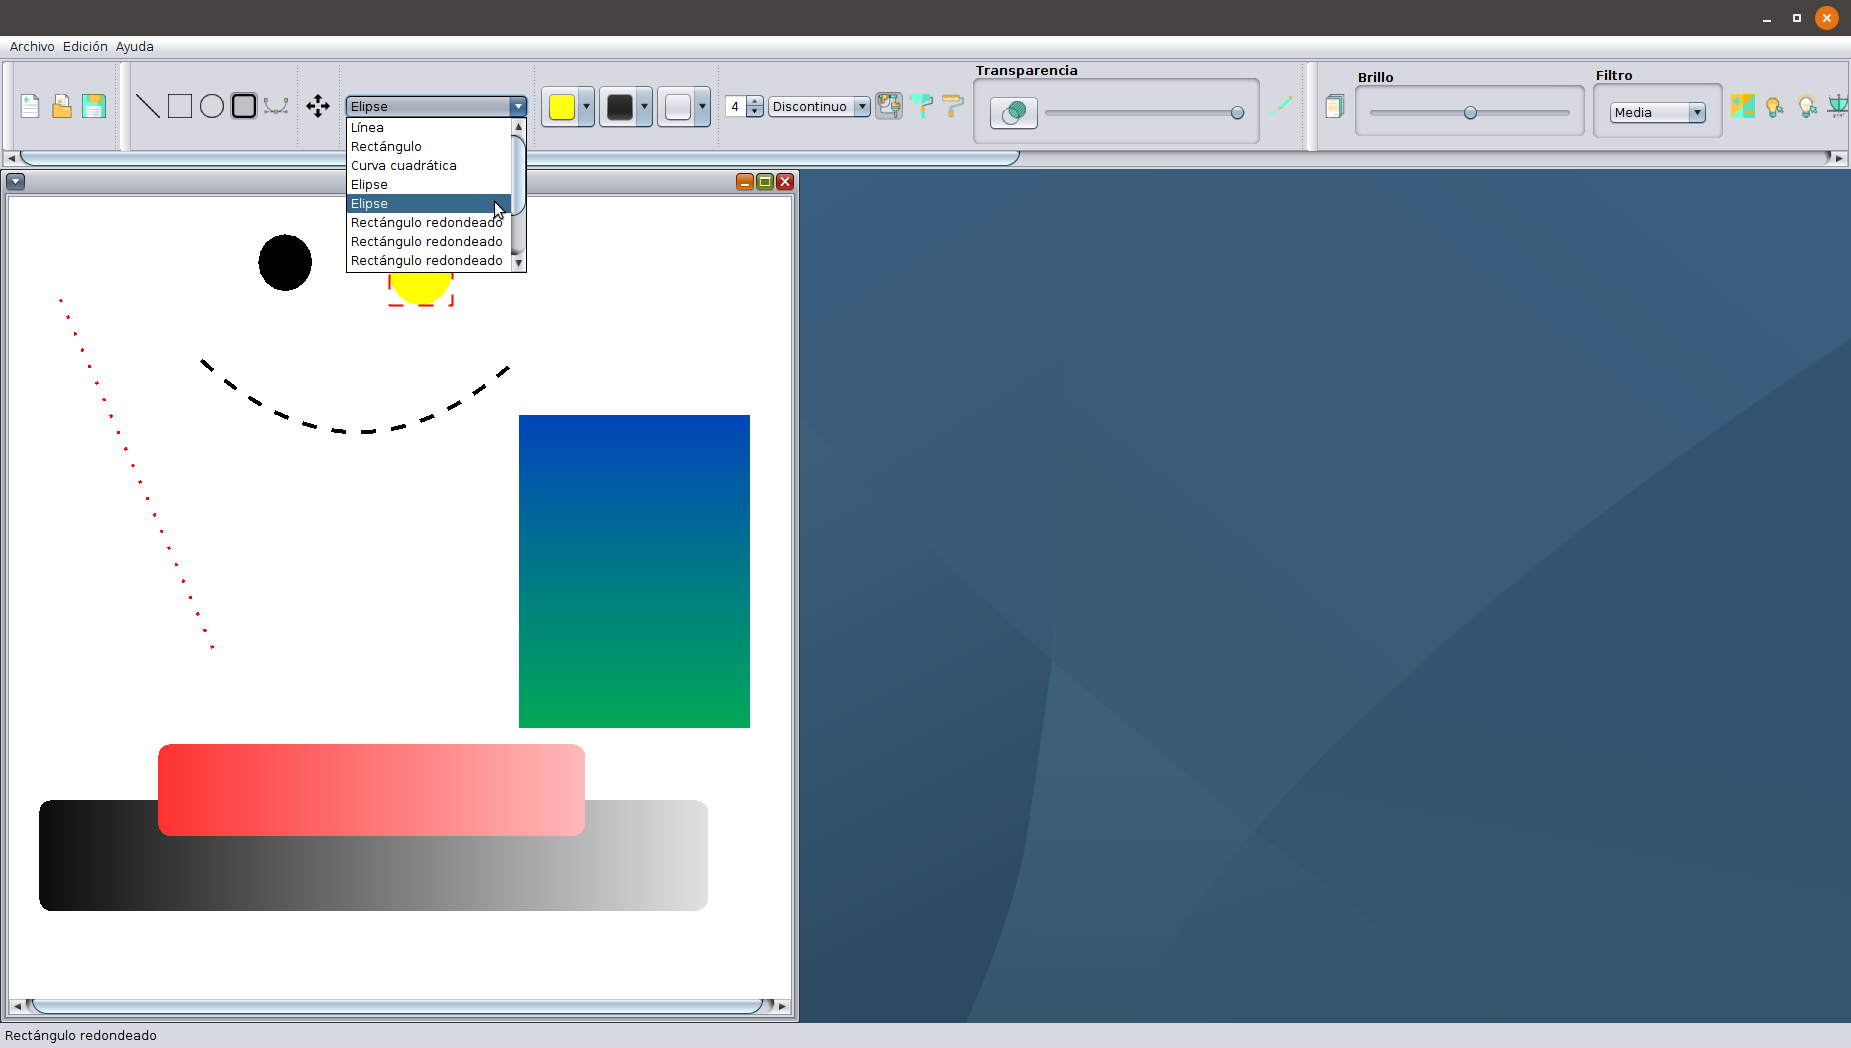
\includegraphics[scale=0.2]{./img/4.png}
	\end{figure}
	\item Ahora vamos a mover la figura seleccionada. Para ello, pulsamos el botón de mover; se abrirán dos diálogos en los que el usuario introducirá el desplazamiento que desea. Éste puede ser negativo en el caso de que se quiera mover hacia arriba o hacia la izquierda y positivo si se quiere mover hacia abajo o hacia la derecha.
	\begin{figure}[H]
	\centering
		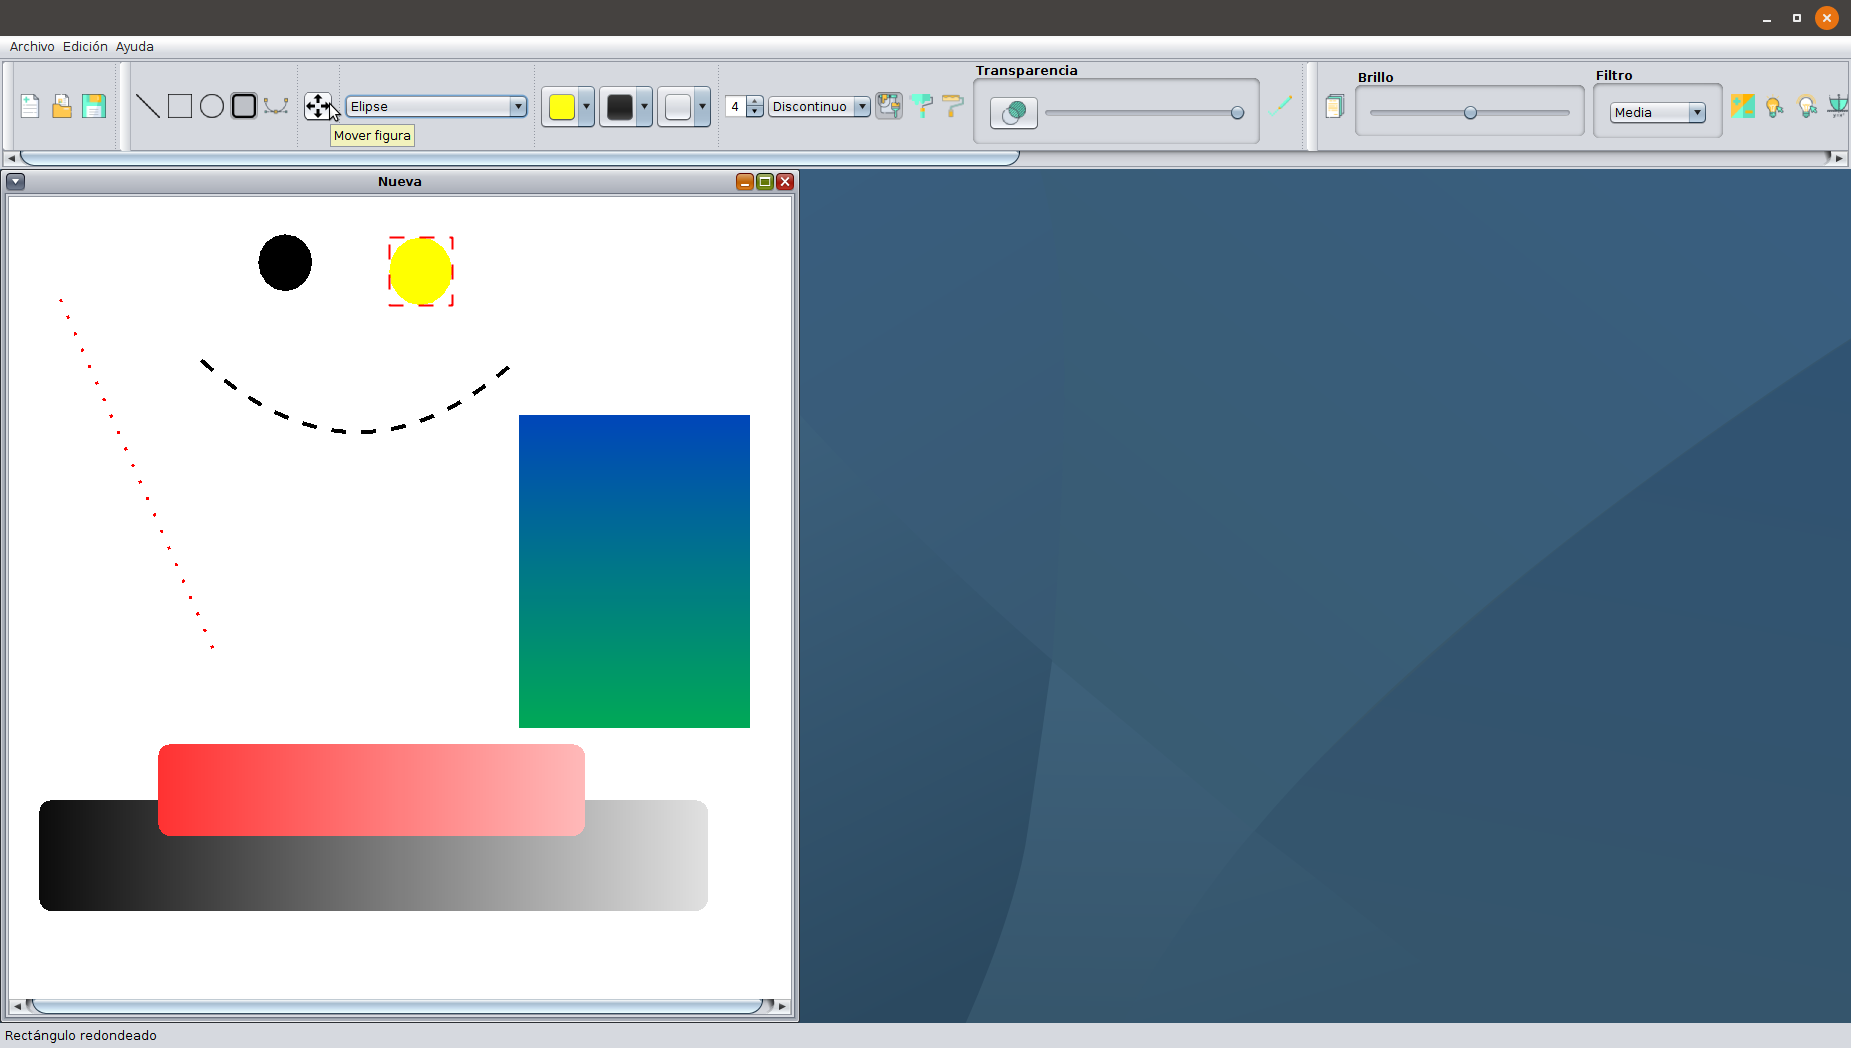
\includegraphics[scale=0.2]{./img/6.png}
	\end{figure}
	\begin{figure}[H]
	\centering
		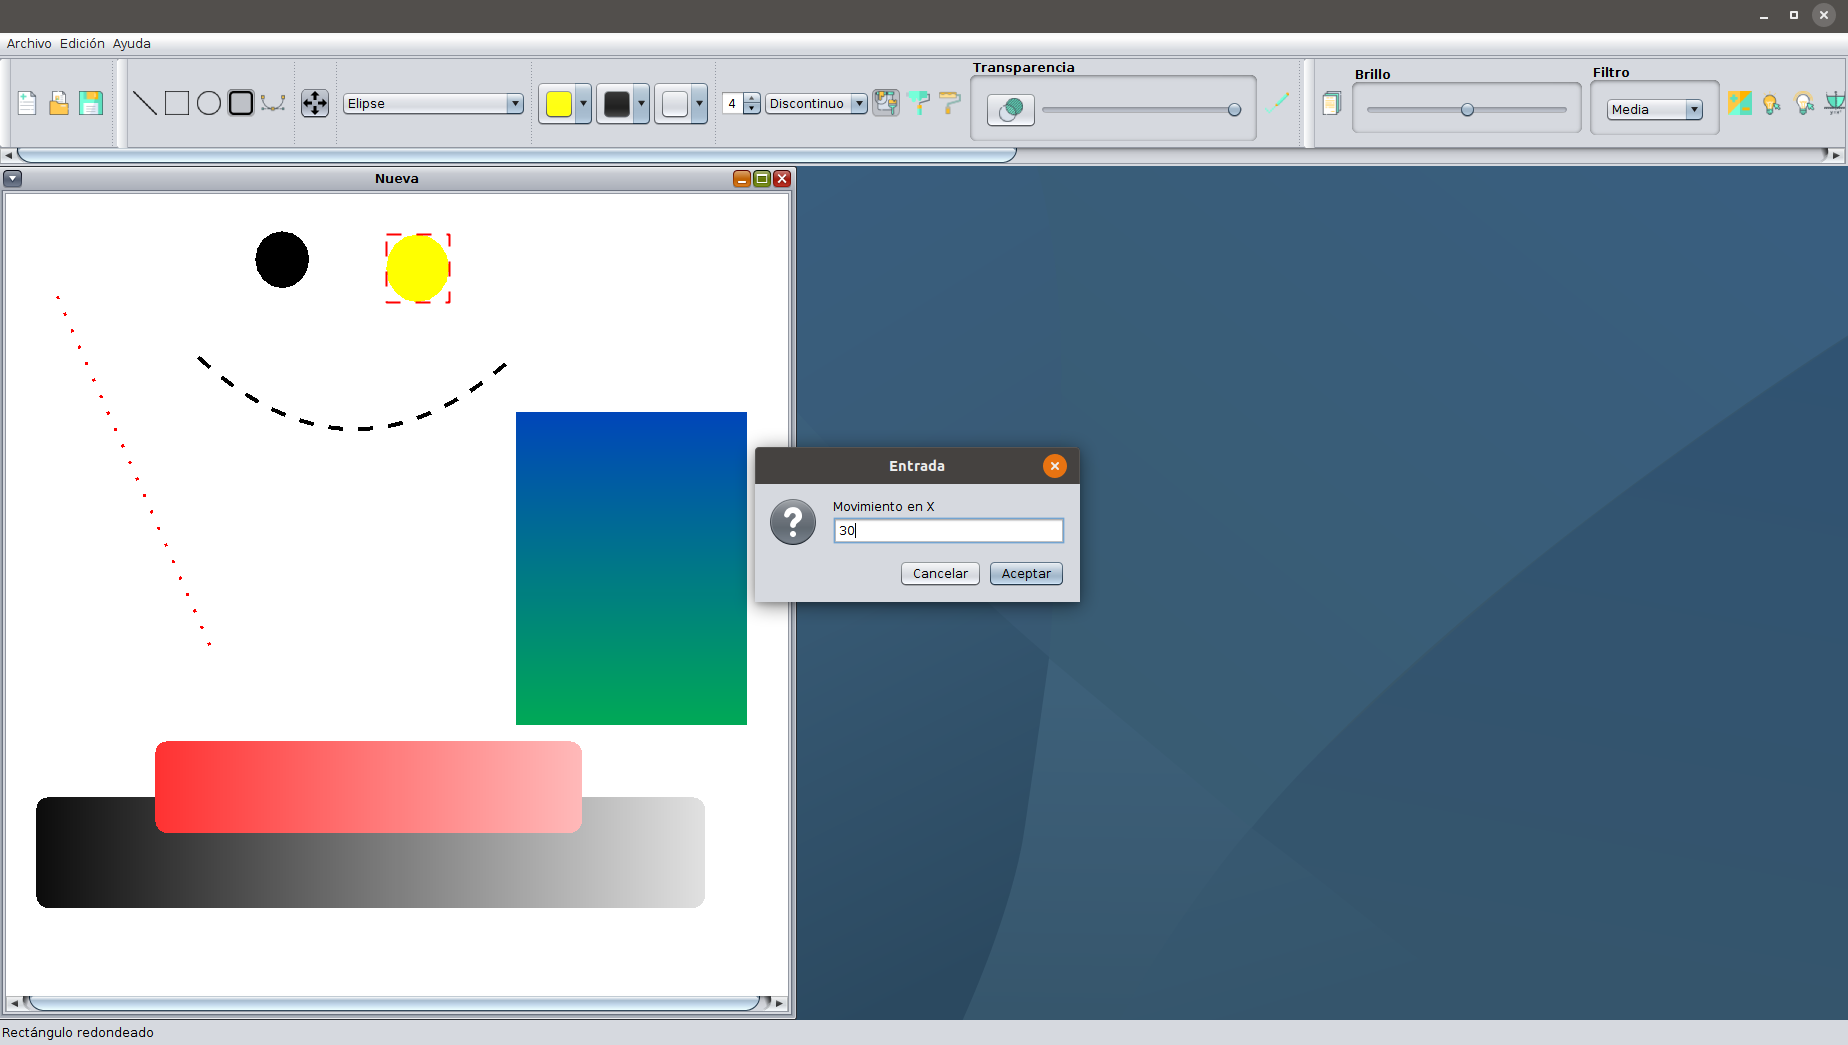
\includegraphics[scale=0.2]{./img/7.png}
	\end{figure}
	\begin{figure}[H]
	\centering
		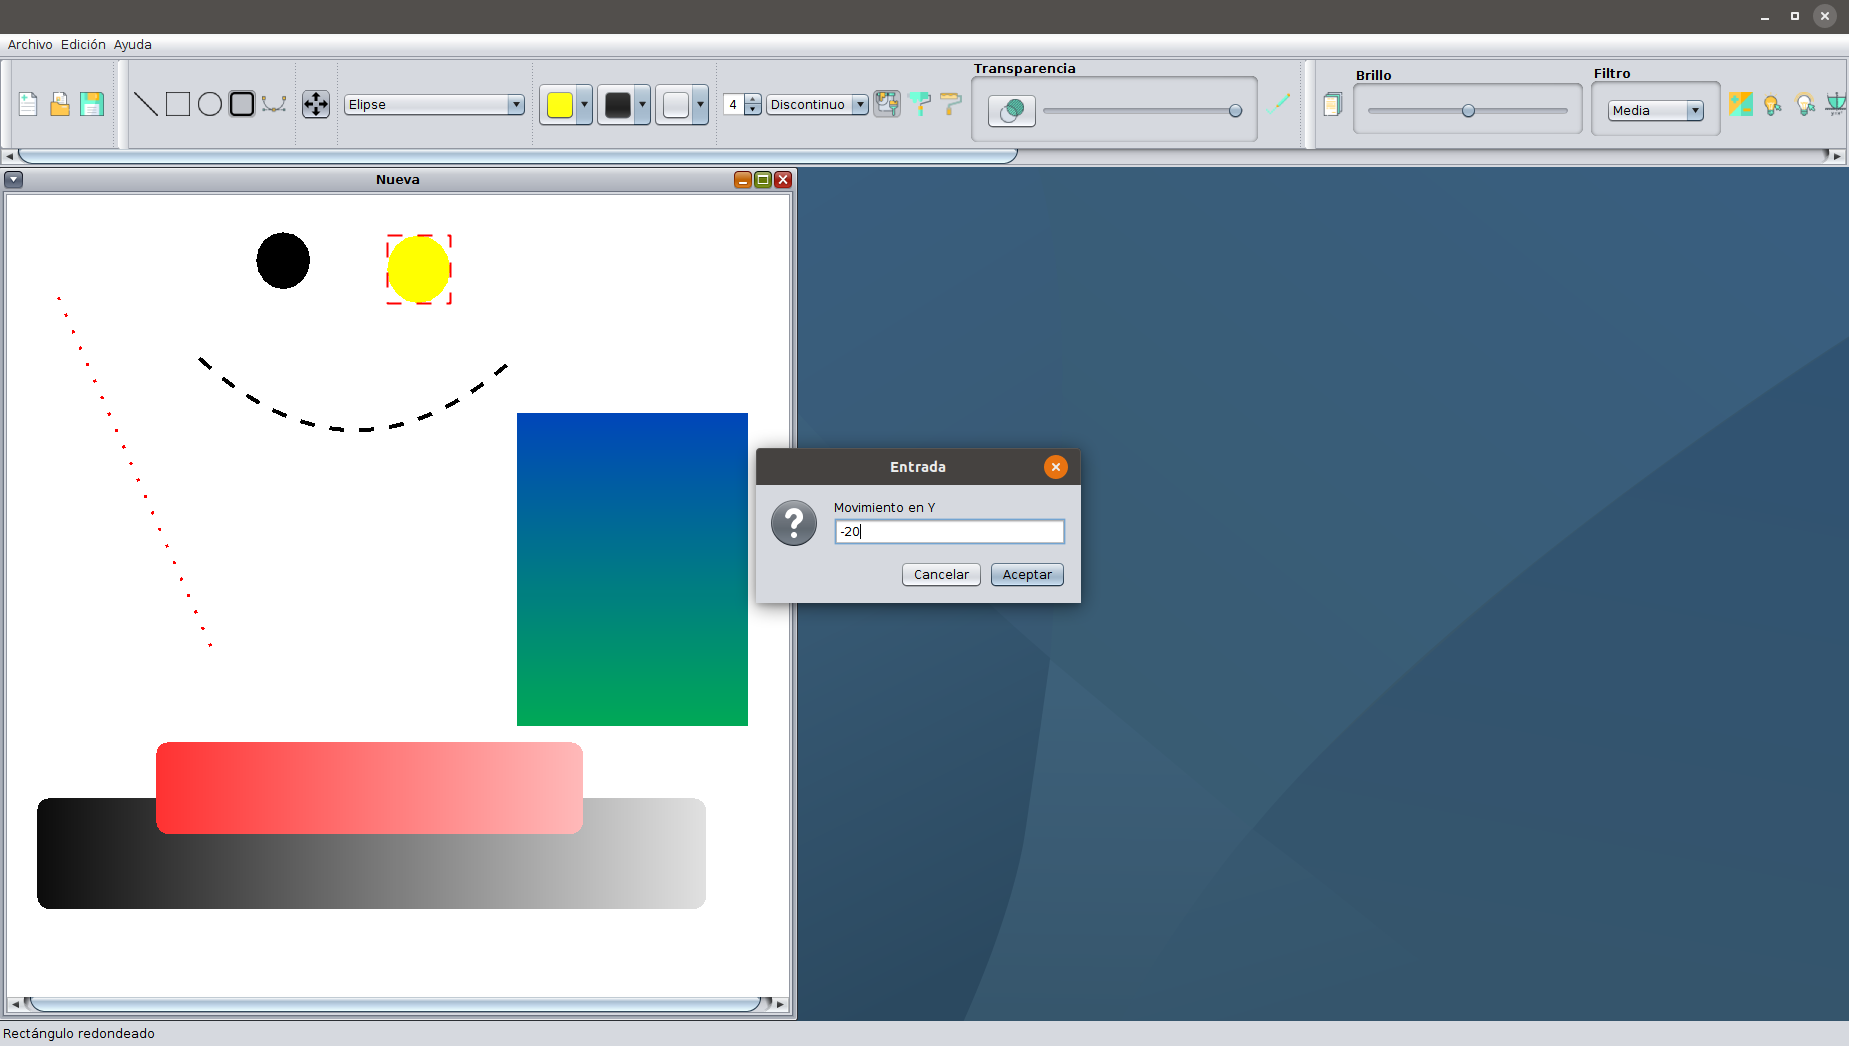
\includegraphics[scale=0.2]{./img/8.png}
	\end{figure}
	\begin{figure}[H]
	\centering
		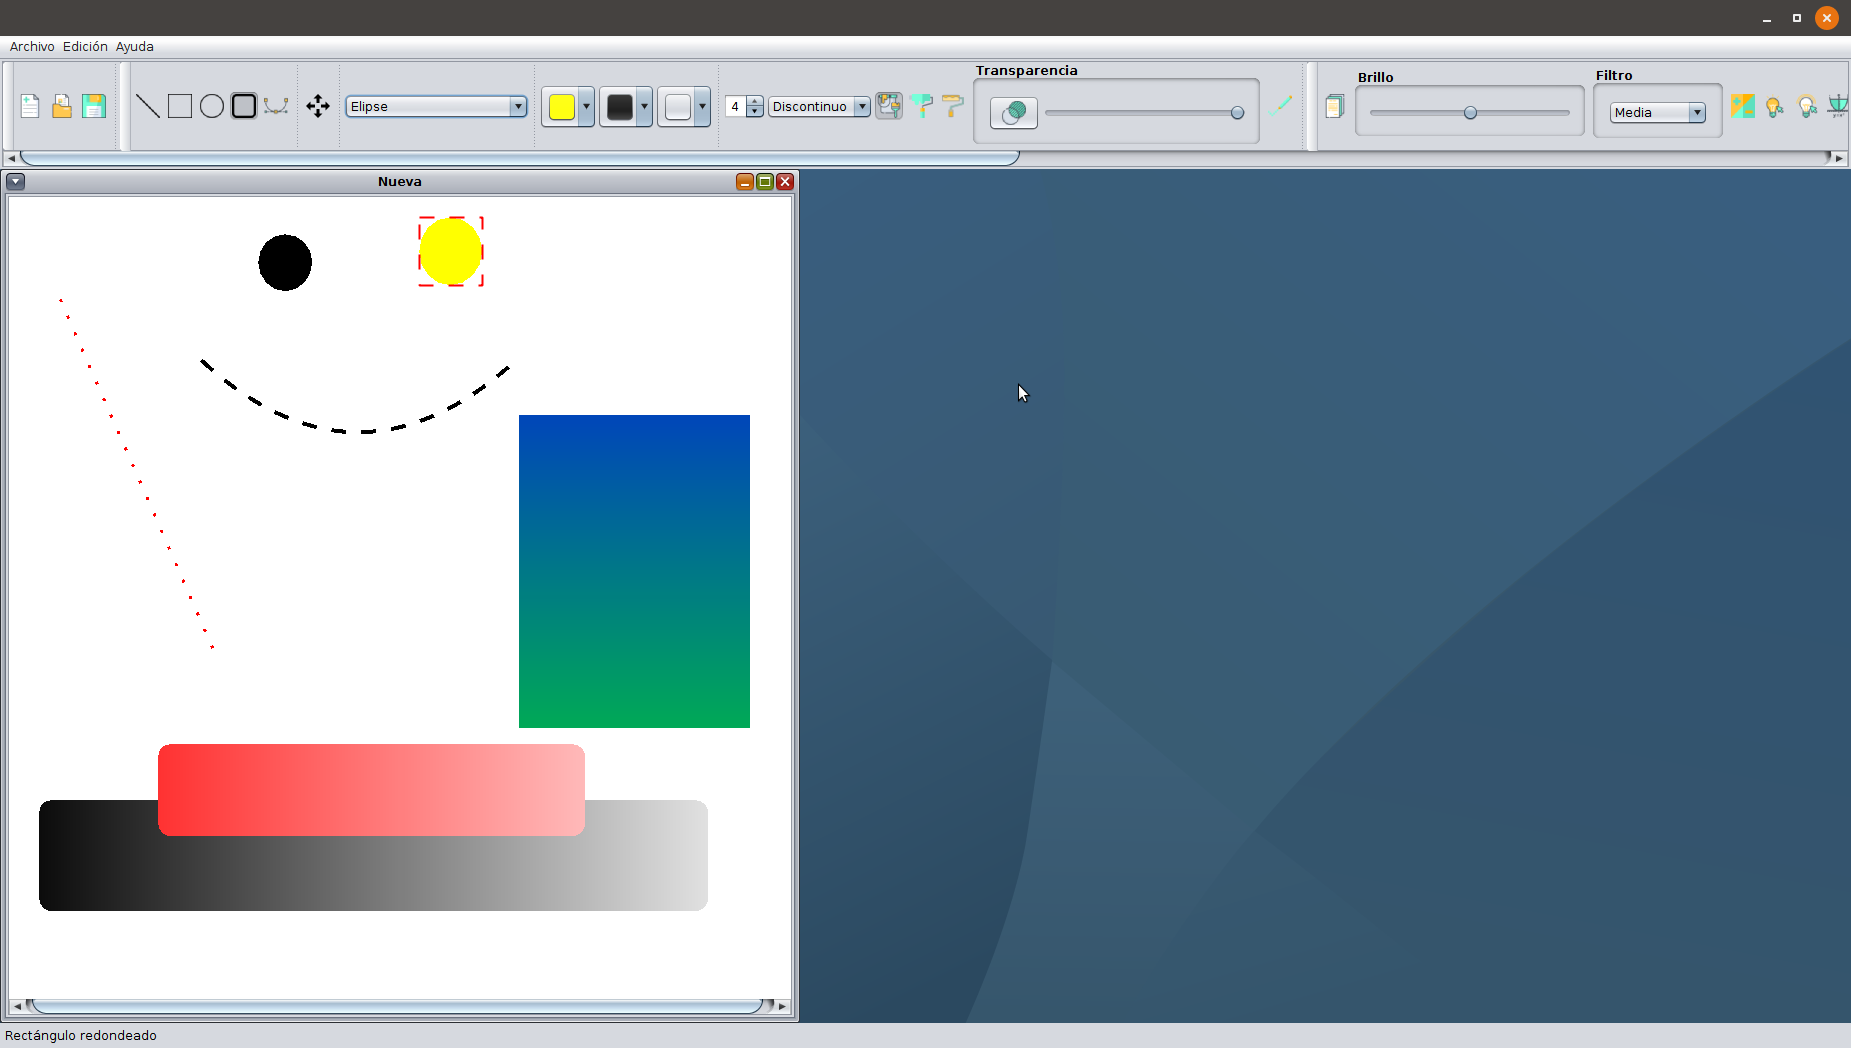
\includegraphics[scale=0.2]{./img/9.png}
	\end{figure}
	\item Ahora modificaremos alguna propiedad de una figura, como por ejemplo la transparencia de la elipse negra. Para ello, en este caso he utilizado el deslizador que varía de totalmente transparente a opaca. No obstante, también está incluido el botón de al lado del deslizador que ofrece la posibilidad de la semitransparencia, es decir, la transparencia con una potencia de 0.5.
	\begin{figure}[H]
	\centering
		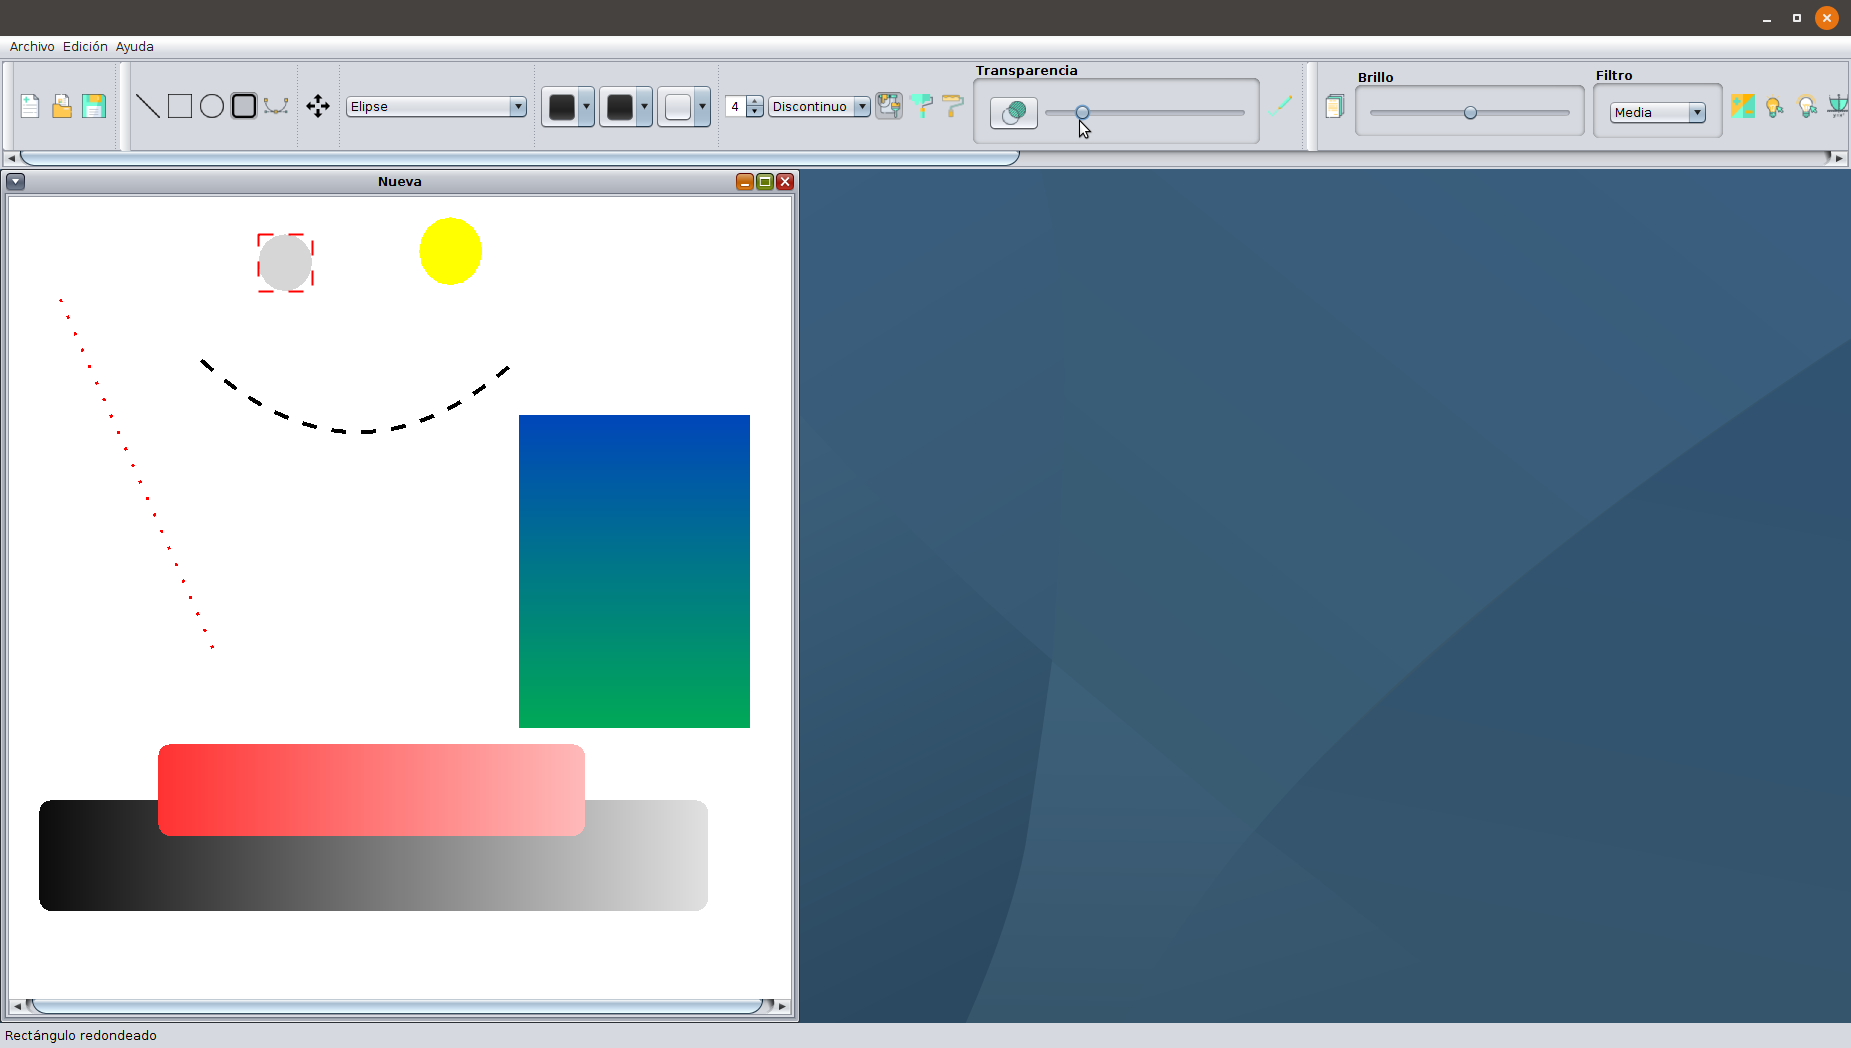
\includegraphics[scale=0.2]{./img/11.png}
	\end{figure}
	\item Como última propiedad que queda por mostrar de las figuras, se muestra el alisado de los bordes, el botón que hay a la derecha del deslizador de transparencia. Para que se vea el efecto, hay dos elipses negras dibujadas, la de la izquierda sin alisado y la de la derecha con alisado. Como se puede observar, el borde de la elipse de la derecha es mucho más suave, sin ``escalones''.
	\begin{figure}[H]
	\centering
		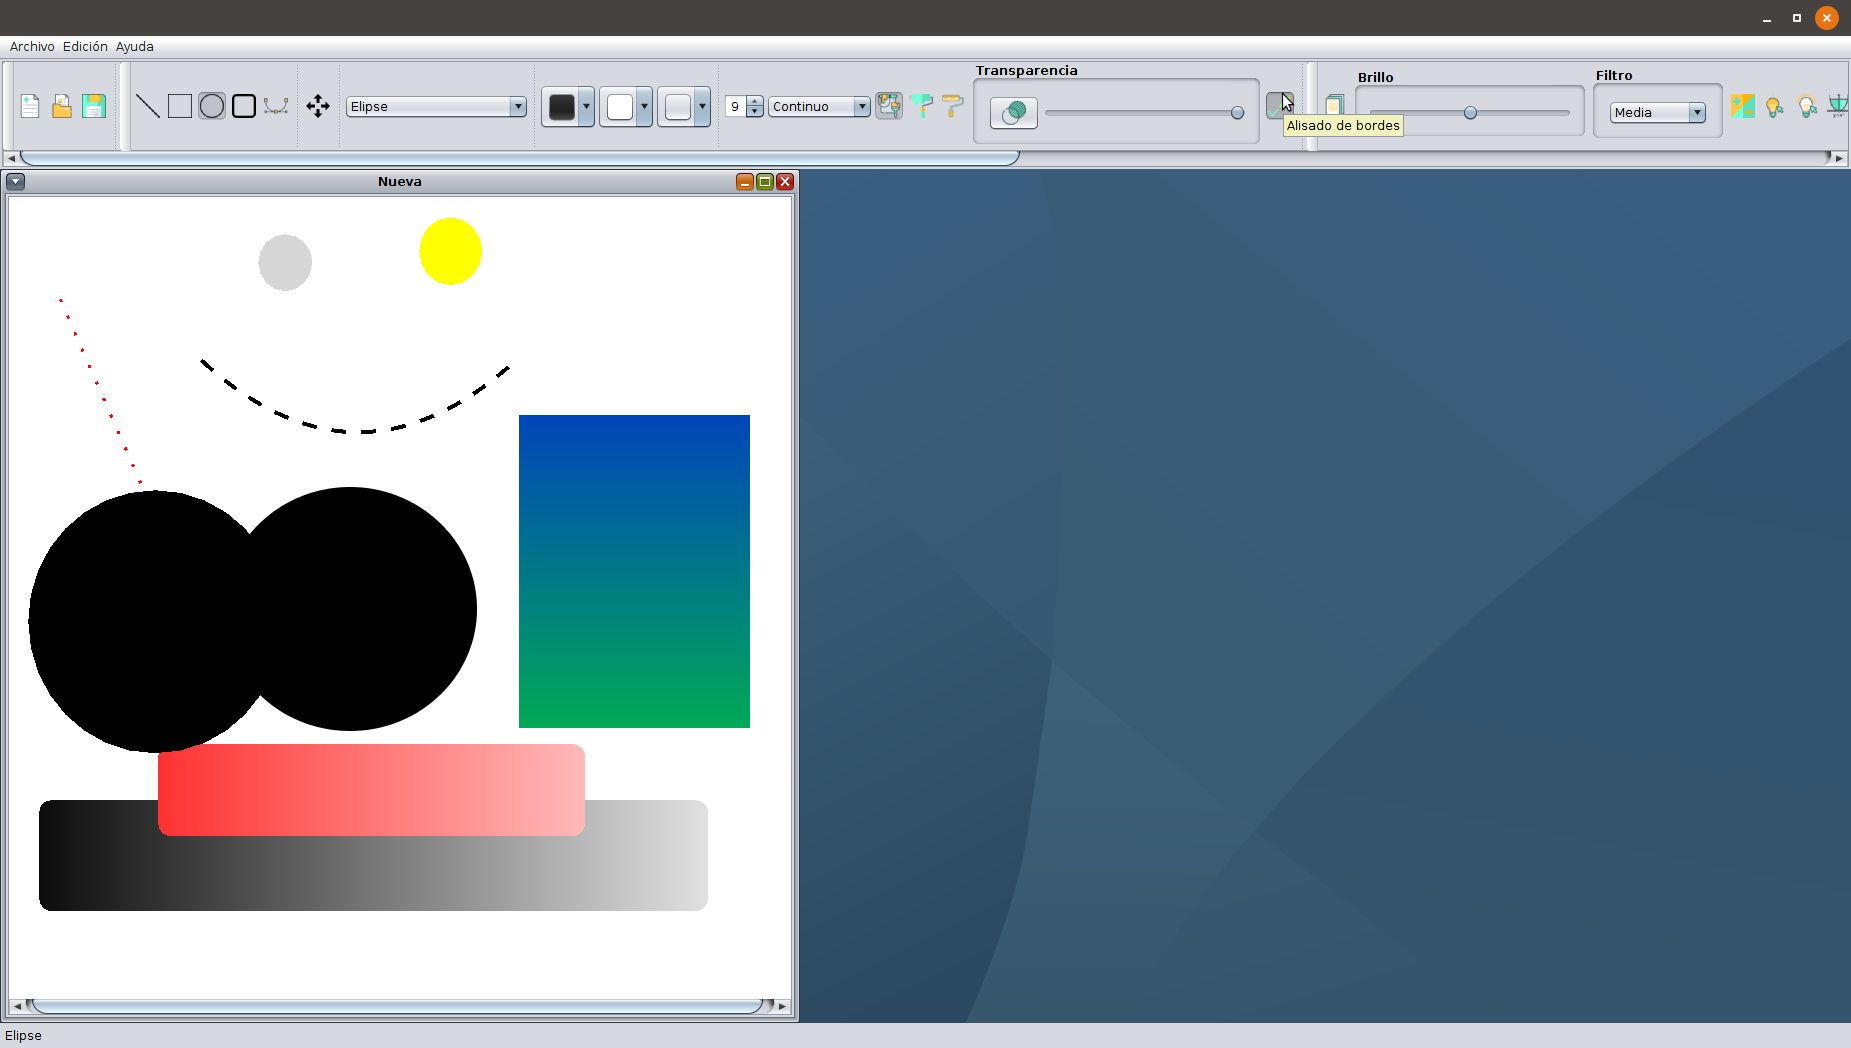
\includegraphics[scale=0.2]{./img/12.png}
	\end{figure}
	\item Ahora, abriremos un nuevo lienzo y observaremos como las propiedades en la barra de herramientas cambian, en este caso a las que tiene un lienzo por defecto.
	\begin{figure}[H]
	\centering
		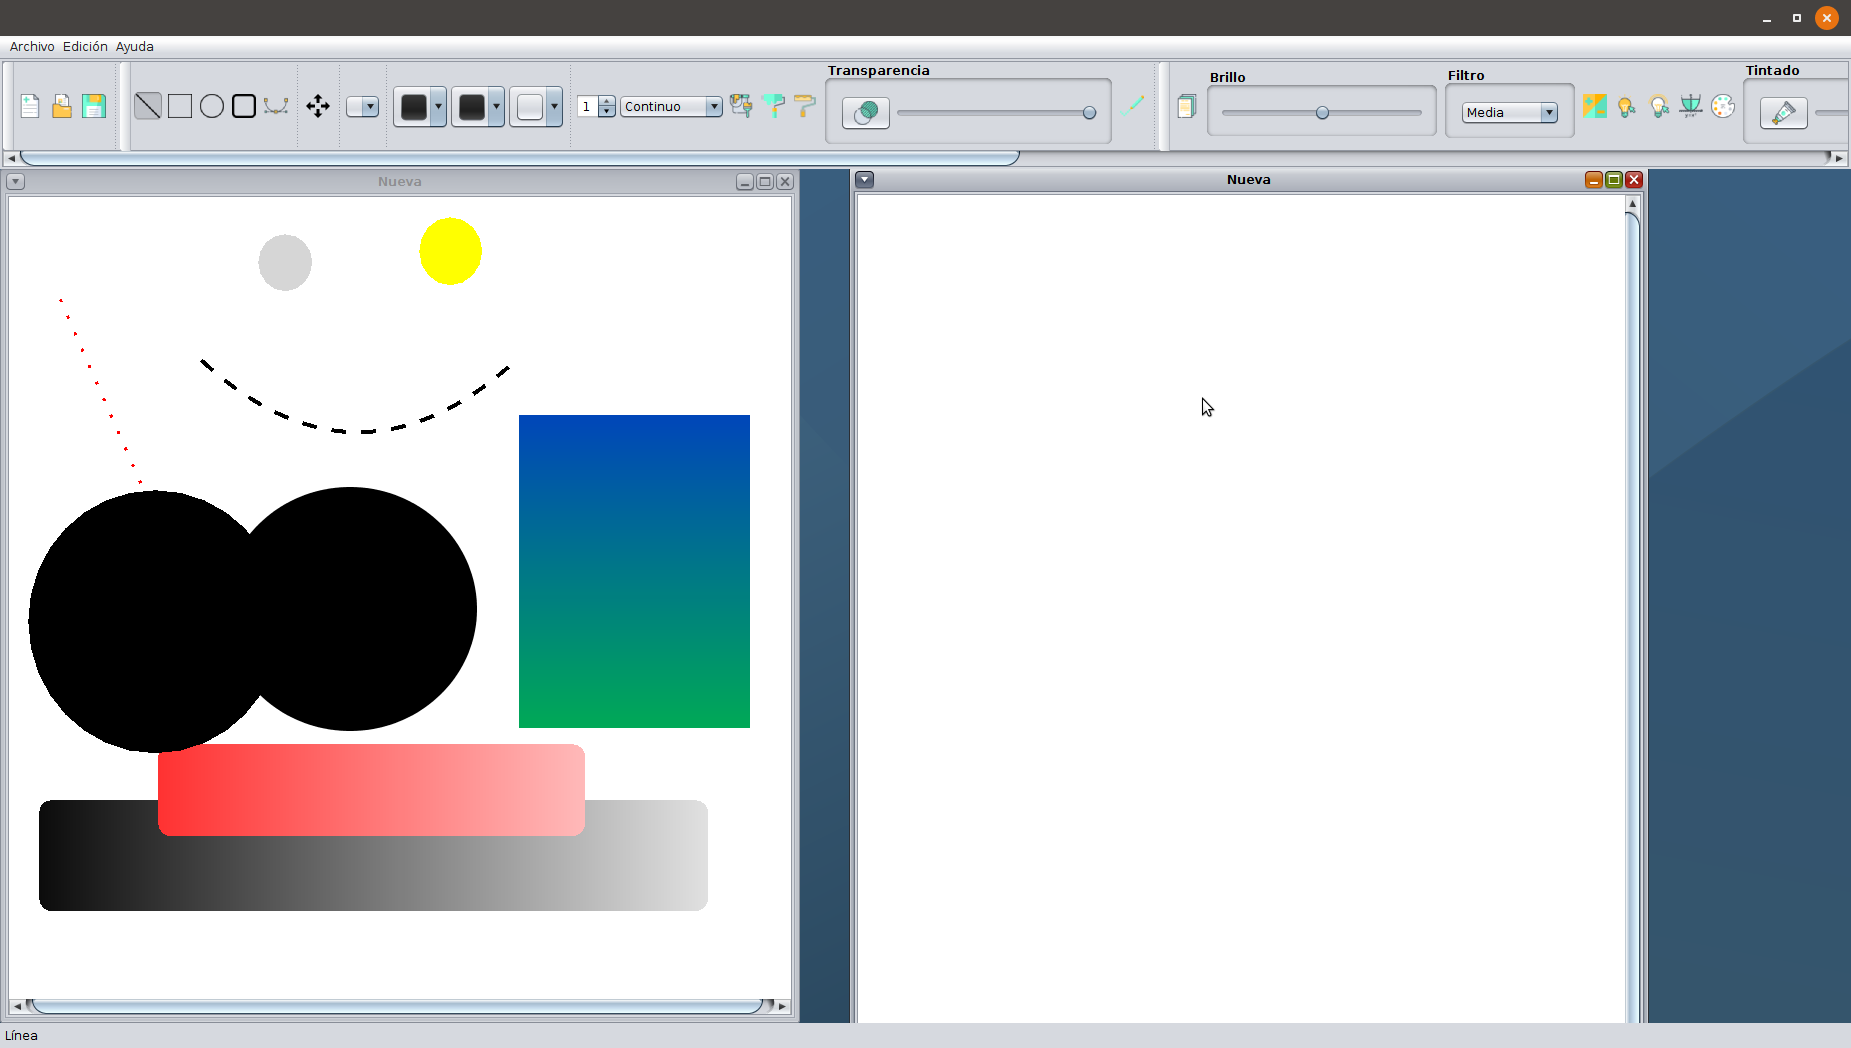
\includegraphics[scale=0.2]{./img/13.png}
	\end{figure}
	\item Por último, se muestra como se puede dibujar sobre lienzos con imágenes y también procesar dichas imágenes. Las figuras que se dibujen se mantendrán solo dentro de la propia imagen, es decir, las figuras no se pintarán sin sobrepasan los límites de la imagen, como se puede observar en la priemera imagen. Además, se puede procesar la fotografía poniendo filtros sobre esta, rotándola... aunque estos efectos no se verán reflejados sobre las figuras.
	\begin{figure}[H]
	\centering
		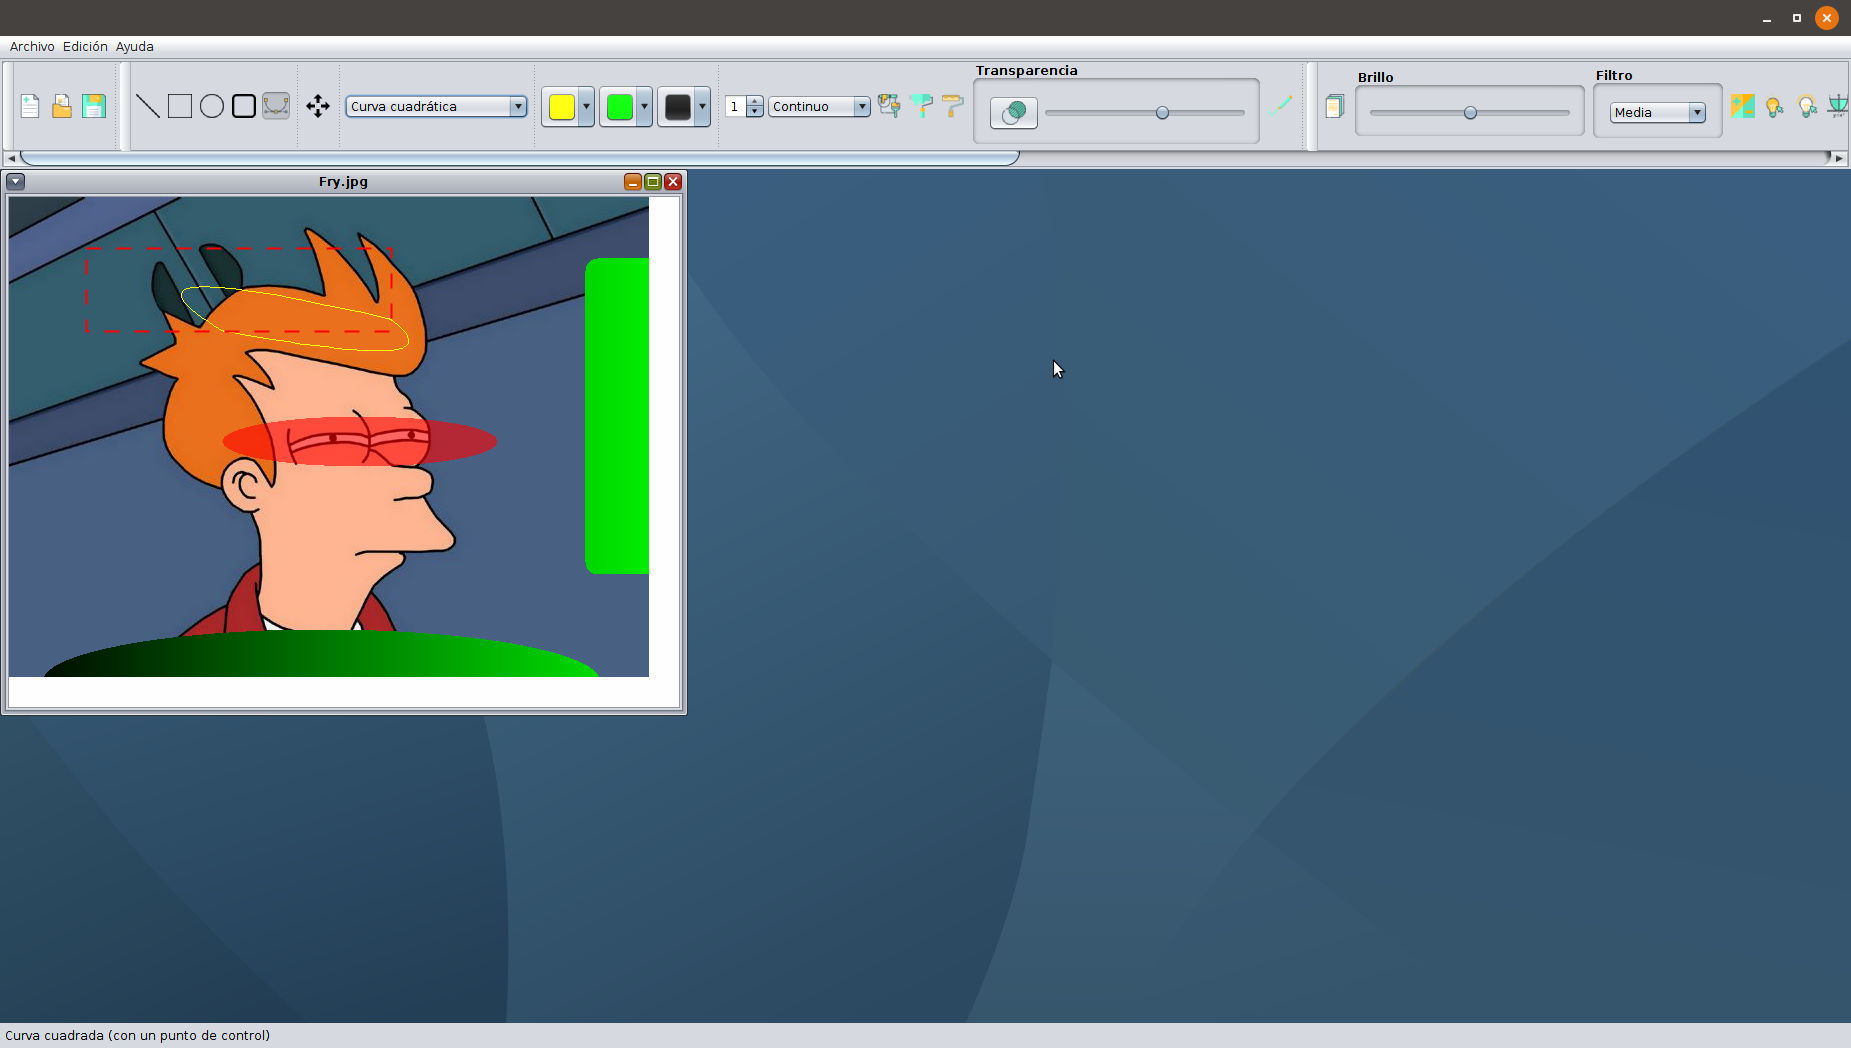
\includegraphics[scale=0.2]{./img/14.png}
	\end{figure}
	\begin{figure}[H]
	\centering
		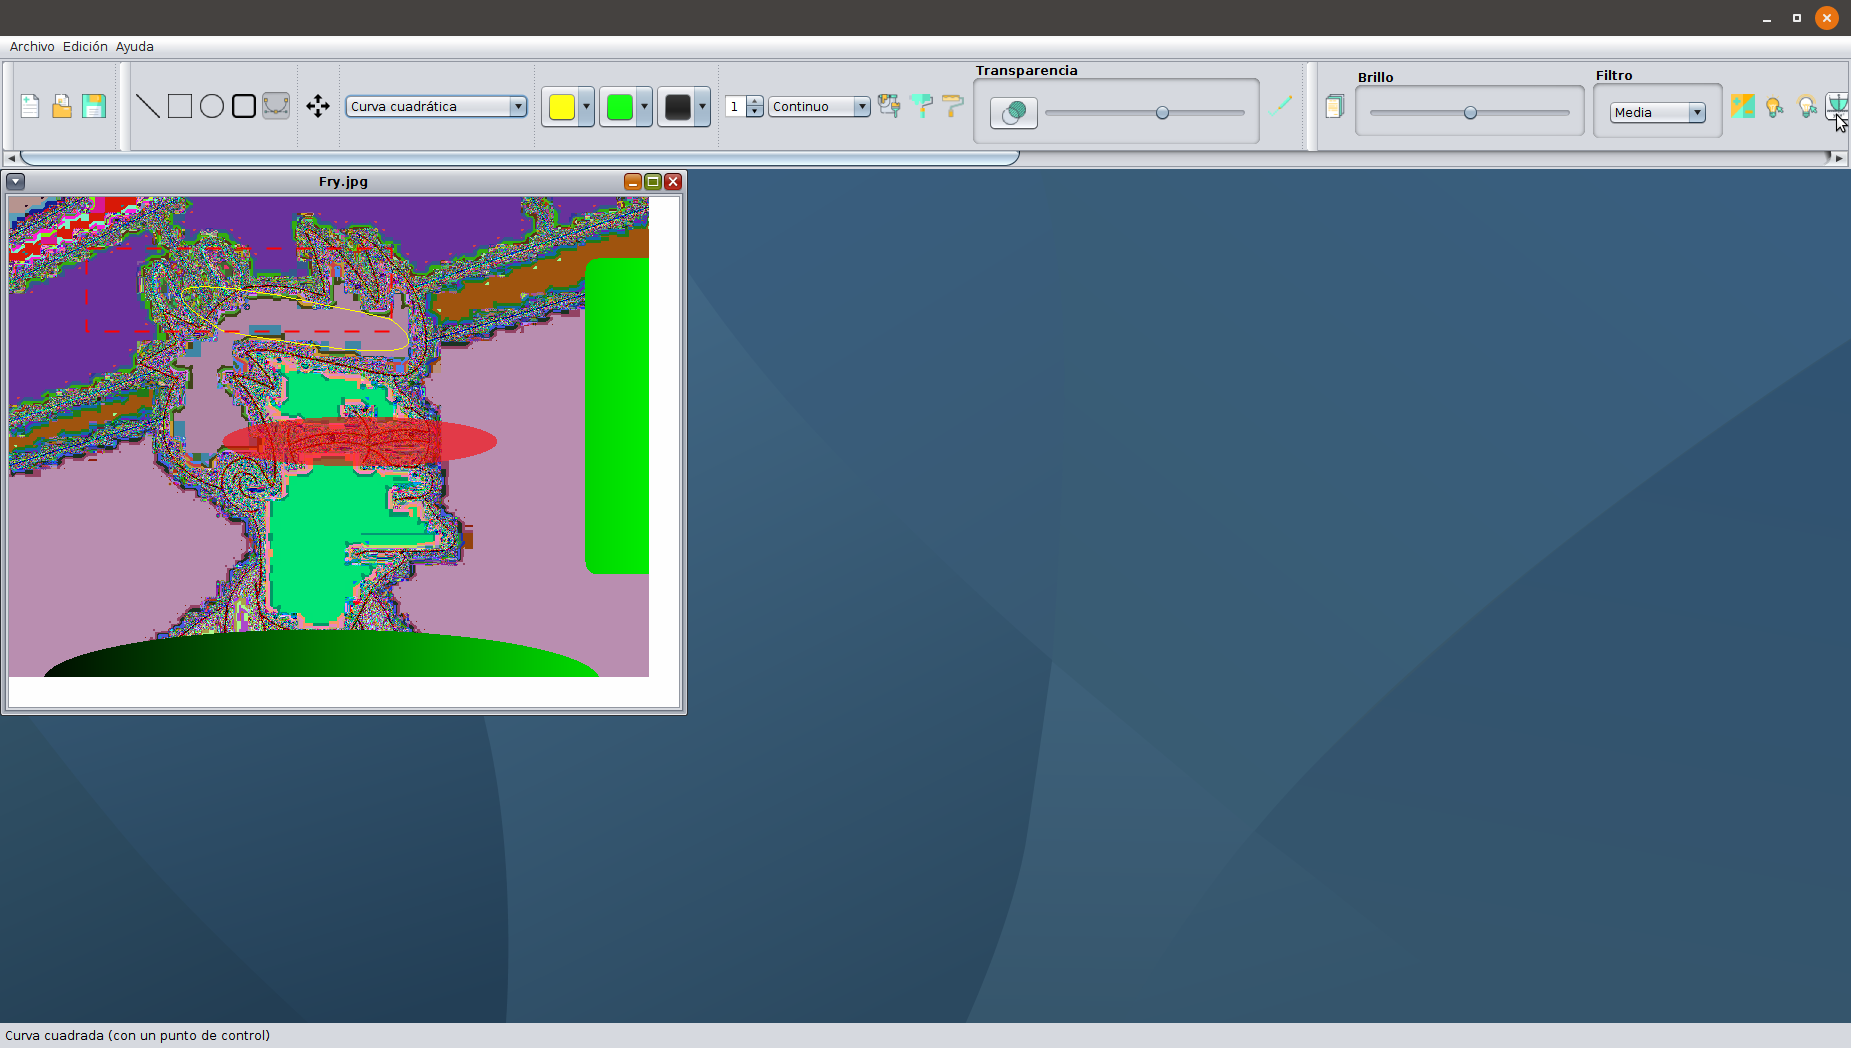
\includegraphics[scale=0.2]{./img/15.png}
	\end{figure}
\end{itemize}

\newpage

\section{Imagen}

\subsection{Análisis de requisitos}
En la parte de procesamiento de imágenes, los requisitos funcionales que se le piden al sistema son:

\begin{itemize}
	\item RF1. Duplicado de imágenes.
	\item RF2. Modificación del brillo mediante un deslizador.
	\item RF3. Filtro de emborronamiento.
	\item RF4. Filtro de enfoque.
	\item RF5. Filtro de relieve.
	\item RF6. Contraste.
	\item RF7. Contraste con iluminación.
	\item RF8. Contraste con oscurecimiento.
	\item RF9. Efecto negativo.
	\item RF10. Extracción de bandas de la imagen.
	\item RF11. Conversión a distintos espacios de color (RGB, YCC, GRAY).
	\item RF12. Rotación de la imagen mediante un deslizador.
	\item RF13. Zoom-in.
	\item RF14. Zoom-out.
	\item RF15. Efecto tintado con el color seleccionado.
	\item RF16. Ecualización de la imagen.
	\item RF17. Filtro sepia.
	\item RF18. Umbralización en niveles de gris mediante un deslizador.
	\item RF19. Filtro basado en la función $f(x)=|x^3+|\cos(xw)|+1)|\%255$.
	\item RF20. Filtro termal.
	\item RF21. Filtro rayos-x.
	\item RF22. Suma de imágenes.
	\item RF23. Resta de imágenes.
	\item RF24. Efecto tintado con el color seleccionado mediante un deslizador.
\end{itemize}

\subsection{Explicación de cada requisito}

Para cada requisito mencionado previamente, se pide al sistema que efectúe lo siguiente:

\begin{itemize}
	\item RF1. Se debe crear una copia de la imagen independiente. Una vez creada, su título será el título de la imagen original unido a la palabra ``copia''.
	\item RF2. El deslizador indicará el brillo que se le aplicará a la imagen que se está procesando.
	\item RF3. Se llevará a cabo el emborronamiento de la imagen cuando se seleccione esta opción.
	\item RF4. La imagen se hará más nitida cuando esta opción se seleccione.
	\item RF5. Se resaltará el relieve de la imagen que se está procesando.
	\item RF6. Cuando se elija esta opción, se contrastará la imagen, es decir, los tonos oscuros se oscurecerán más y los tonos claros se aclararán.
	\item RF7. Esta operación implica que los tonos claros se mantienen igual mientras que los tonos oscuros se aclararán.
	\item RF8. En este caso, los tonos oscuros se mantendrán igual, y los tonos claros se oscurecerán.
	\item RF9. Se generará una imagen donde los colores estén invertidos.
	\item RF10. Según el espacio de color en el que esté la imagen, se generarán las bandas correspondientes y se crearán nuevas imágenes en escalas de gris, indicando a qué banda pertenece cada una.
	\item RF11. Se cambiará el espacio de color en el que está la imagen, generando otra imagen distinta, indicando el nuevo espacio de color.
	\item RF12. La imagen que se esté procesando se rotará respecto al centro de ésta, siendo el deslizador el que indique los grados.
	\item RF13. Se aumentará el zoom de la imagen.
	\item RF14. Se disminuirá el zoom de la imagen.
	\item RF15. Se tintará la imagen con una potencia de 0.5 con el color que haya seleccionado.
	\item RF16. Se modificará el histograma de la imagen para hacer más fácil el reconocimiento de los elementos que en ella figuran.
	\item RF17. Se aplicará el filtro sepia a la imagen, que dará lugar a una imagen con un aspecto antiguo.
	\item RF18. Se generará una imagen con sus elementos en blanco o negro según el valor que se le dé al umbral, que está definido por el valor del deslizador.
	\item RF19. Se aplicará la función $f(x)$ sobre la imagen.
	\item RF20. Este filtro dará lugar a una imagen donde los pixeles que poseen un valor rojo mayor que 128 se quedarán igual, mientras que los demás cambiarán a escala de gris. En este caso, el filtro termal se aplica sobre el color \textbf{rojo}.
	\item RF21. Se generará una imagen que imite una radiografía, es decir, los colores se cambiaran, dependiendo de los valores definidos por los umbrales.
	\item RF22. Se superpondrá una imagen sobre otra, generando una nueva que tendrá como título la suma de los nombres de las imágenes originales.
	\item RF23. Se generará una nueva imagen donde se restarán dos imágenes.
	\item RF24. Similar al RF15, pero en este caso, la potencia del tintado vendrá definida por el valor del deslizador.
\end{itemize}

\subsection{Codificación}

En esta parte me centraré especialmente en las operaciones nuevas (no aplicadas en alguna práctica), las que han necesitado de la creación de nuevas clases, o en las propias, referentes a los requisitos RF9, RF17, RF19, RF20, RF21 y RF24. Toda la documentación para estos requisitos está disponible con \textit{javadoc}. A pesar de ello, pondré ejemplos del funcionamiento de todas las operaciones (a excepción del duplicado, que mostraré su uso cuando aplique otras operaciones, por lo que no habrá una sección dedicada exclusivamente a esto).\\

La explicación de cada operación se hará en el mismo orden en el que se definieron los requisitos funcionales.

\subsubsection{Brillo}
El brillo de todos los pixeles aumenta, aclarando la imagen.

\begin{figure}[H]
\centering
	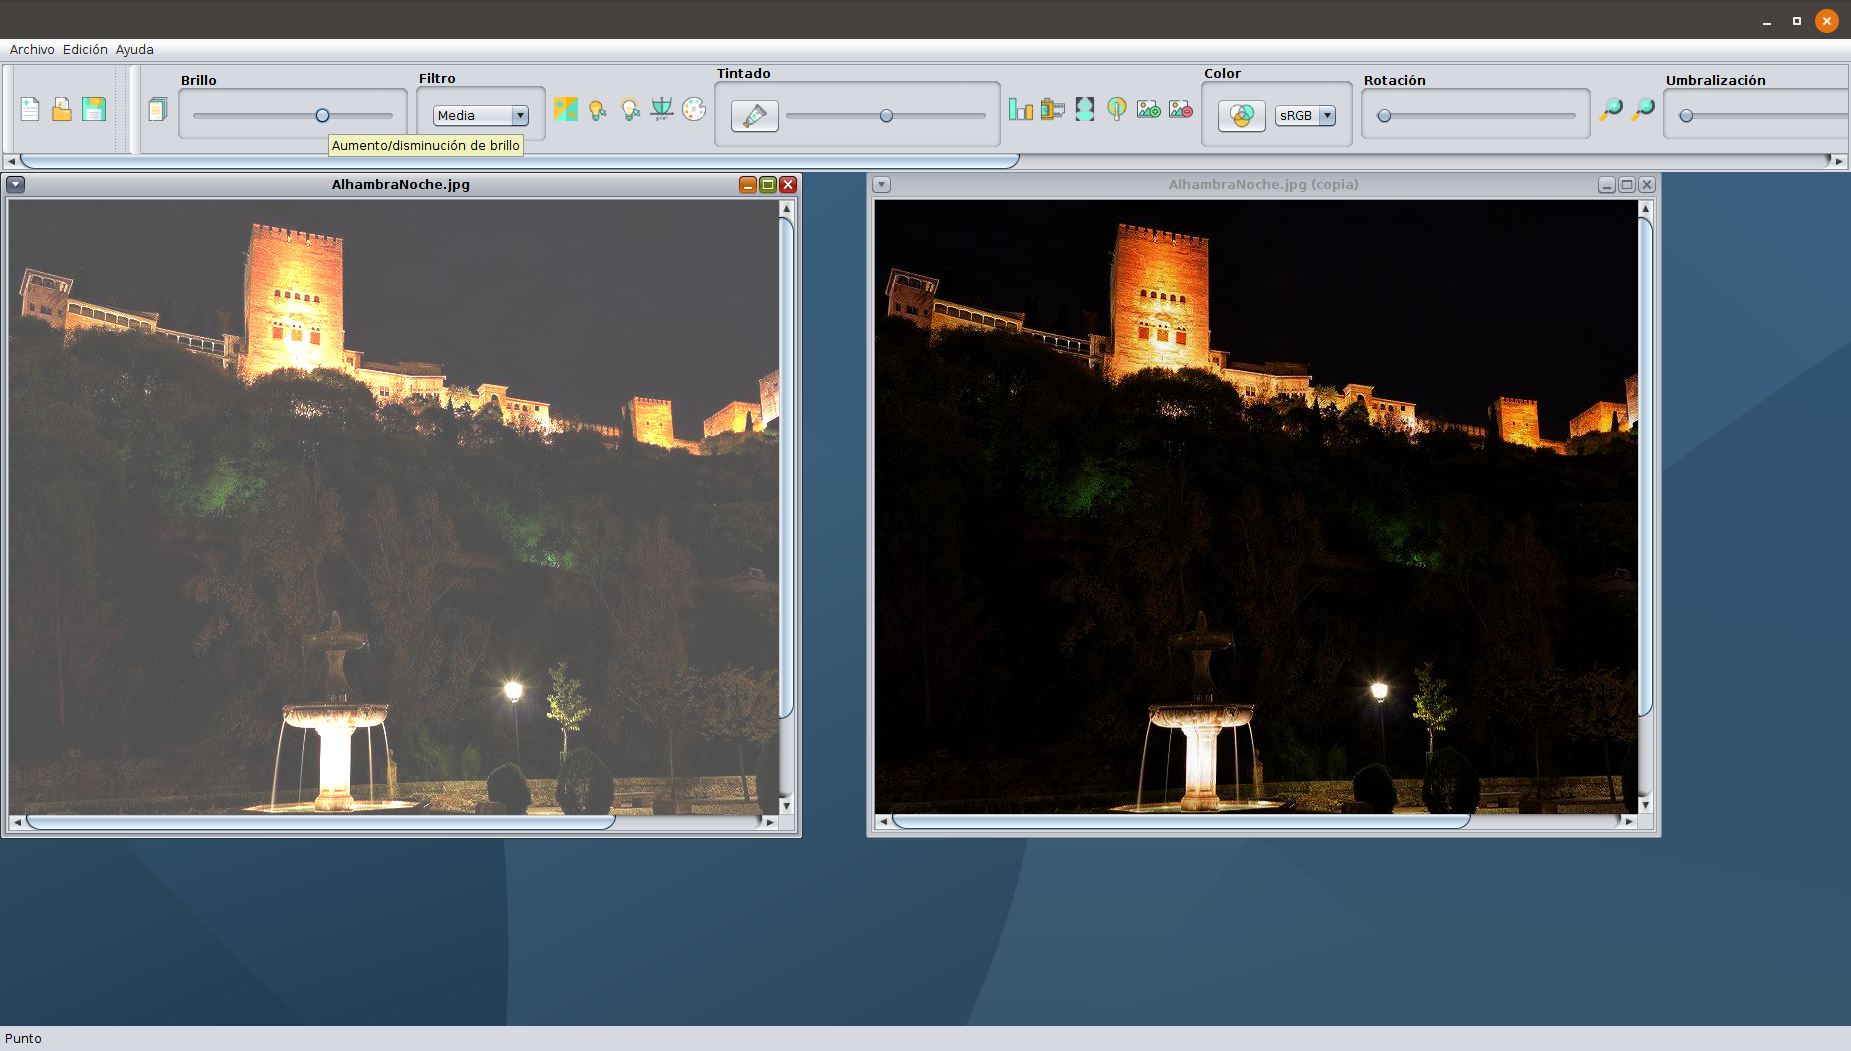
\includegraphics[width=0.6\textwidth]{img/brillo.png}
\end{figure}

\subsubsection{Emborronamiento}
En este caso, se aplica el filtro media 3x3 que emborrona la imagen de manera suave.

\begin{figure}[H]
\centering
	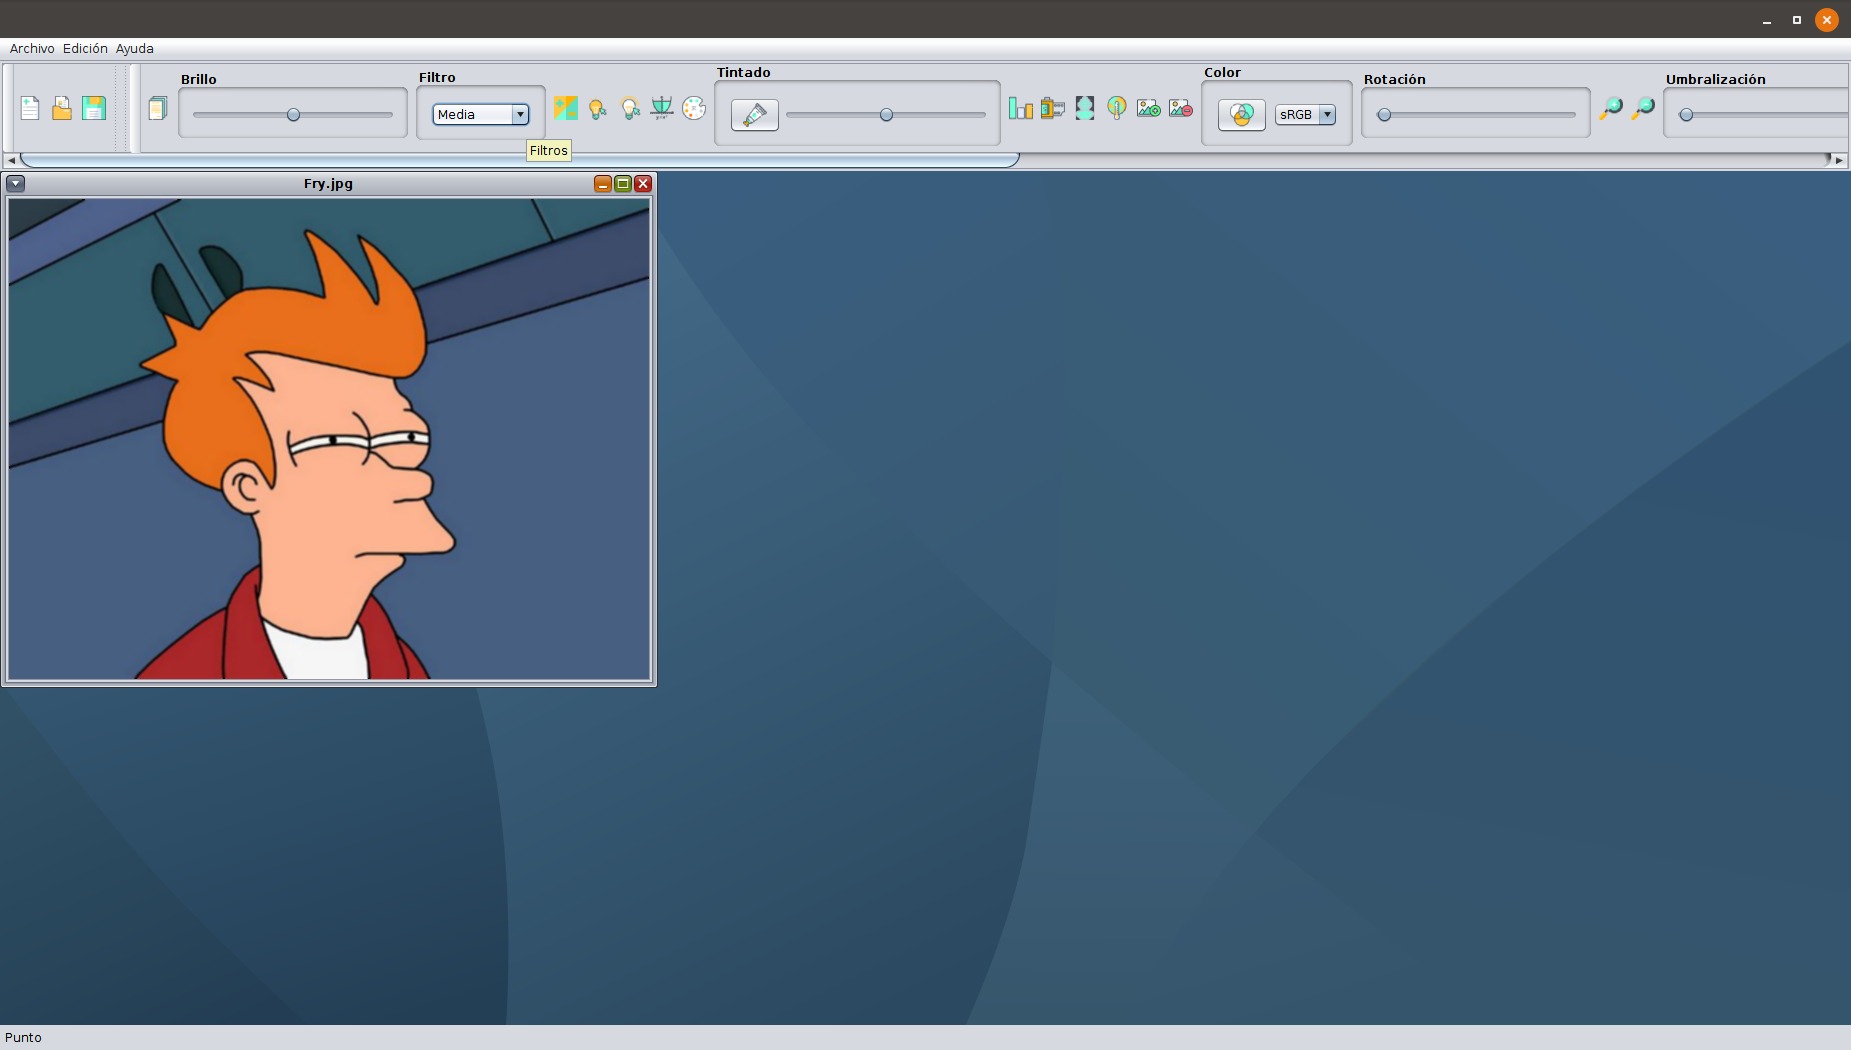
\includegraphics[width=0.6\textwidth]{img/media.png}
\end{figure}

\subsubsection{Enfoque}
Al contrario que el emborronamiento, este filtro permite definir mejor los bordes de la imagen, haciendo que ésta se vea más nítida.

\begin{figure}[H]
\centering
	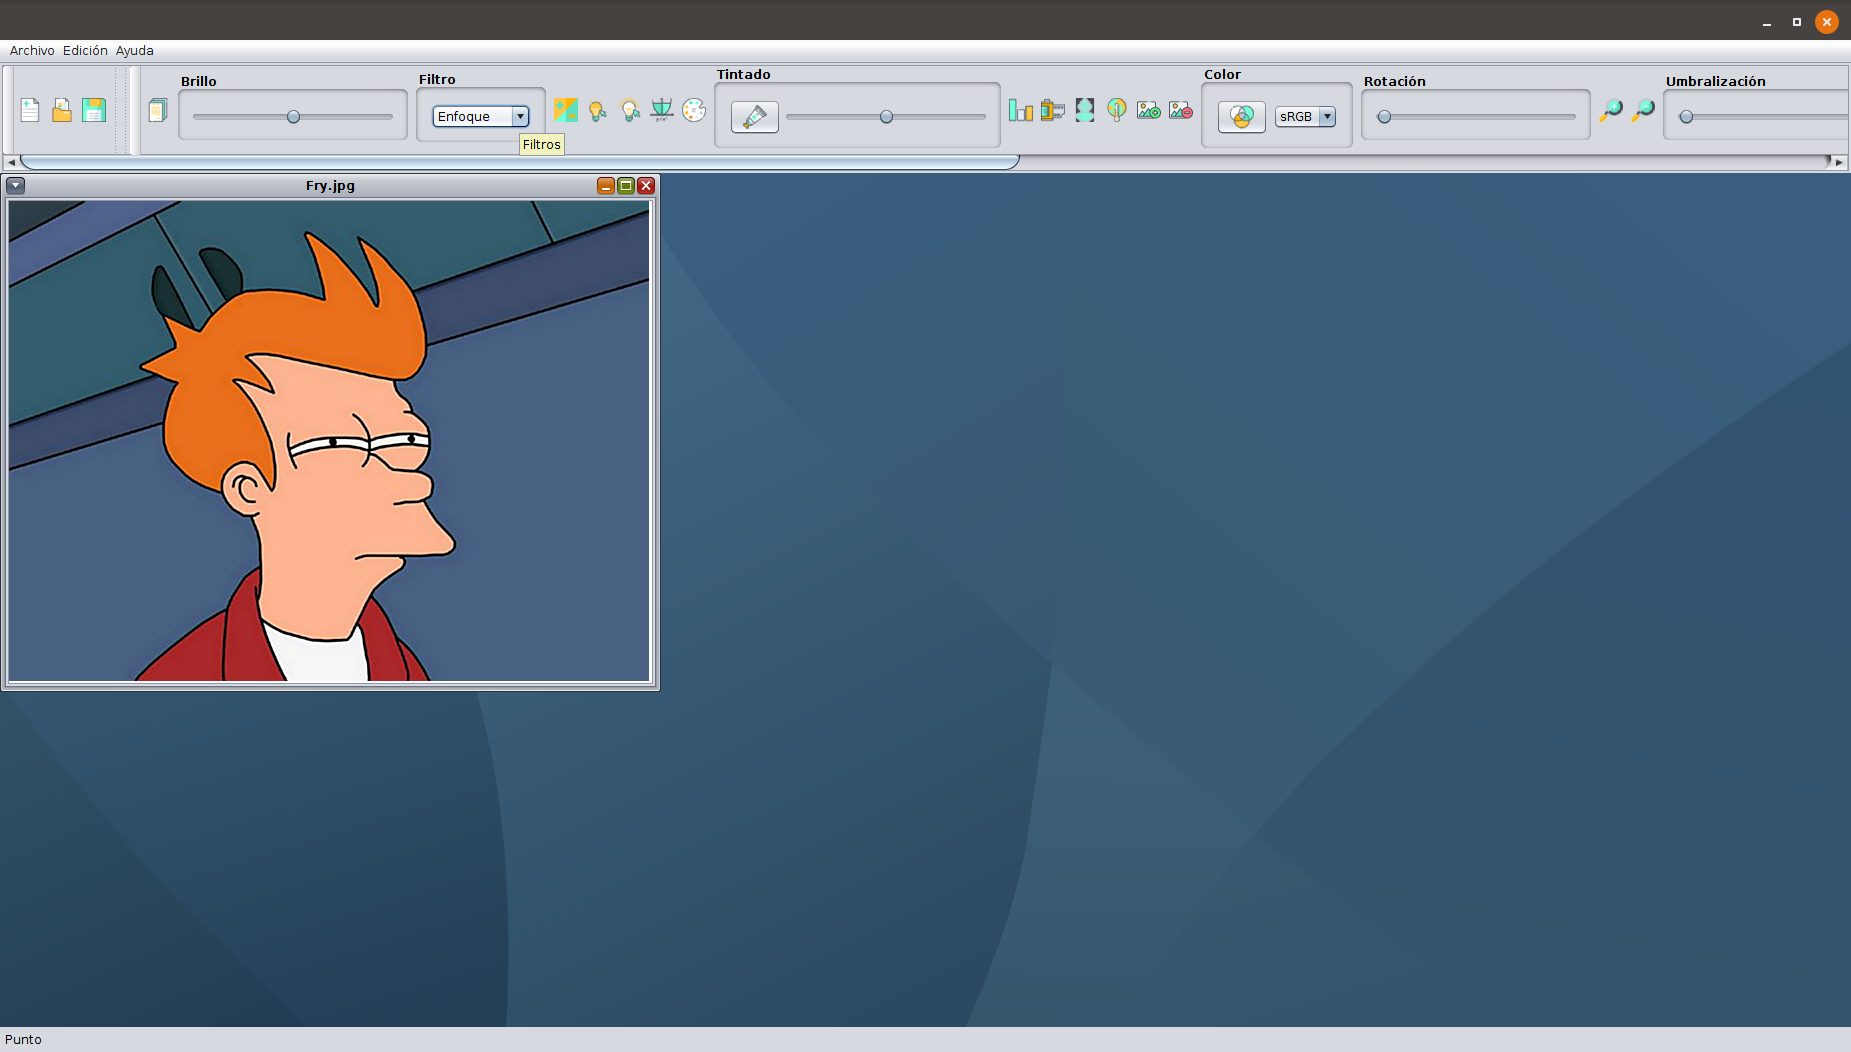
\includegraphics[width=0.6\textwidth]{img/enfoque.png}
\end{figure}

\subsubsection{Relieve}
En este caso, los bordes presentes en la imagen se verán más definidos, dando la impresión de que la imagen está en 3D.

\begin{figure}[H]
\centering
	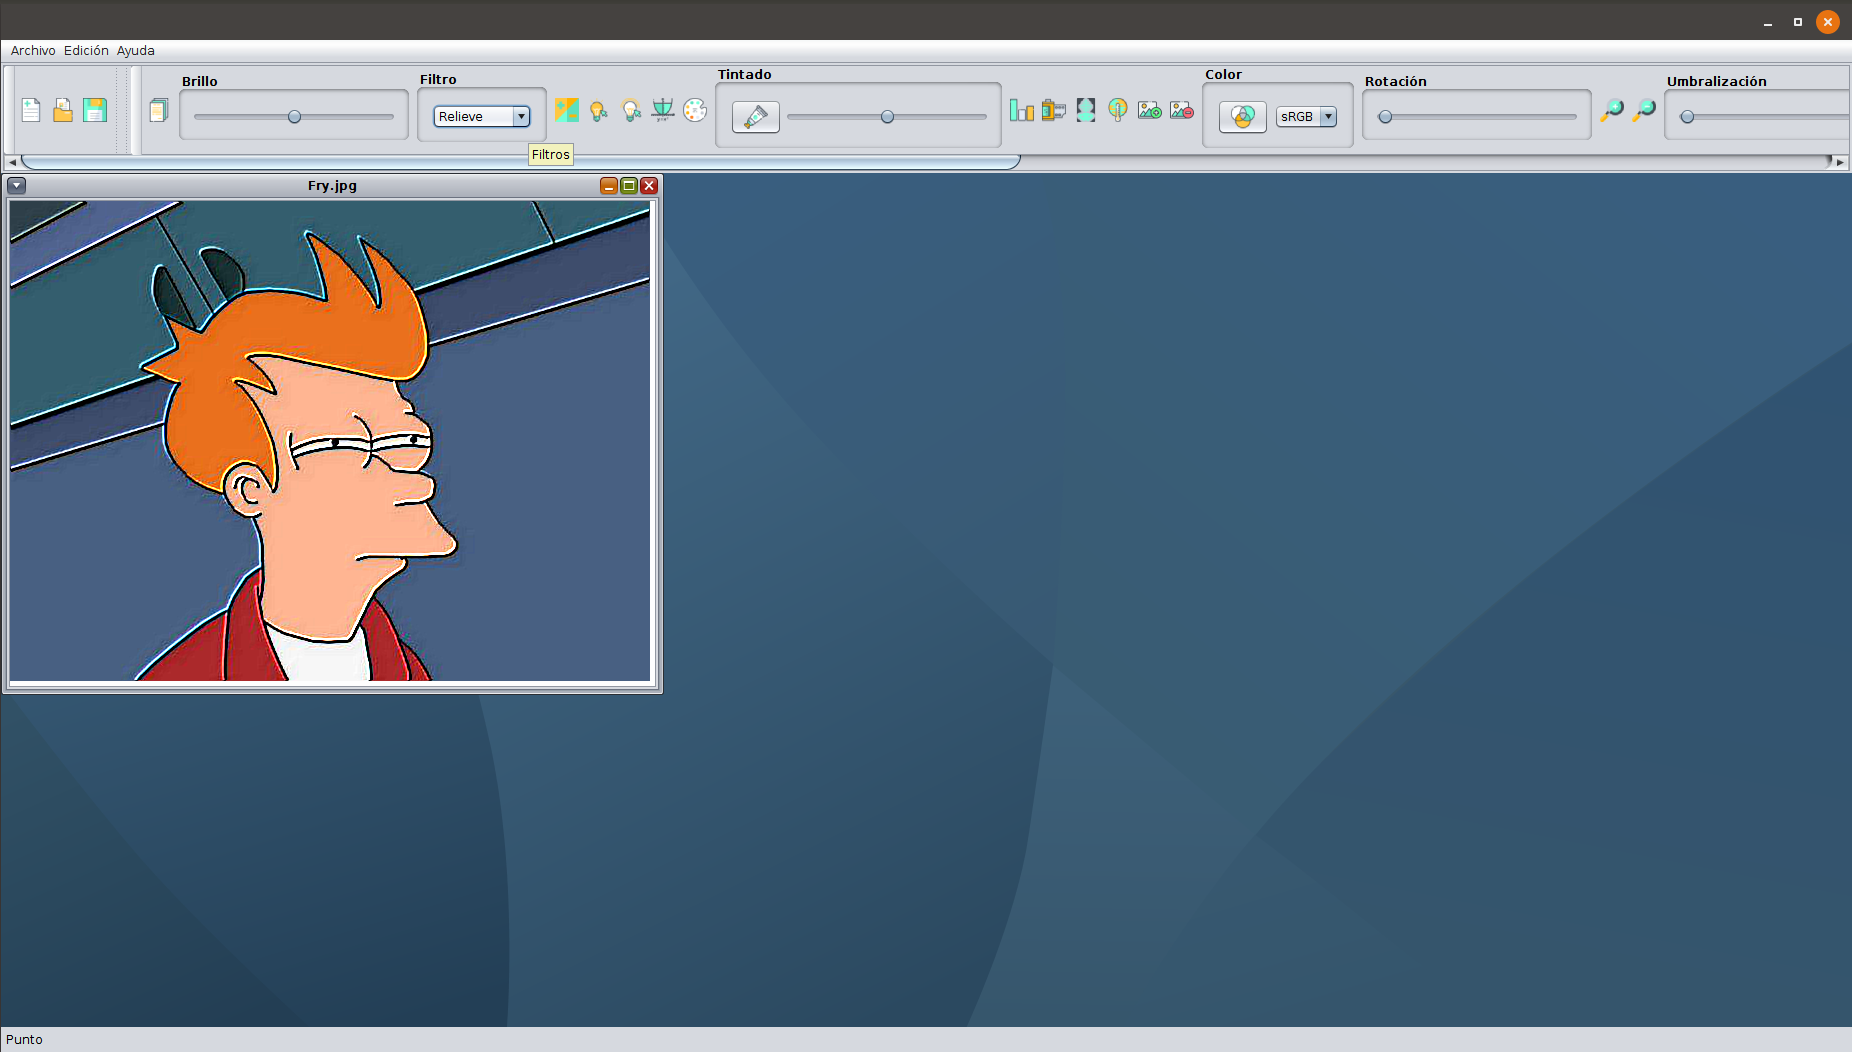
\includegraphics[width=0.6\textwidth]{img/relieve.png}
\end{figure}

\subsubsection{Contraste}
Los pixeles más oscuros acentúan su oscurecimiento y los más claros, se aclaran más.

\begin{figure}[H]
\centering
	
\includegraphics[width=0.6\textwidth]{img/contraste.png}
\end{figure}

\subsubsection{Contraste con iluminación}
Las partes oscuras se aclaran, las claras se mantienen igual, dando un aspecto de mayor luminosidad. Filtro adecuado para imágenes oscuras.

\begin{figure}[H]
\centering
	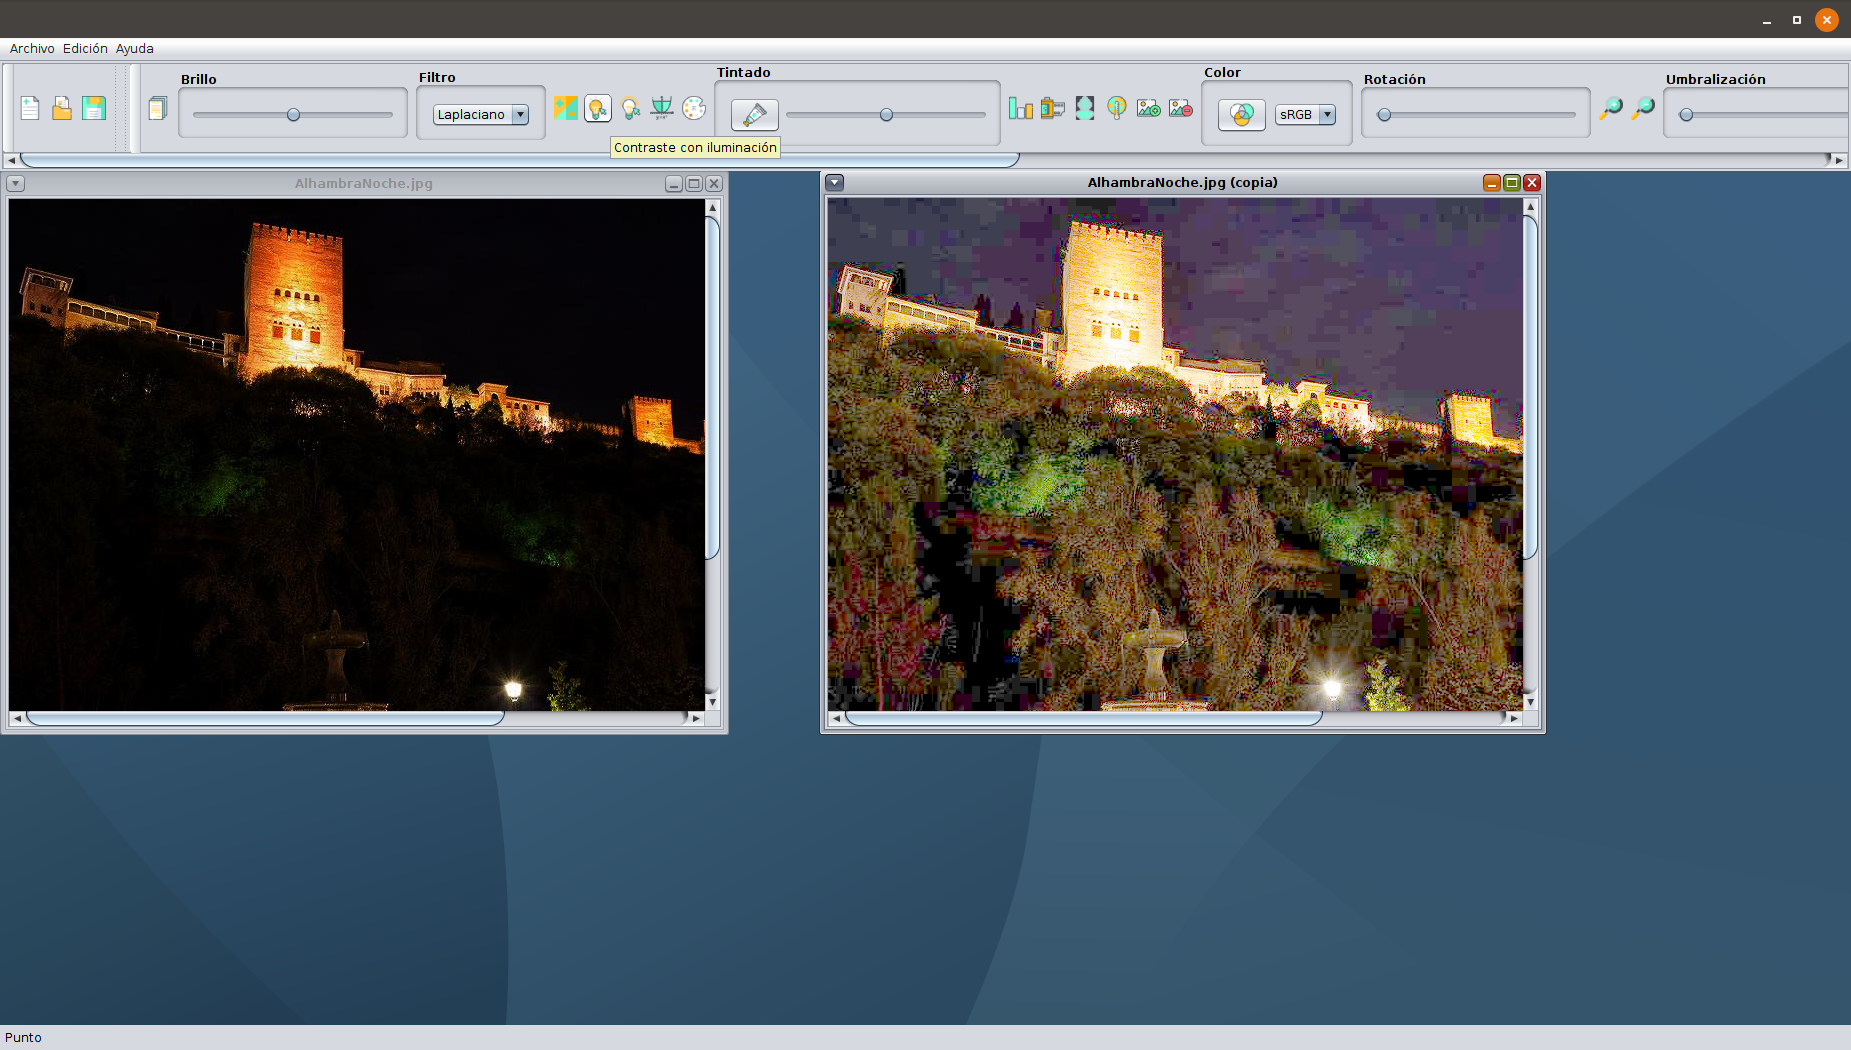
\includegraphics[width=0.6\textwidth]{img/conilu.png}
\end{figure}

\subsubsection{Contraste con oscurecimiento}
A la inversa que el contraste con iluminación; las partes claras se oscurecen y las oscuras se mantienen. Adecuado para imágenes sobreexpuestas.

\begin{figure}[H]
\centering
	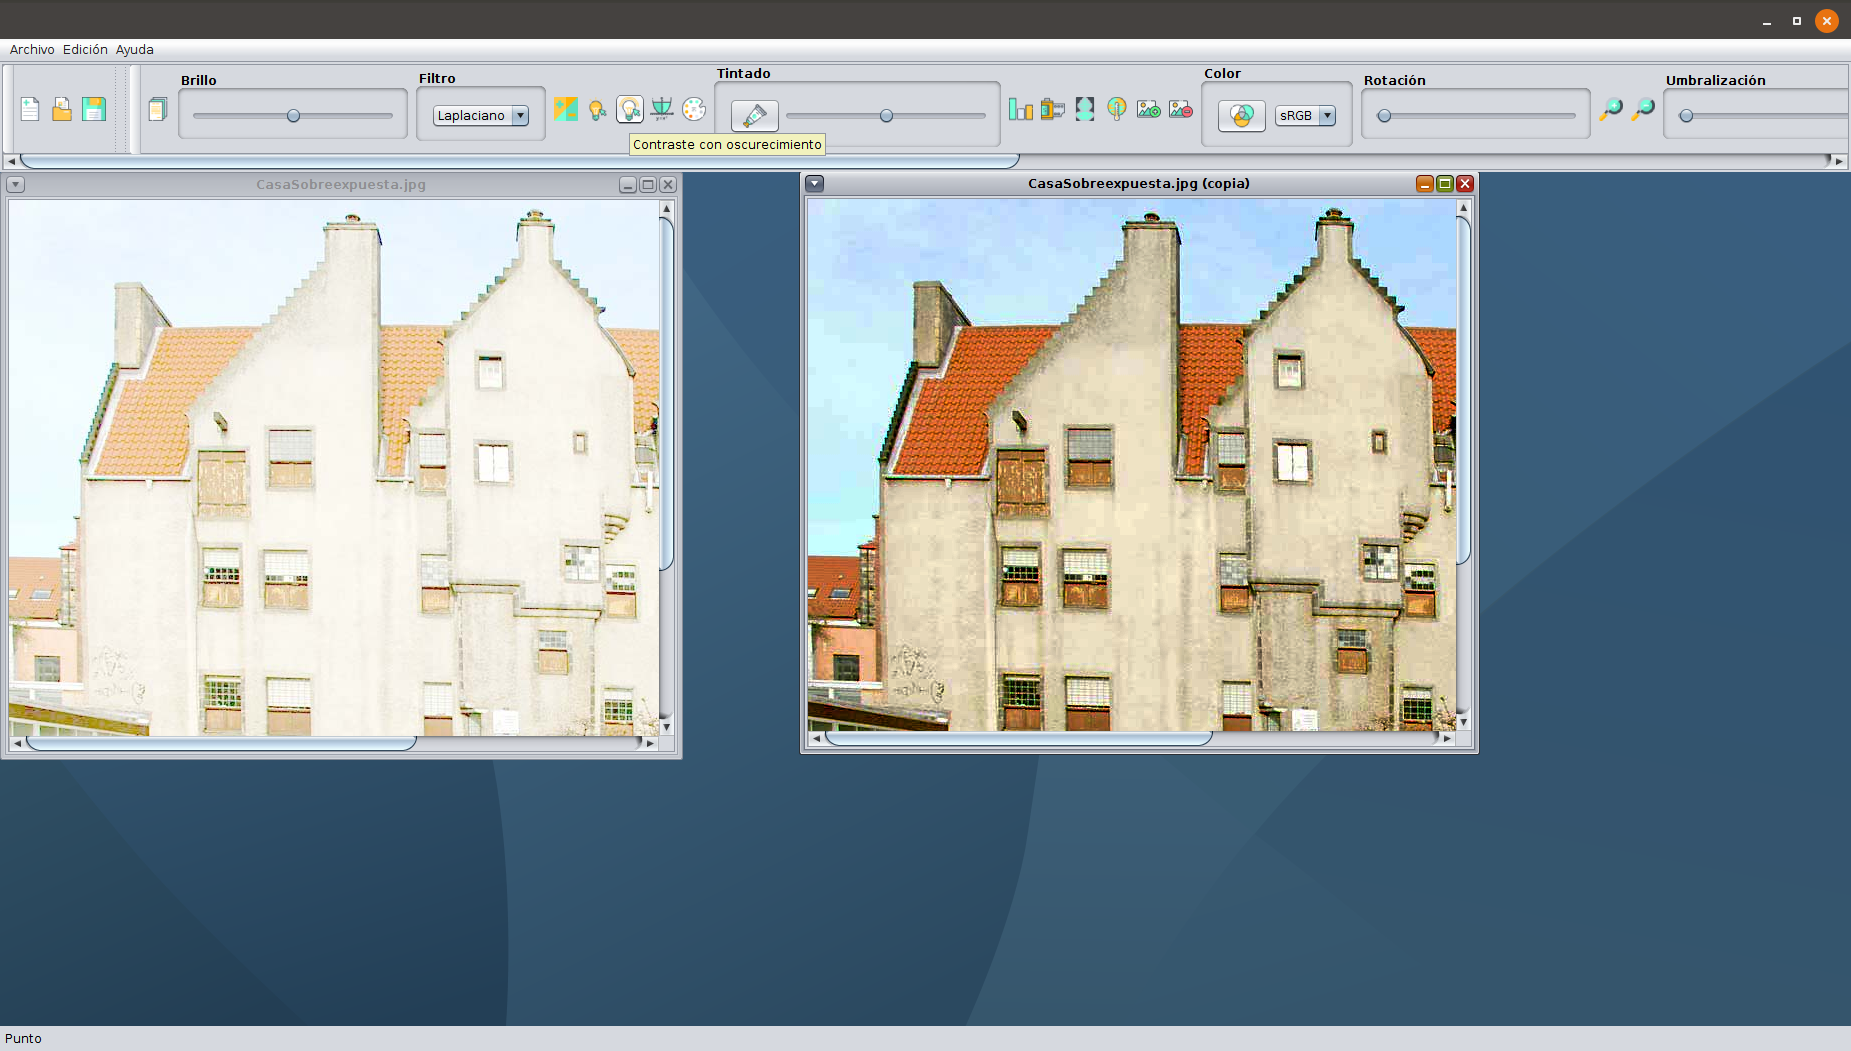
\includegraphics[width=0.6\textwidth]{img/conoscu.png}
\end{figure}

\subsubsection{Negativo}
Los colores de la imagen se invierten. En este caso, he utilizado la función ya implementada en el paquete \textsc{sm.image}, de forma que solo he hecho la aplicación de dicha función, no la manera de tratar los pixeles de la imagen para conseguir el efecto.

\begin{figure}[H]
\centering
	
\includegraphics[width=0.6\textwidth]{img/negativo.png}
\end{figure}

\subsubsection{Extracción de bandas y espacios de color}
Se muestran dos funcionalidades en una: se convierten las imágenes a distintos espacios de color y, si es posible, se extraen sus bandas:
	\begin{itemize}
		\item Conversión a RGB y extracción de bandas.
			\begin{figure}[H]
			\centering
				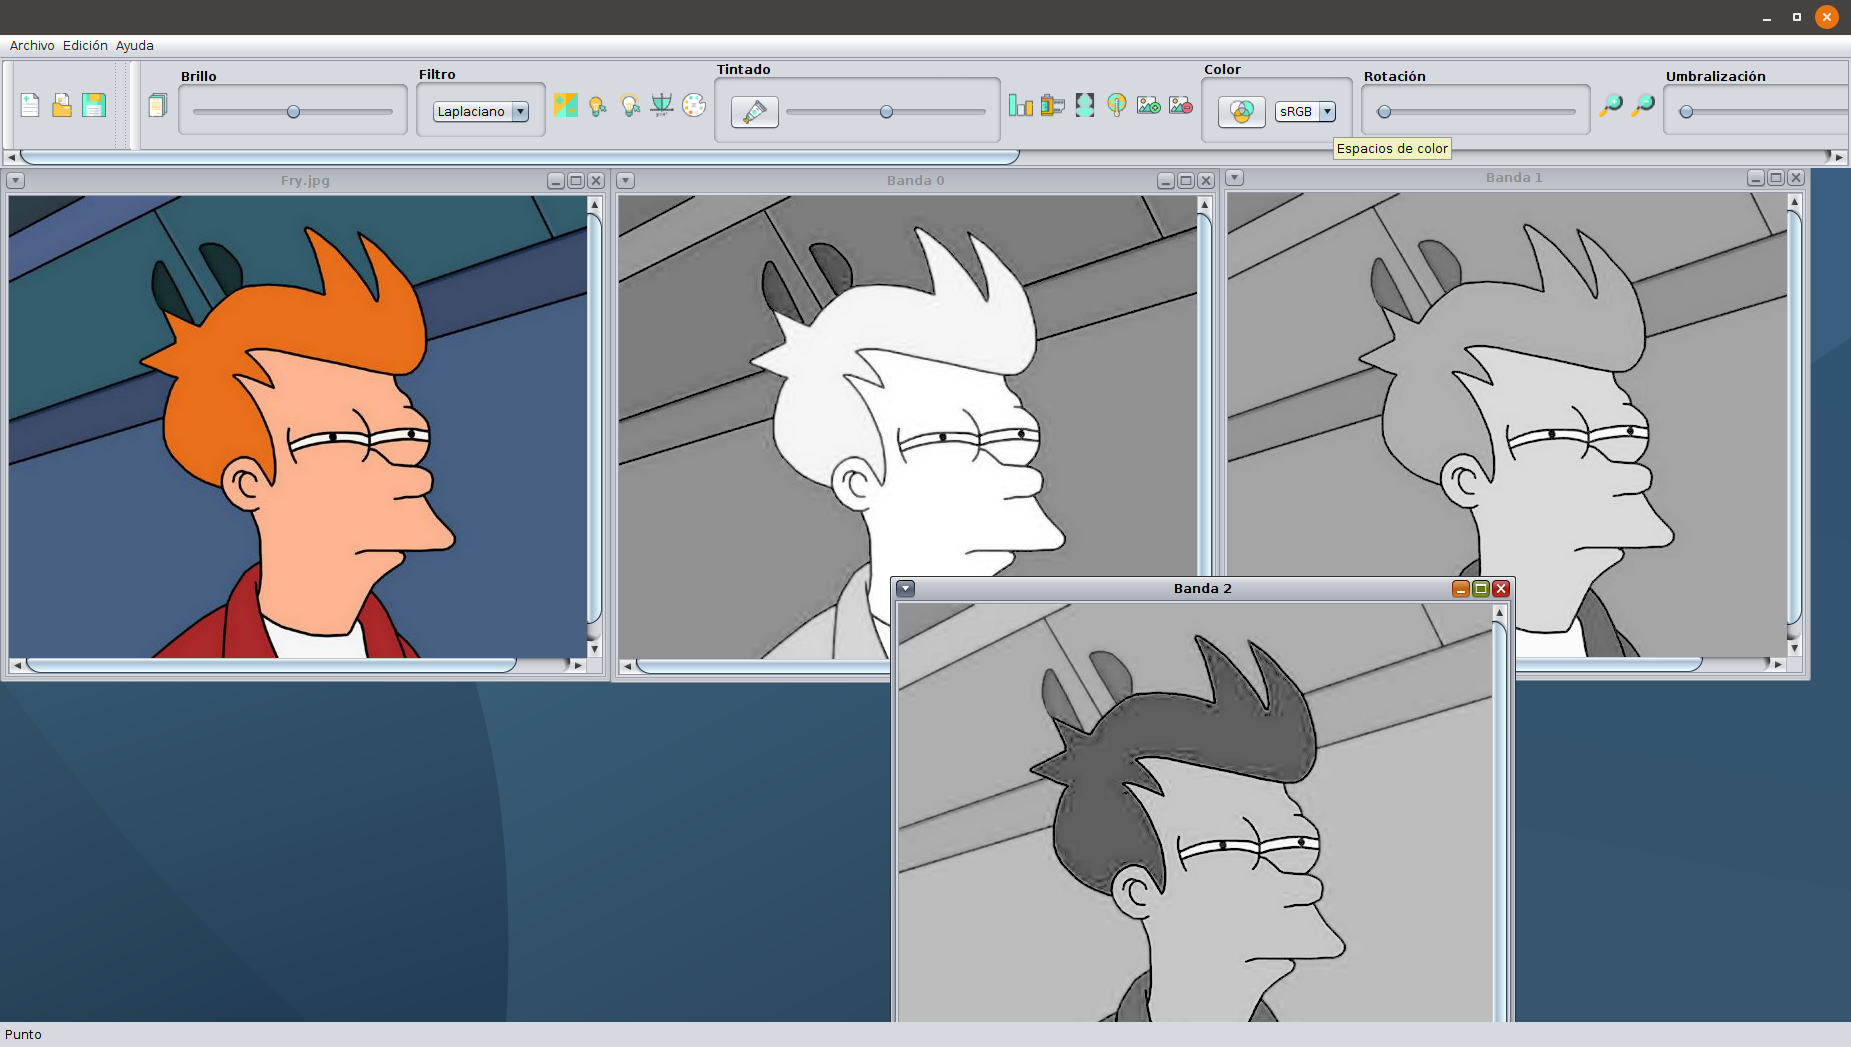
\includegraphics[width=0.7\textwidth]{img/bandasrgb.png}
			\end{figure}
		\item Conversión a YCC y extracción de bandas.
			\begin{figure}[H]
			\centering
				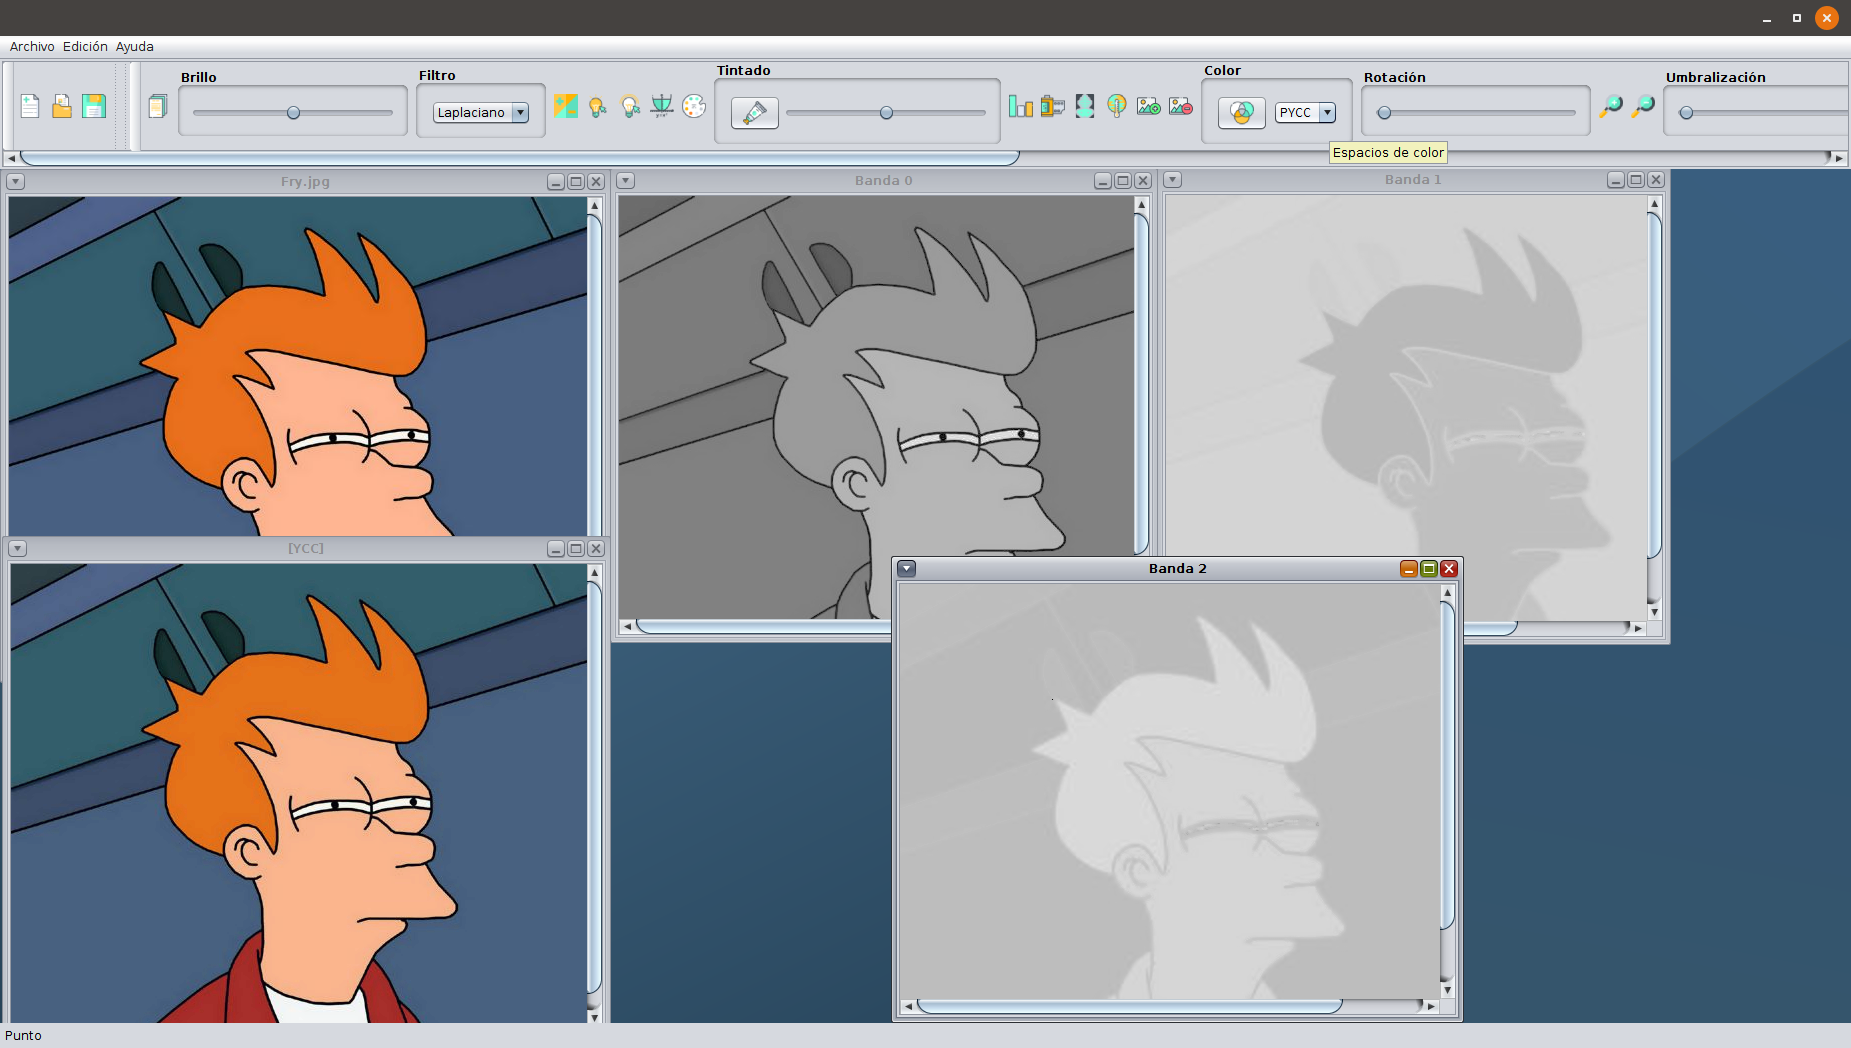
\includegraphics[width=0.7\textwidth]{img/bandasycc.png}
			\end{figure}
		\item Conversión a GRAY.
			\begin{figure}[H]
			\centering
				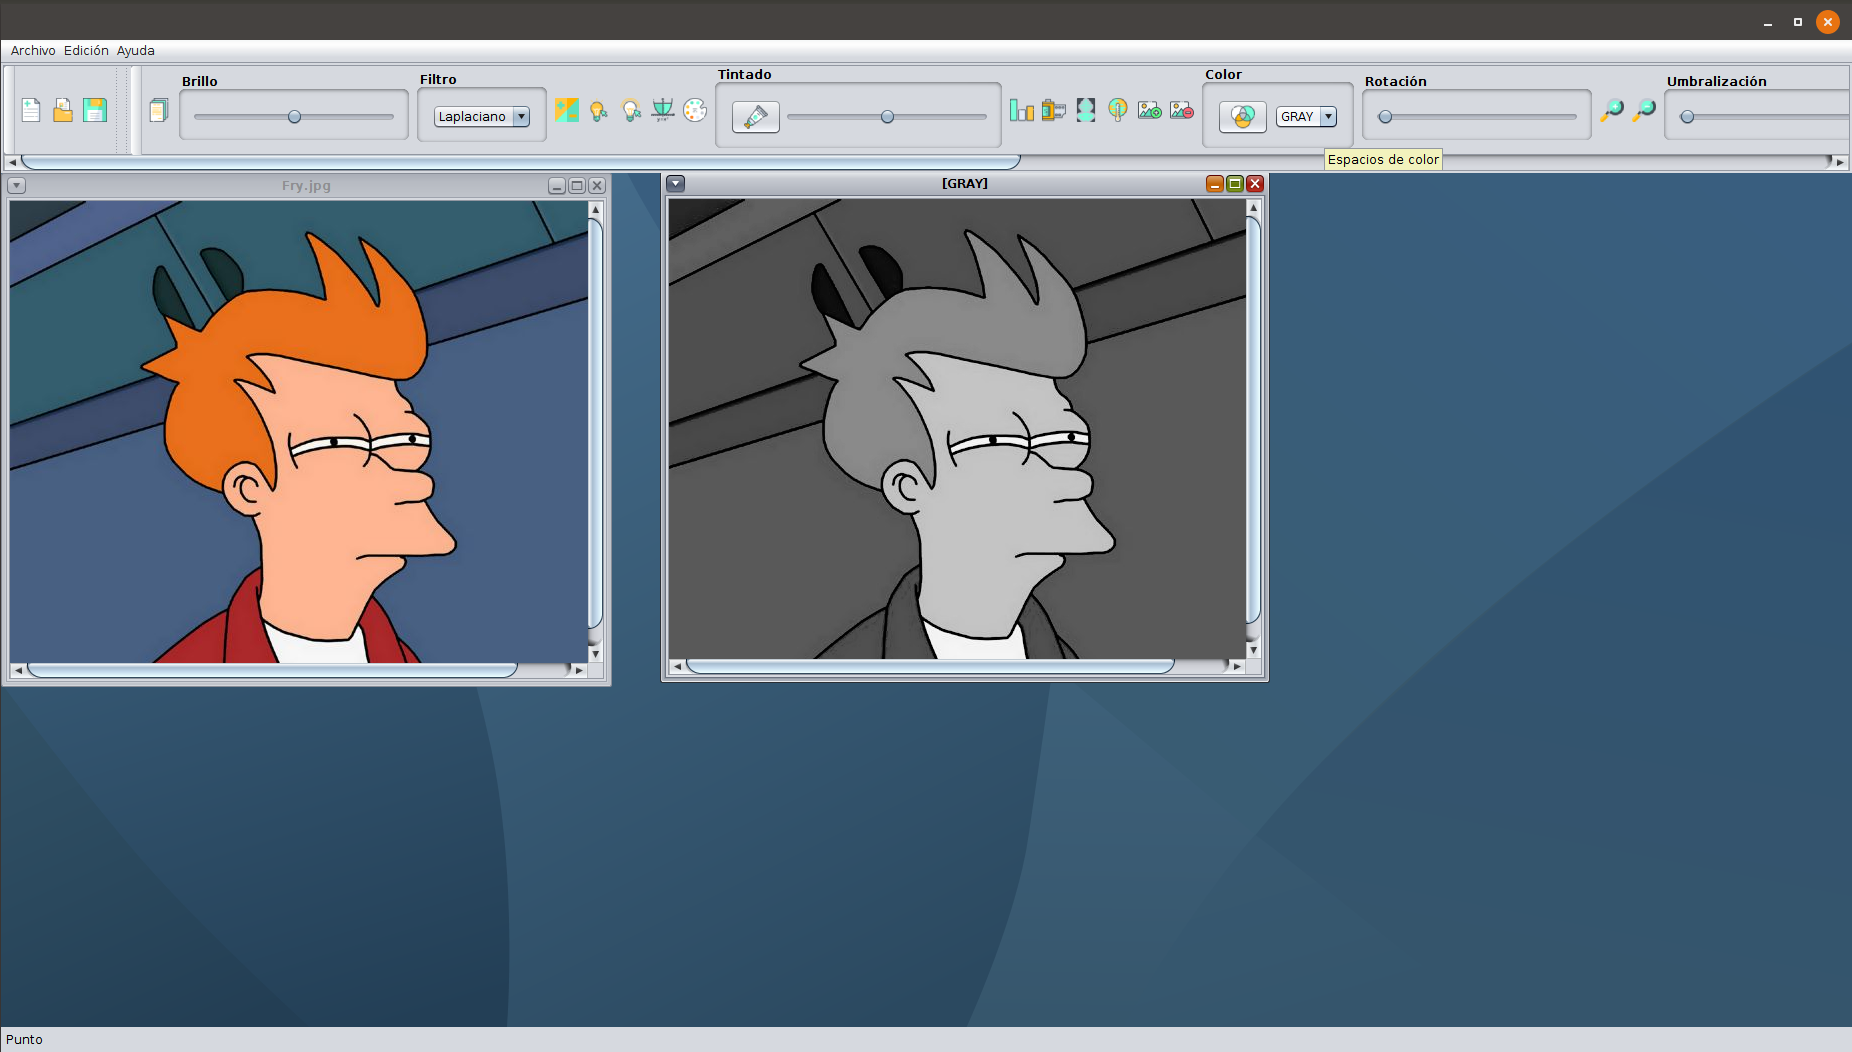
\includegraphics[width=0.7\textwidth]{img/gray.png}
			\end{figure}
	\end{itemize}
	
\subsubsection{Rotación}
La imagen rota mediante un deslizador en 360º.

\begin{figure}[H]
\centering
	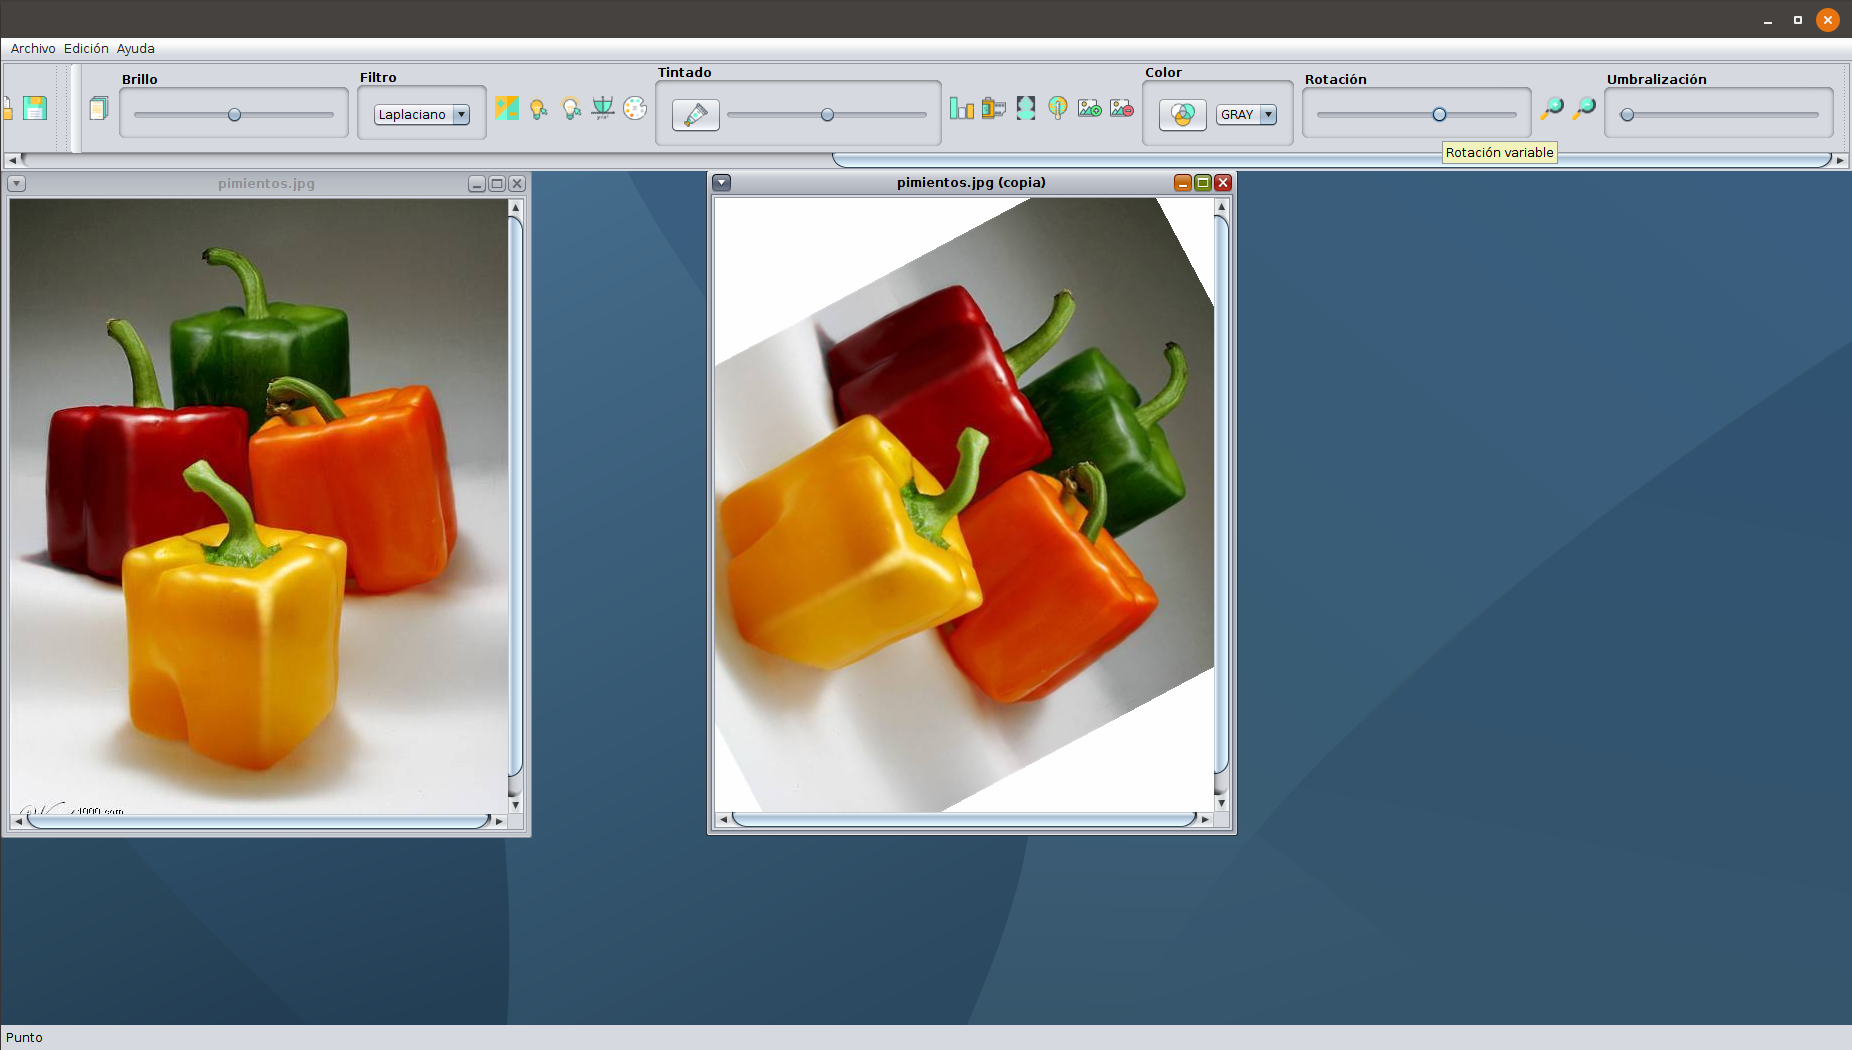
\includegraphics[width=0.6\textwidth]{img/rotar.png}
\end{figure}

\subsubsection{Zoom-in}
Se aumenta el tamaño de la imagen pero sin producir un recorte para ajustarse a la ventana. La imagen se mantiene íntegra.

\begin{figure}[H]
\centering
	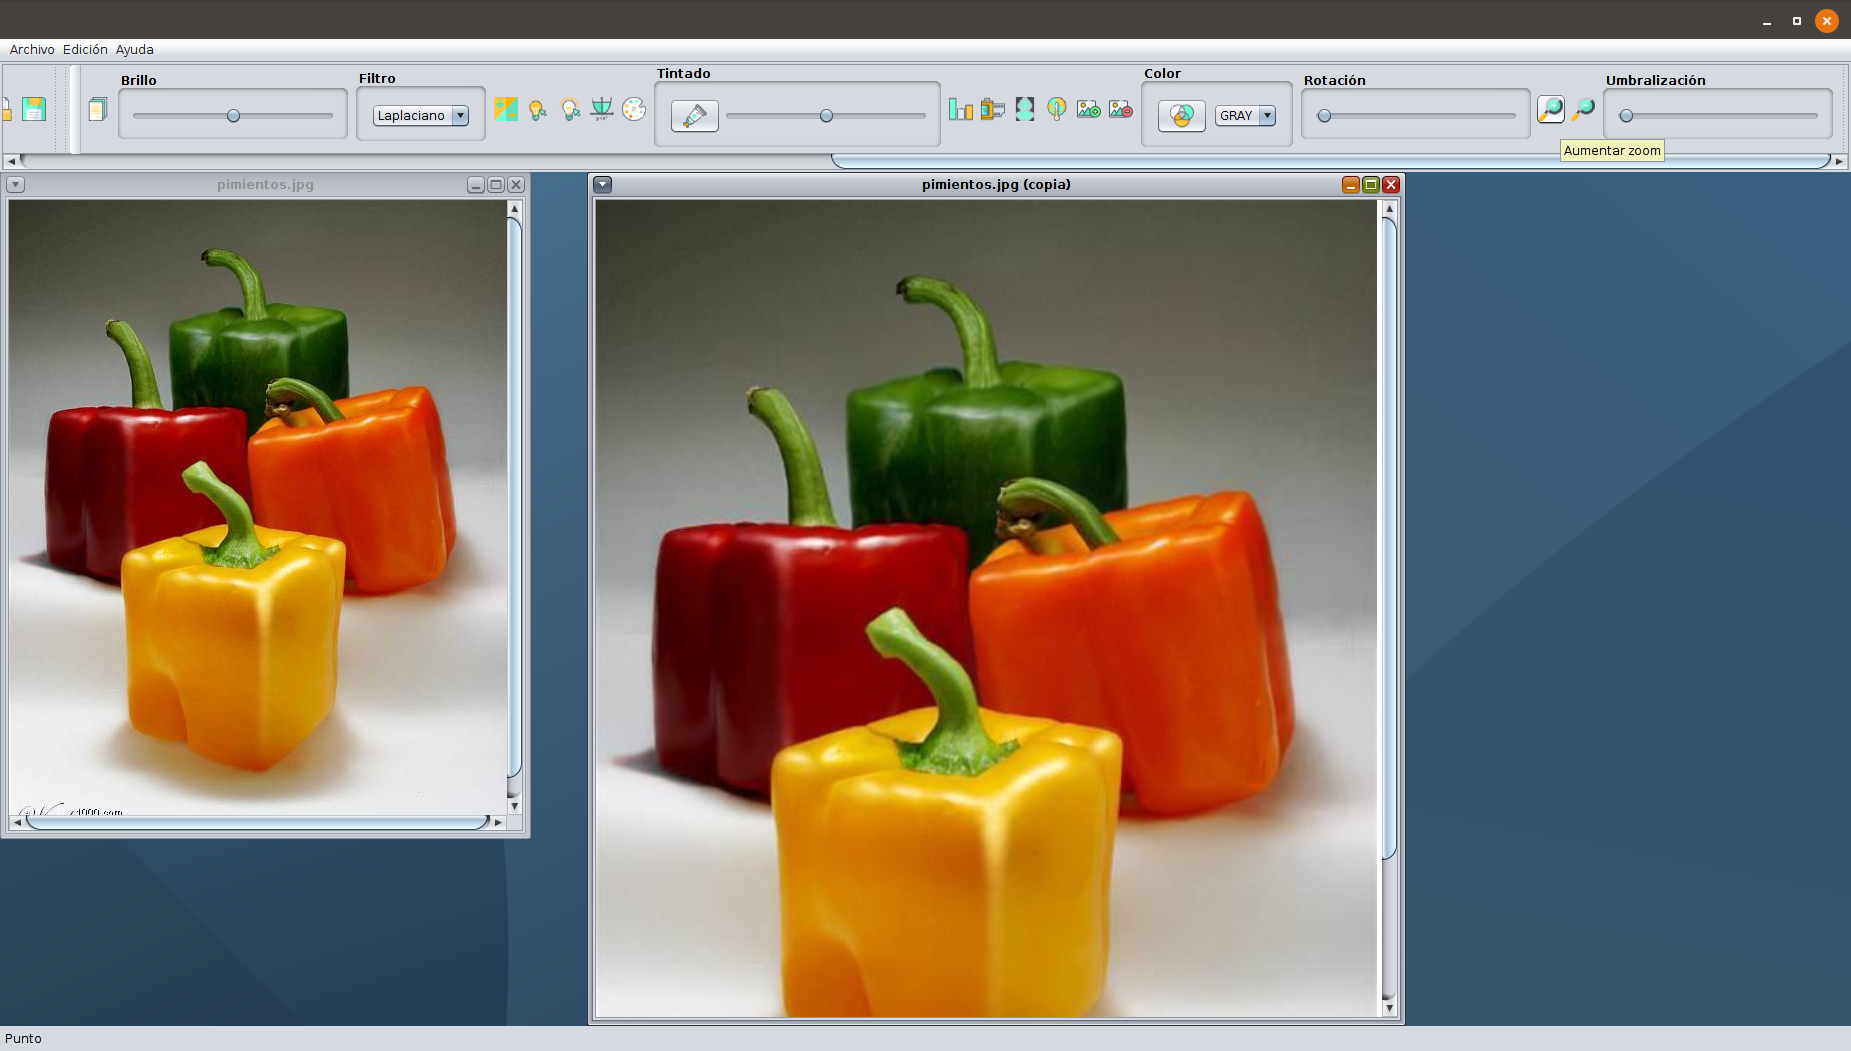
\includegraphics[width=0.6\textwidth]{img/escalamas.png}
\end{figure}

\subsubsection{Zoom-out}
Se disminuye la imagen pero sin añadir marco o borde a la imagen original.

\begin{figure}[H]
\centering
	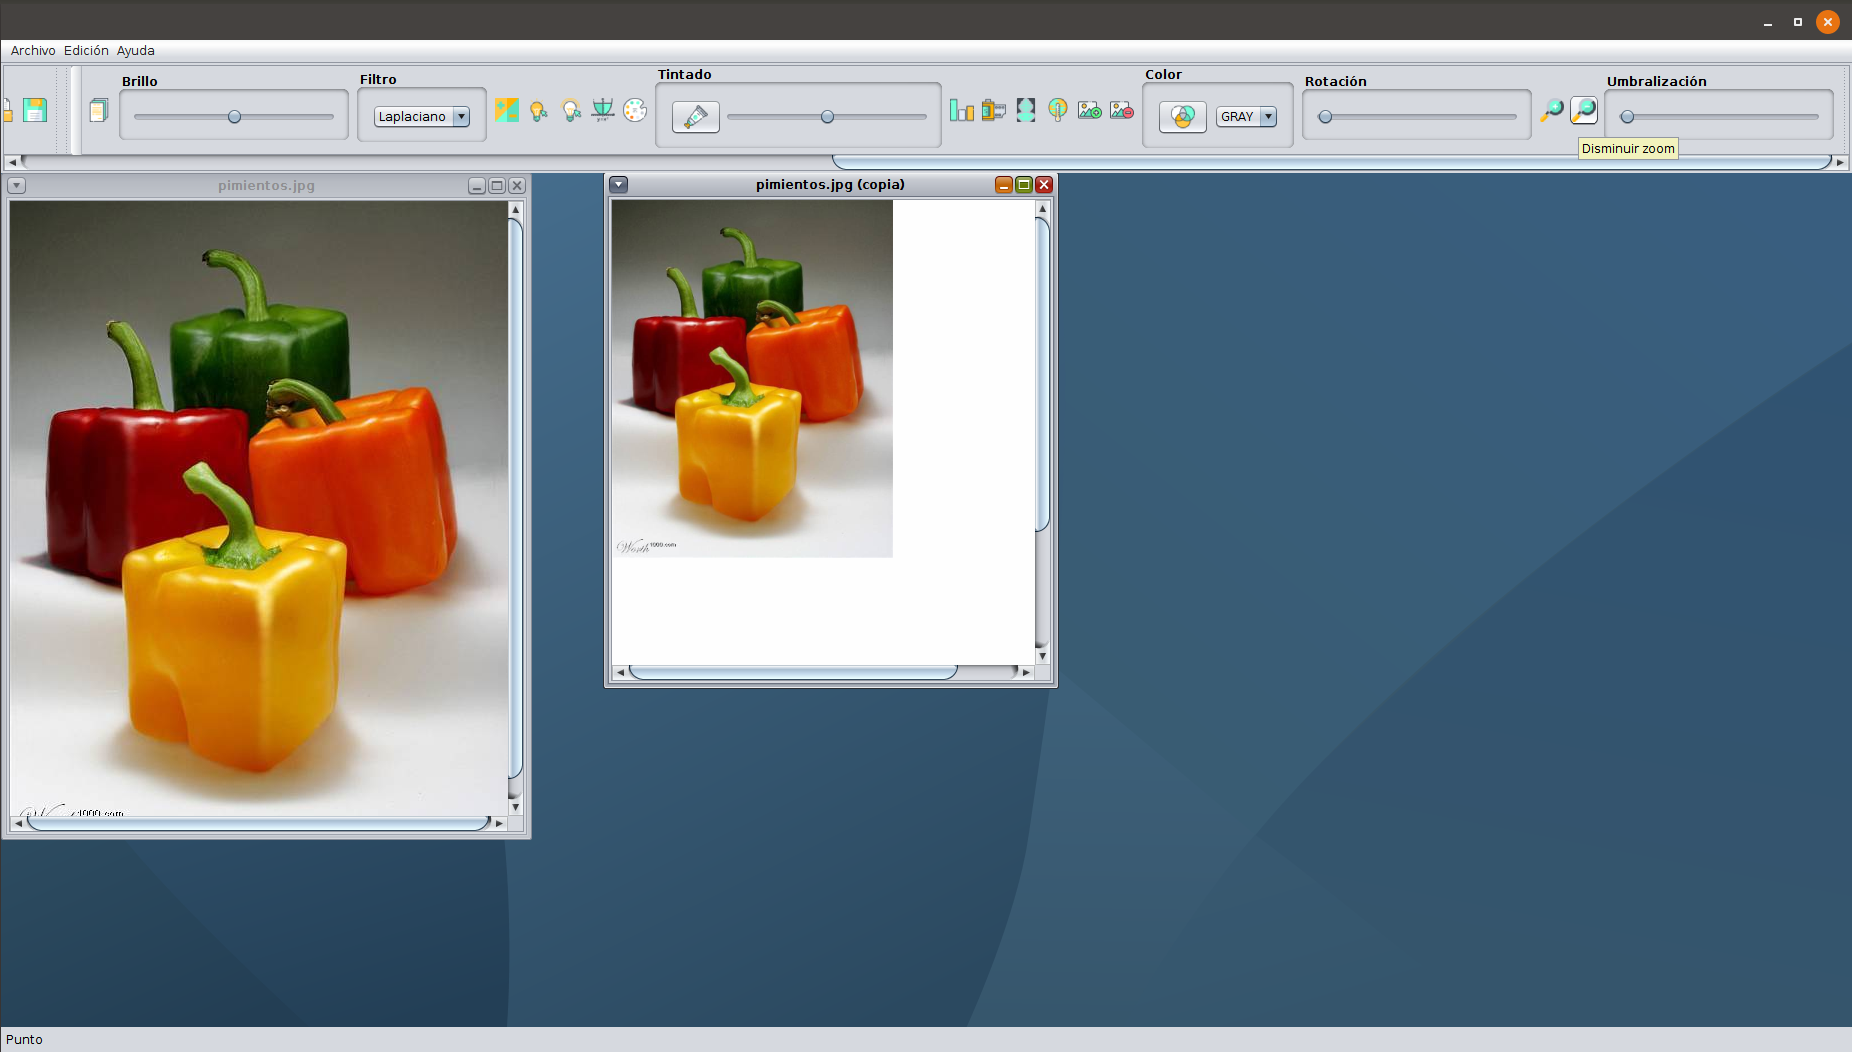
\includegraphics[width=0.6\textwidth]{img/escalamenos.png}
\end{figure}

\subsubsection{Tintado (mediante botón)}
Se aplica el tinte del color elegido con una potencia de 0,5.

\begin{figure}[H]
\centering
	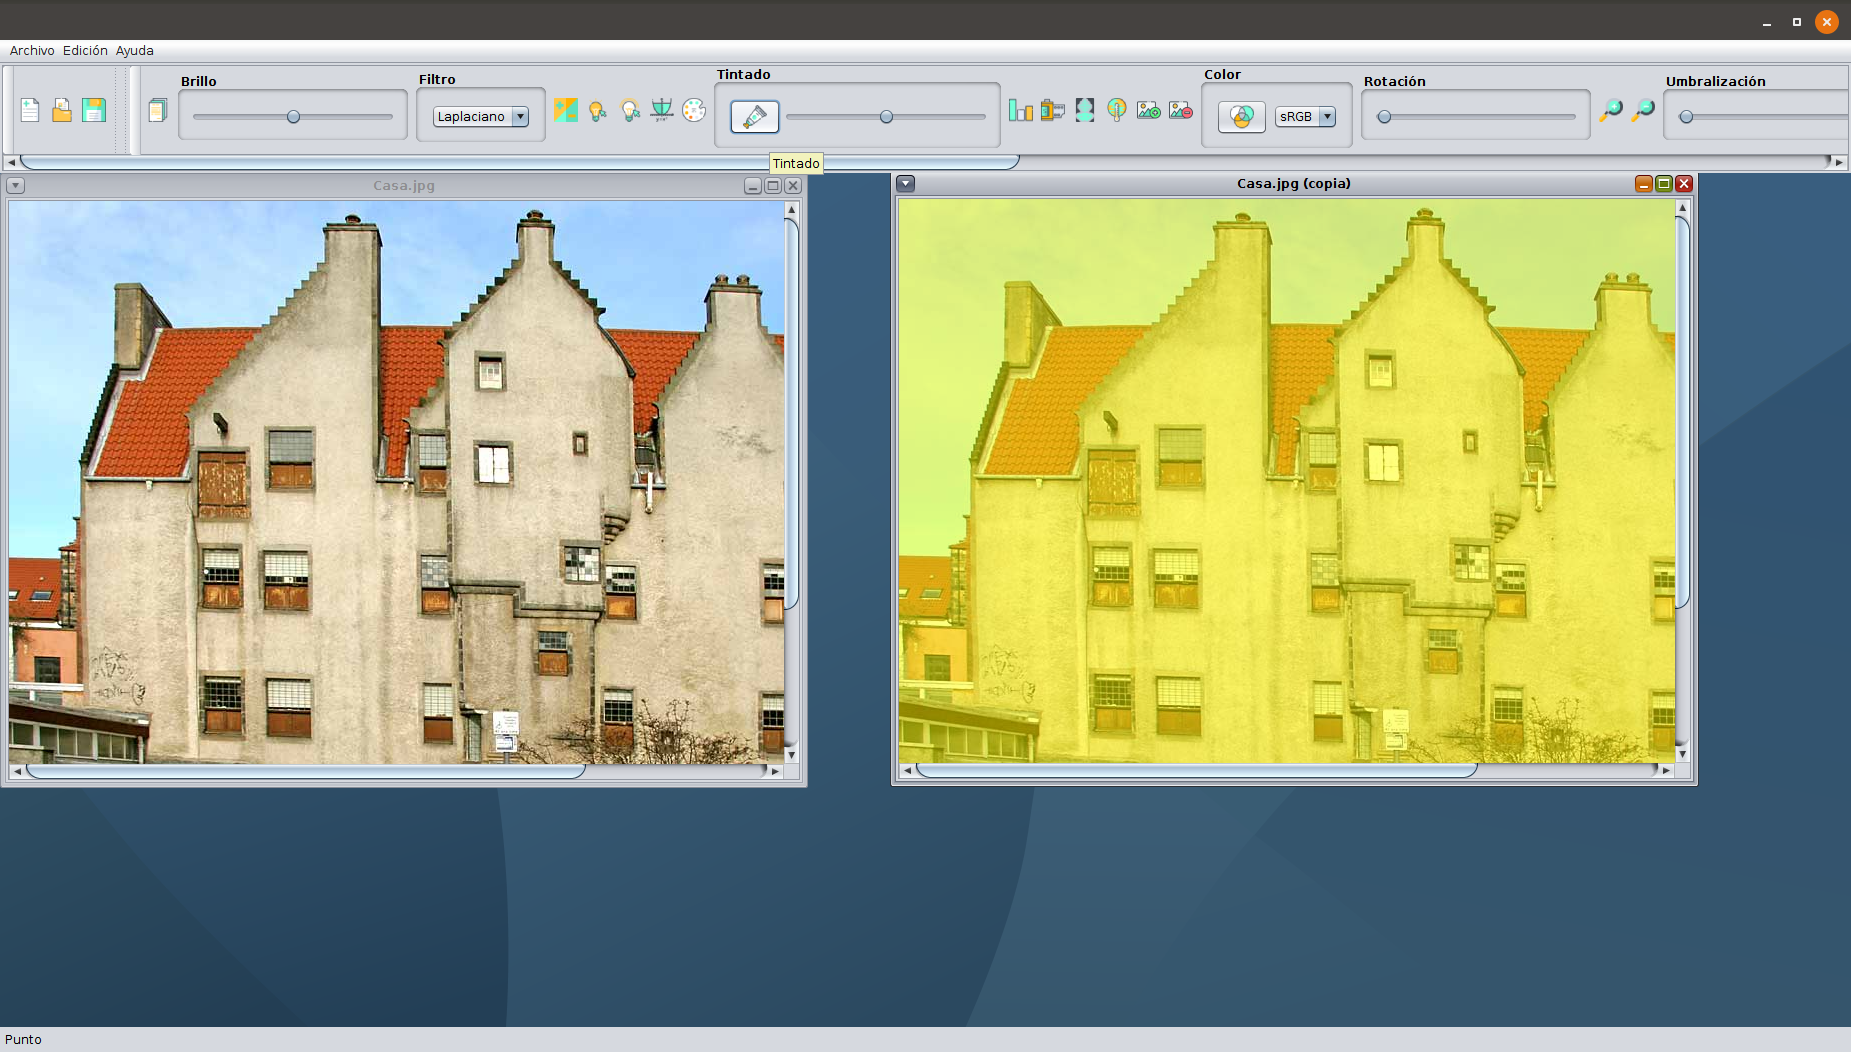
\includegraphics[width=0.6\textwidth]{img/tinte.png}
\end{figure}

\subsubsection{Ecualización}
Se intenta aclarar la imagen de forma que sea más nítida y se reconozcan mejor las figuras.

\begin{figure}[H]
\centering
	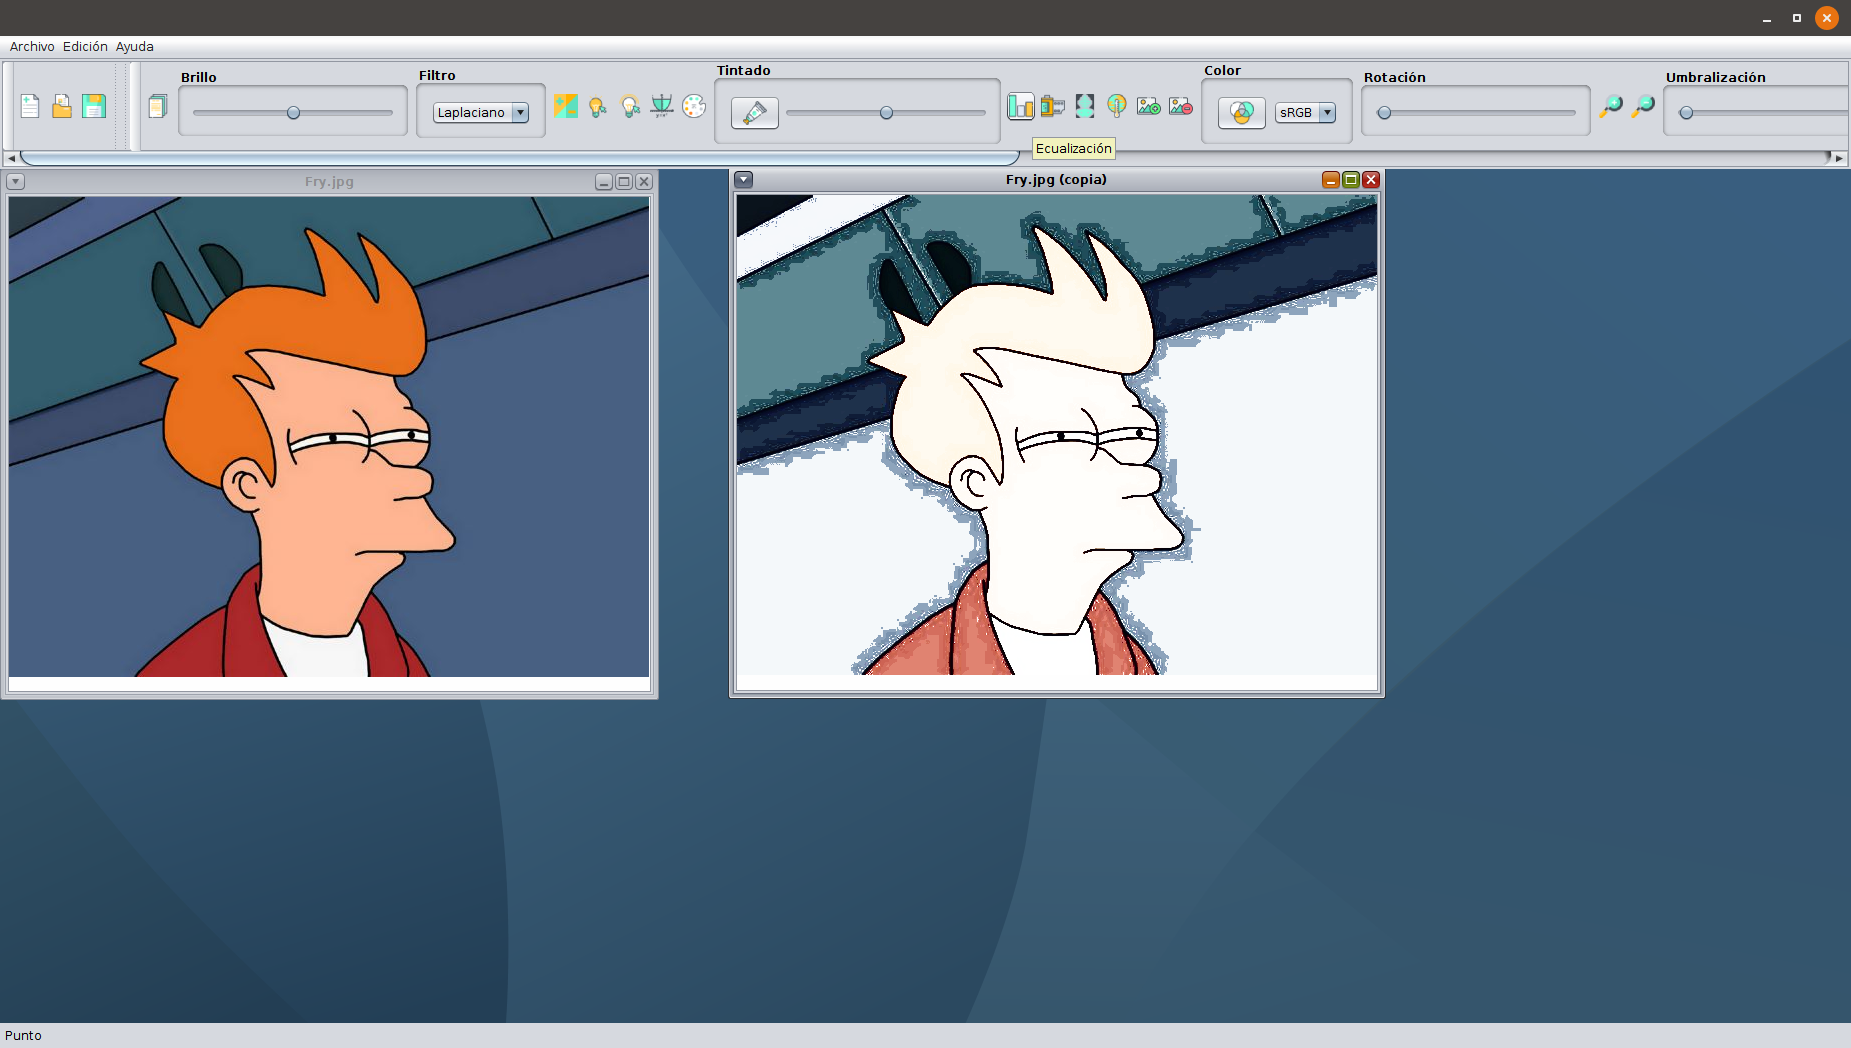
\includegraphics[width=0.6\textwidth]{img/ecual.png}
\end{figure}

\subsubsection{Sepia}
Filtro que da aspecto de imagen antigua. Para ello, se ha definido la clase \textsc{SepiaOp} en el paquete \textsc{sm.ngr.image}. Es una operación pixel a pixel, puesto que hacen falta las tres componentes de la imagen para dar lugar al color final de cada pixel, siguiendo la regla:\\

\begin{lstlisting}
		pixel_comp[0] = (int)(pixel[r]*0.393 + pixel[g]*0.769 + pixel[b]*0.189);
    pixel_comp[1] = (int)(pixel[r]*0.349 + pixel[g]*0.686 + pixel[b]*0.168);
    pixel_comp[2] = (int)(pixel[r]*0.272 + pixel[g]*0.534 + pixel[b]*0.131);
\end{lstlisting}

donde \textsc{r} es la componente roja del pixel, \textsc{g} la verde y \textsc{b} la azul.\\

Un ejemplo de funcionamiento es el siguiente:

\begin{figure}[H]
\centering
	
\includegraphics[width=0.6\textwidth]{img/sepia.png}
\end{figure}

\subsubsection{Umbralización}
En este caso, la imagen de salida es una imagen binaria, donde solo hay blanco o negro, dependiendo del umbral que se imponga. Dicho umbral estará definido por el usuario mediante el deslizador y varía entre 0 y 255.\\

Para poder generar la imagen, se calcula la media de la suma de las tres componentes de cada pixel; si está por debajo del umbral, esa zona queda negra. Si está por encima, en blanco.\\

Un ejemplo de uso sería el siguiente:

\begin{figure}[H]
\centering
	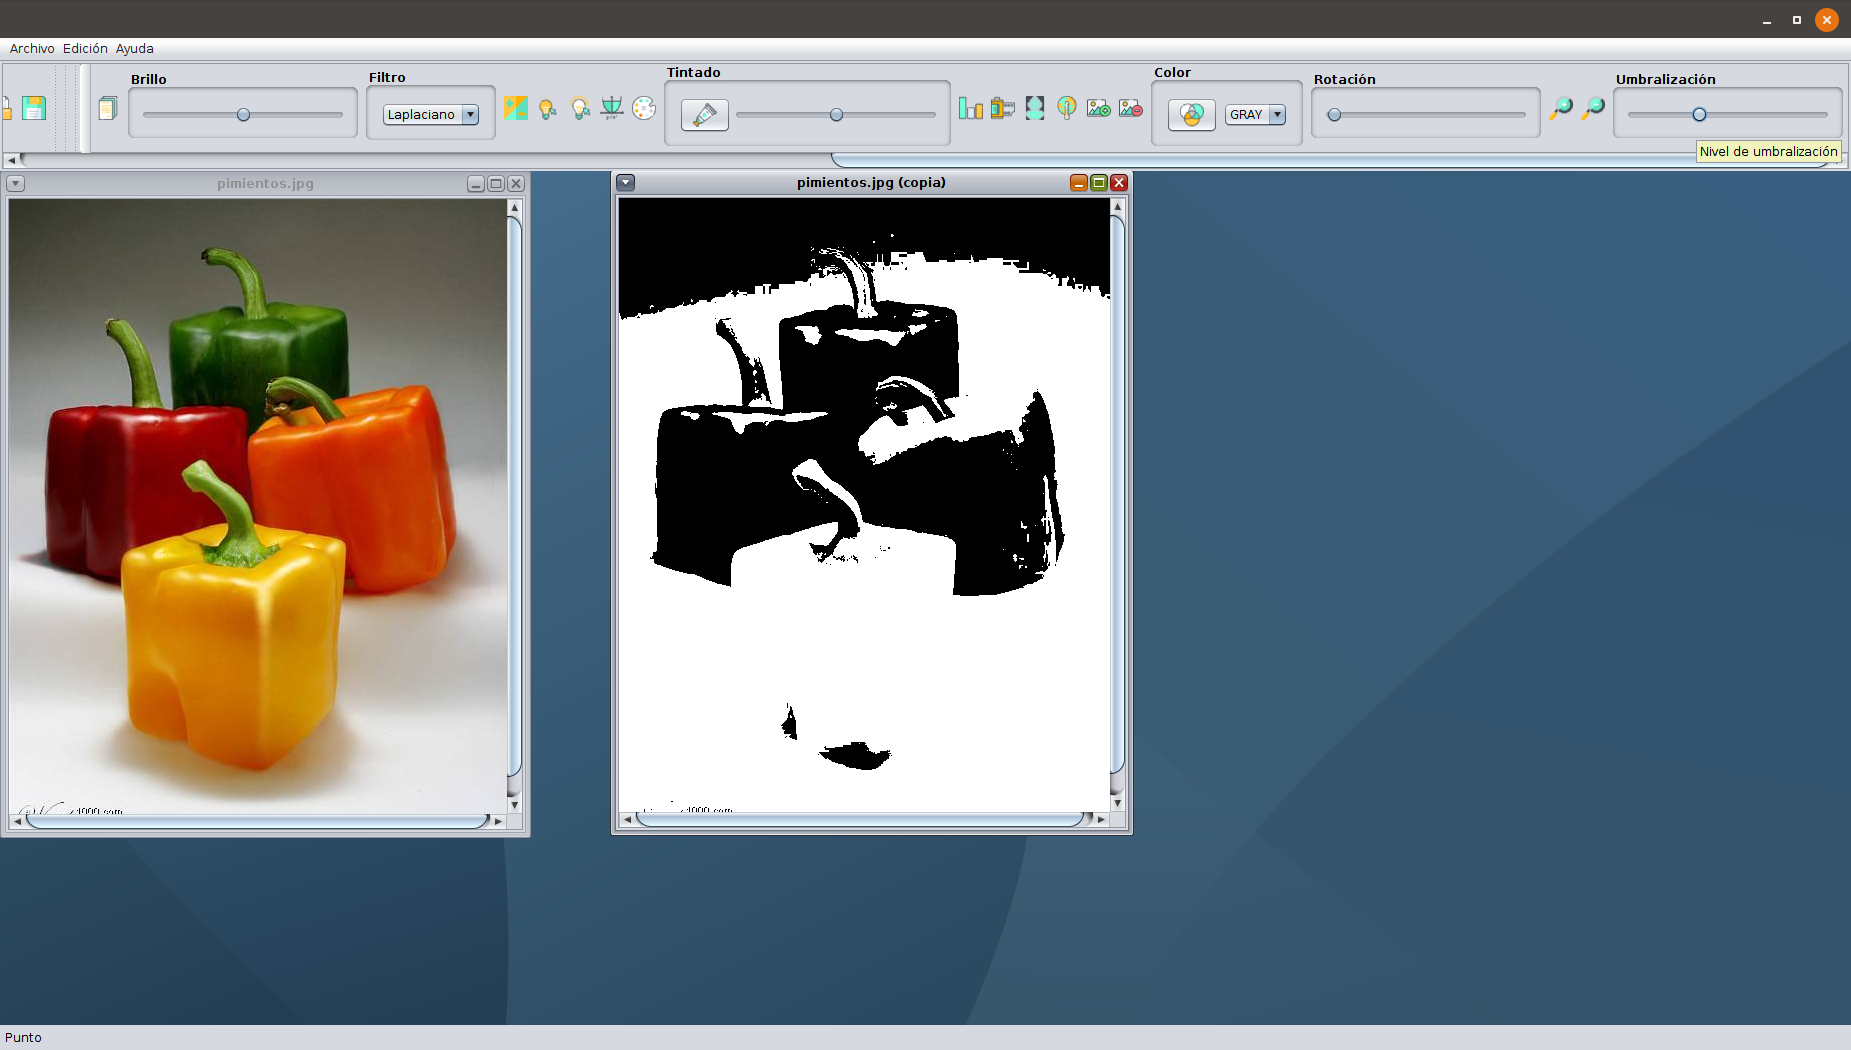
\includegraphics[width=0.6\textwidth]{img/umbral.png}
\end{figure}

\subsubsection{Función propia}
En este caso, se pide implementar una función propia. La función implementada cumple con la siguiente fórmula explícita:

\[f(x)=|x^3+|\cos(xw)|+1)|\%255\]

donde $w$ representa la velocidad angular. La representación gráfica de la función es la siguiente:

\begin{figure}[H]
\centering
	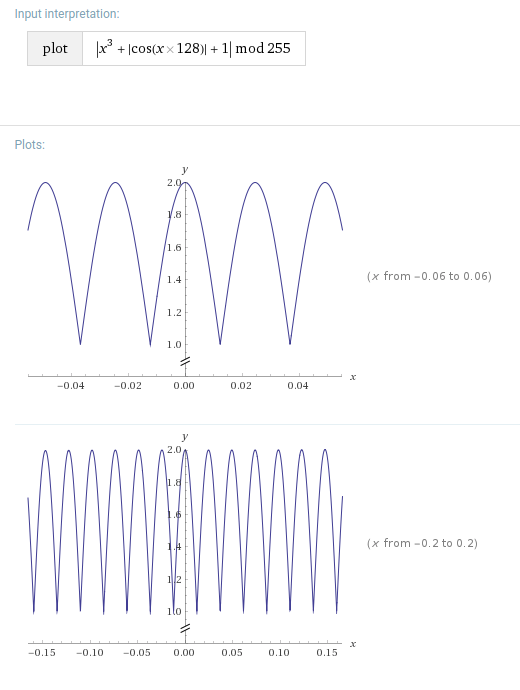
\includegraphics[width=0.5\textwidth]{img/plot.png}
\end{figure}

A pesar de que en el gráfico no sale, la función está definida entre 0 y 255.\\

El aspecto que le da a la imagen es poco convencional y difícil de entender, pues ni yo misma entiendo qué pasa con los colores que se le asignan a los pixeles. La imagen final es un tanto bizarra, pero a la vez divertida, puesto que los colores no se invierten exactamente pero distan mucho de los originales. Un ejemplo de uso es este:

\begin{figure}[H]
\centering
	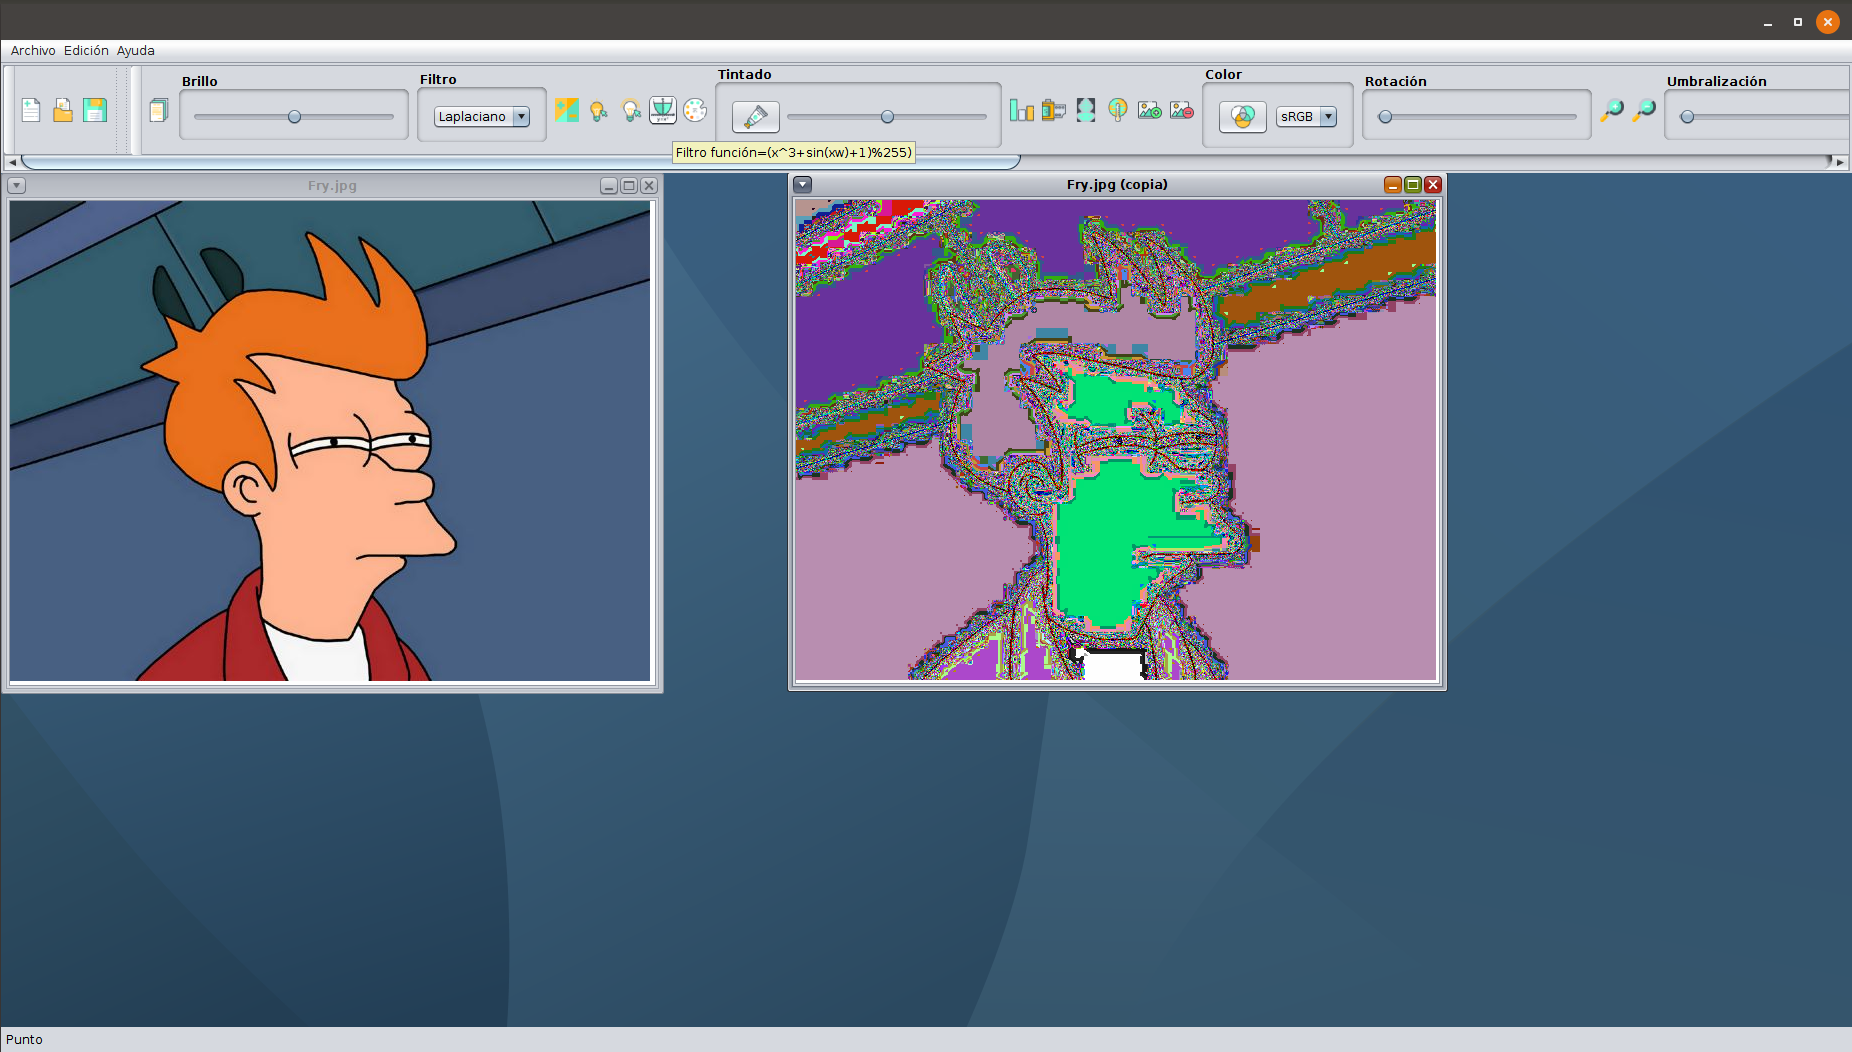
\includegraphics[width=0.6\textwidth]{img/propia.png}
\end{figure}

\subsubsection{Termal}
El filtro crea algo similar a un filtro de fronteras pero que trata los colores, es decir, en este caso, busca aquellos pixeles con tonos de rojo intenso (por encima de 128 si hablamos entre 0 y 255) y los deja igual, mientras que los demás los pone en escala de gris. De esta forma, se resaltan las partes rojas entre lo demás (por eso lo he llamado termal, ya que el rojo se asigna siempre a un color cálido).\\

Para ello, se ha definido una clase propia, TermalOp, que calcula el valor de cada pixel. Es una operación componente a componente, ya que el valor de cada componente del pixel no depende de los demás.\\

Un ejemplo de uso es el siguiente (la primera es una imagen normal, la segunda una tomada con la webcam):

\begin{figure}[H]
\centering
	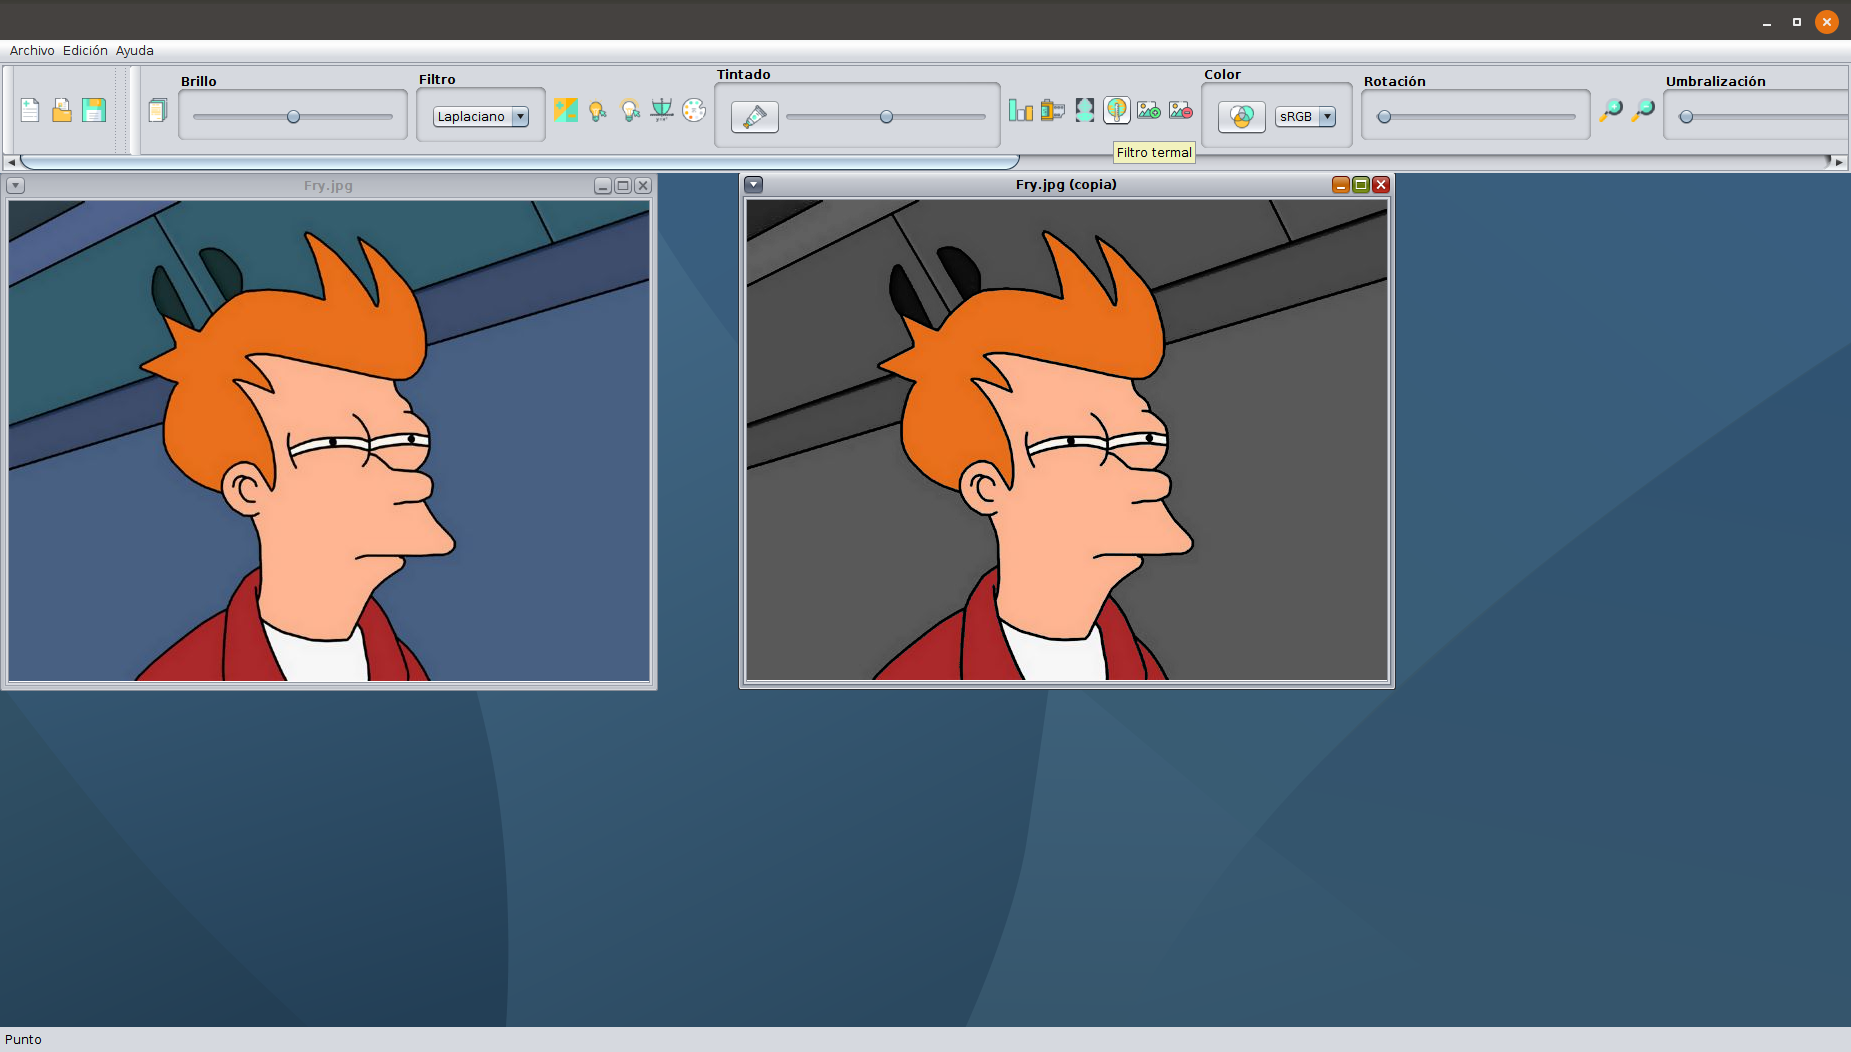
\includegraphics[width=0.6\textwidth]{img/termal.png}
\end{figure}

\begin{figure}[H]
\centering
	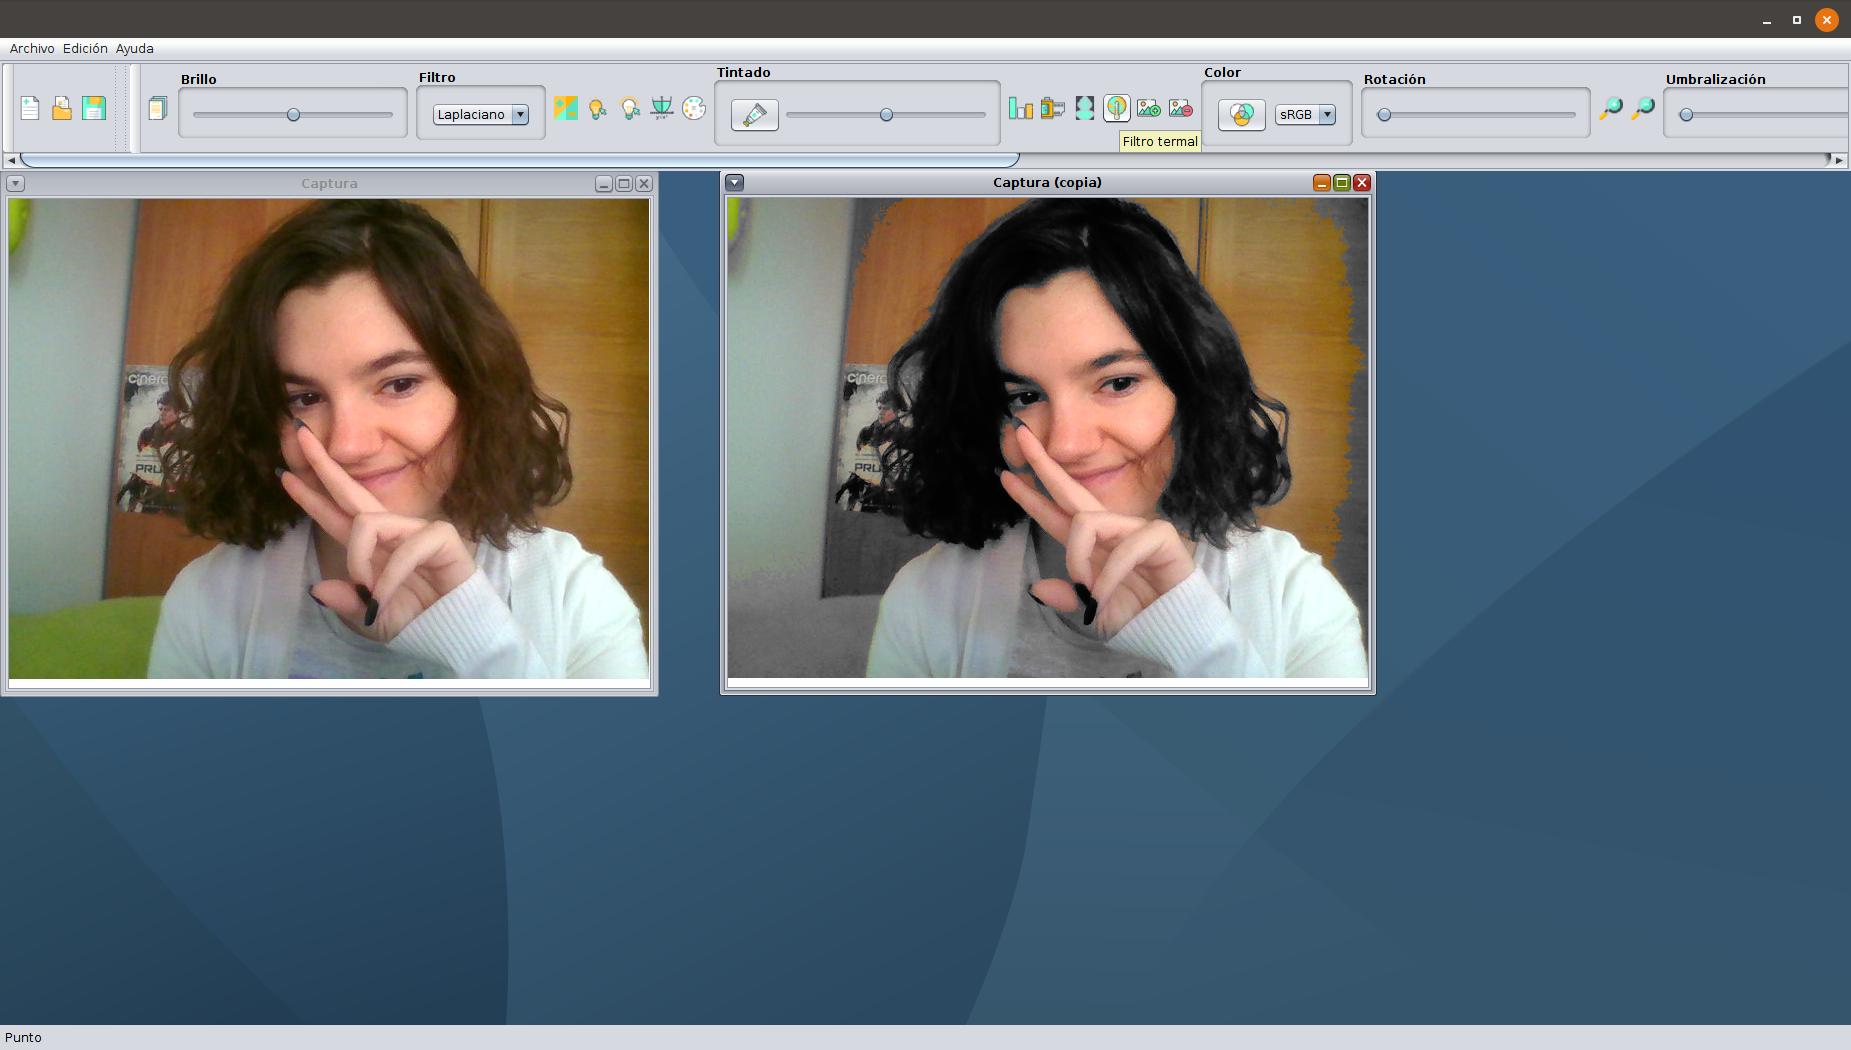
\includegraphics[width=0.6\textwidth]{img/thermal.png}
\end{figure}

Como se puede comprobar, las partes con más rojizas o anaranjadas son las que se mantienen mientras que el resto pasan a escala de gris.

\subsubsection{Rayos X}
La idea de este filtro es conseguir que las imágenes tengan los colores de una radiografía como la siguiente:

\begin{figure}[H]
\centering
	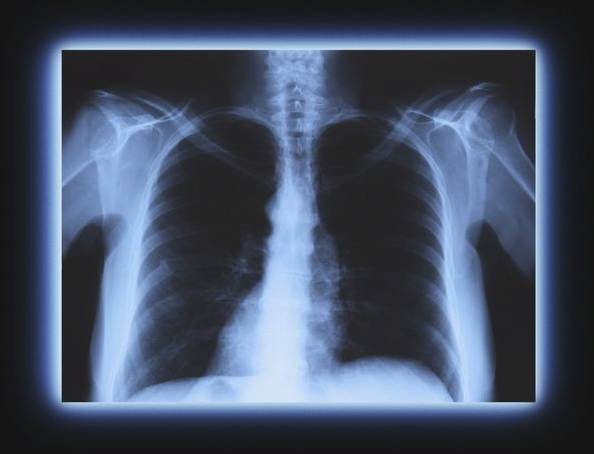
\includegraphics[width=0.4\textwidth]{img/ejemplo.png}
\end{figure}

Para ello, se ha creado una clase RayosXOp, que aplica esta operación pixel a pixel; el valor final de un pixel se calcula como la media de los tres componentes: si está por debajo del umbral inferior, es decir, si es una parte oscura, se destacará igual que ocurre con los huesos en la radiografía; si está entre el umbral inferior y el superior, tendrá una tonalidad intermedia, como se ven los músculos y piel en las radiografías; y si está por encima del umbral superior, esa zona quedará oscura, ya que no es lo que nos interesa y se tomará como información despreciable (como ocurren con el fondo de la sala en las radiografías).\\

Un ejemplo de su uso con las mismas imágenes que en el filtro termal es el siguiente:

\begin{figure}[H]
\centering
	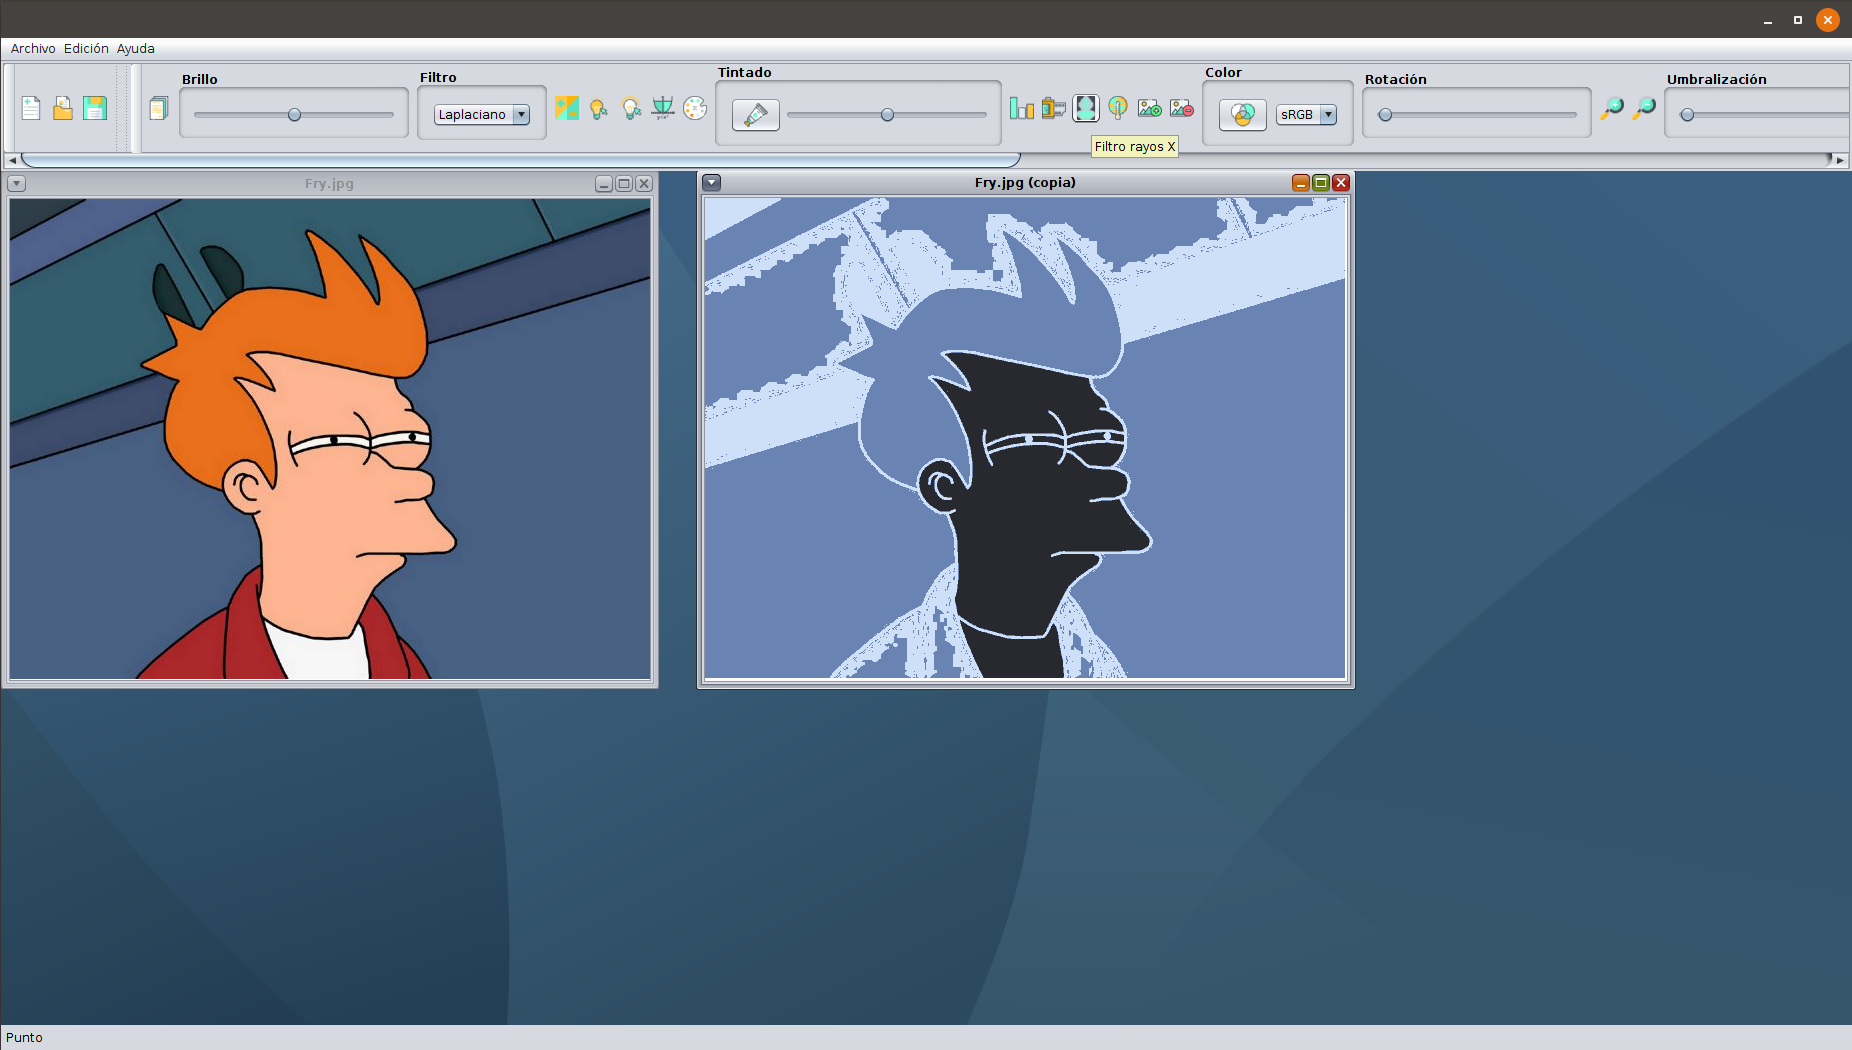
\includegraphics[width=0.6\textwidth]{img/rayosx.png}
\end{figure}

\begin{figure}[H]
\centering
	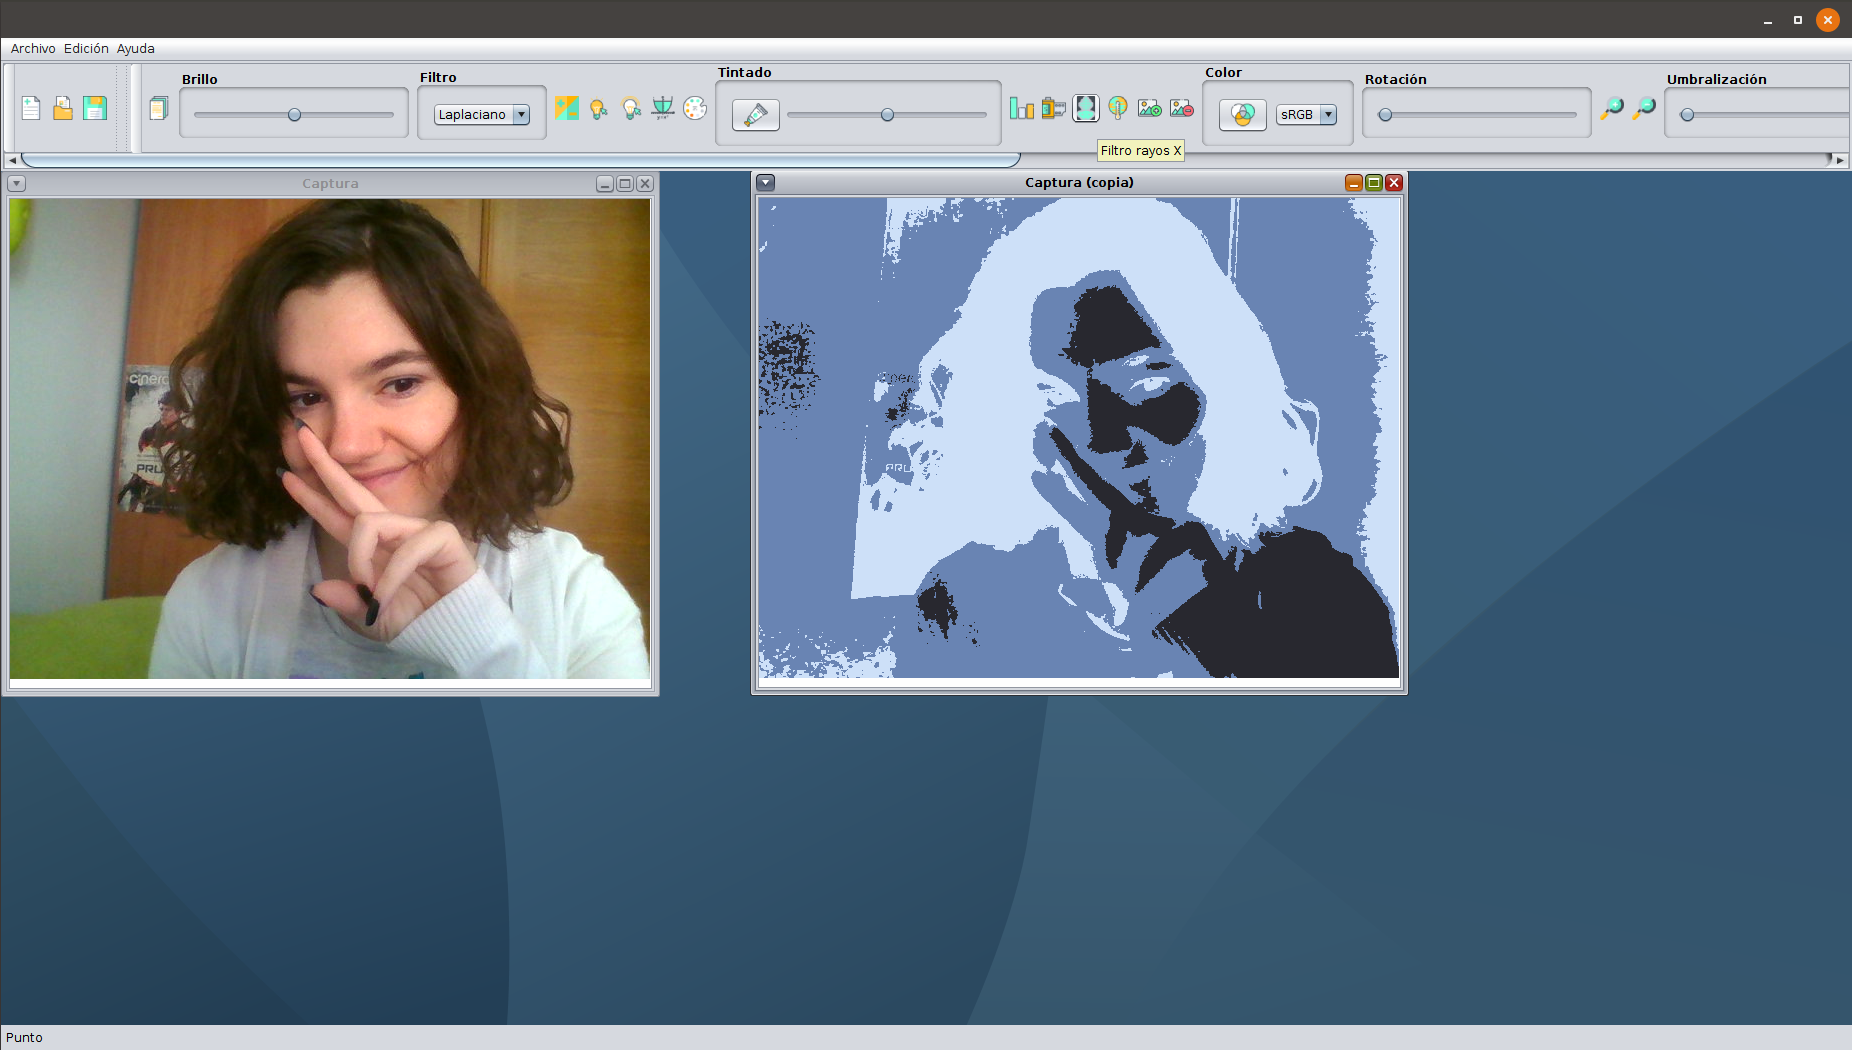
\includegraphics[width=0.6\textwidth]{img/xray.png}
\end{figure}

\subsubsection{Suma de imágenes}
En este caso, se unen dos imágenes en una, superponiendo la segunda encima de la primera, con un grado de transparencia de 0,5. La imagen generada es una nueva, que conserva las dimensiones de la primera imagen. Para poder aplicarlo, se ha utilizado la operación \textsc{BlendOp} del paquete \textsc{sm.image}.\\

Un ejemplo de uso es el siguiente:

\begin{figure}[H]
\centering
	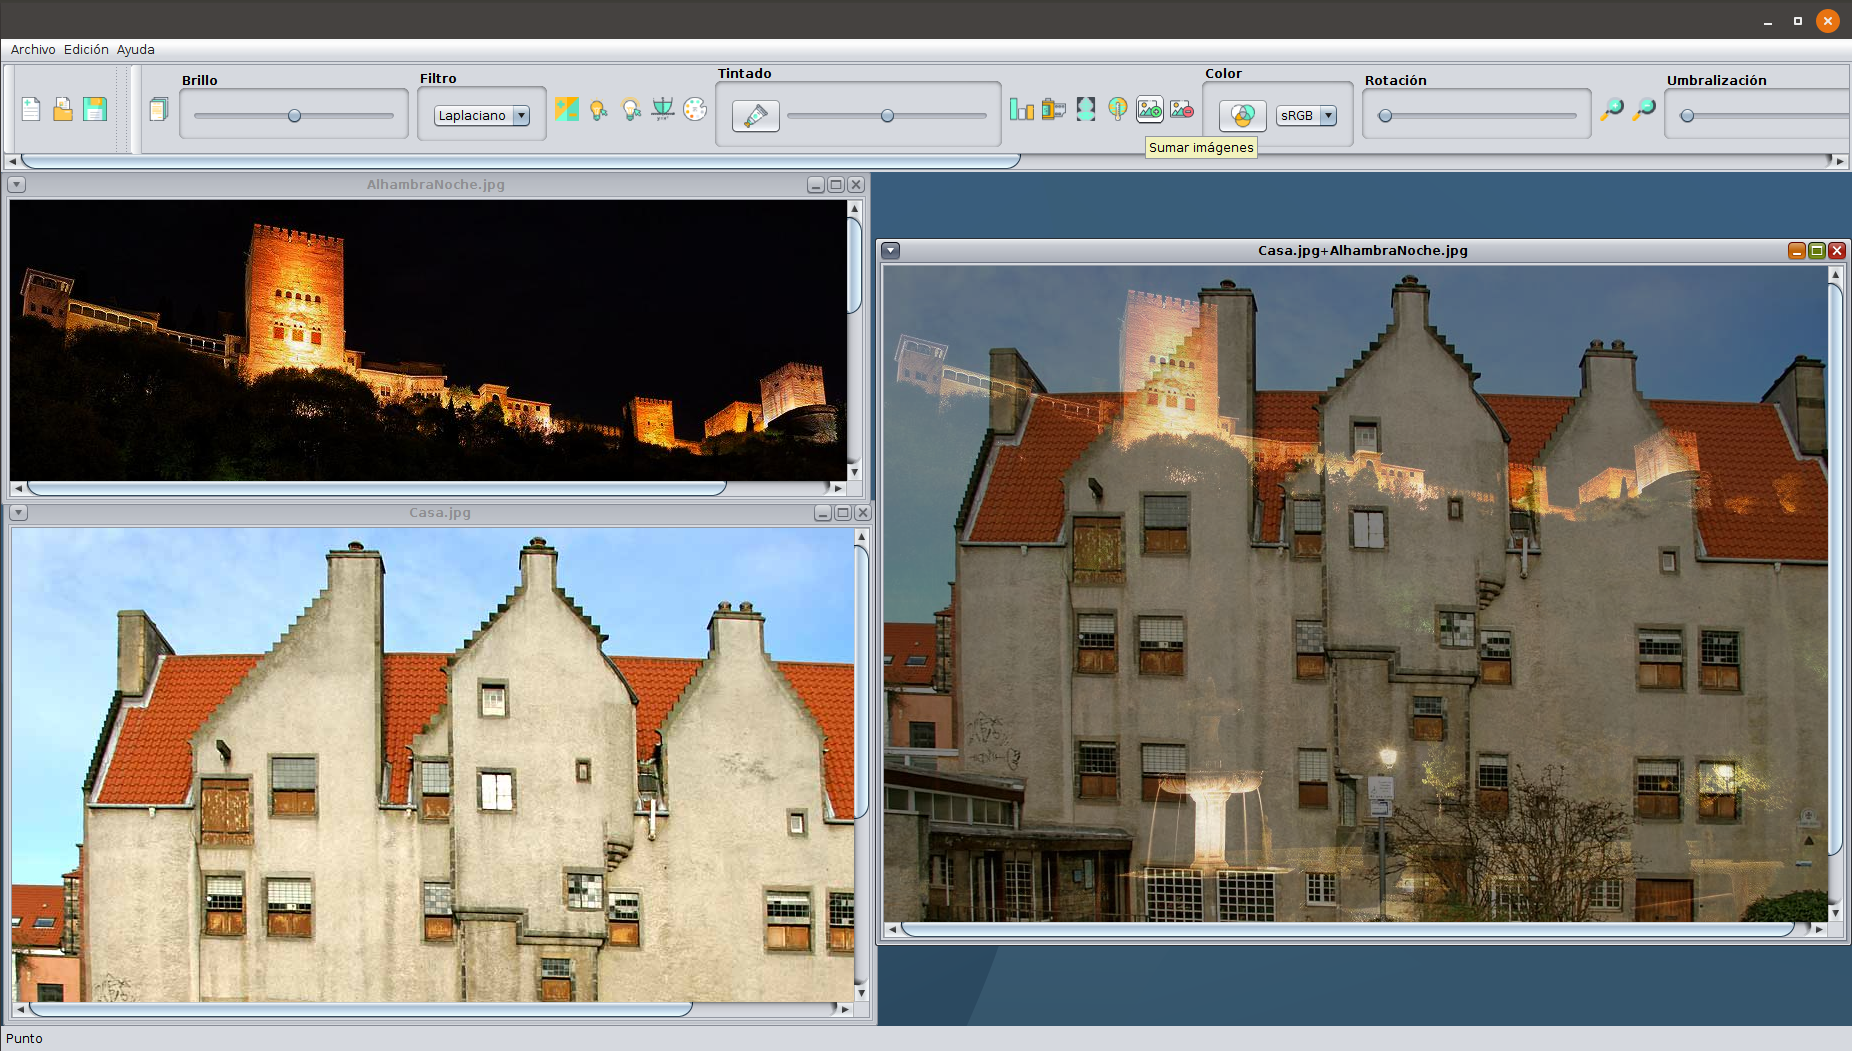
\includegraphics[width=0.6\textwidth]{img/suma.png}
\end{figure}

\subsubsection{Resta de imágenes}
Al contrario que en el caso anterior, en la resta la idea es de nuevo superponer dos imágenes, pero estando en negativo aquella que se superpone. Es decir, las partes negras pasarían a blanco al superponerla. Para que el efecto se muestre, se ha usado \textsc{SubtractionOp}, también del paquete \textsc{sm.image}.\\

Un ejemplo de uso es el que sigue:

\begin{figure}[H]
\centering
	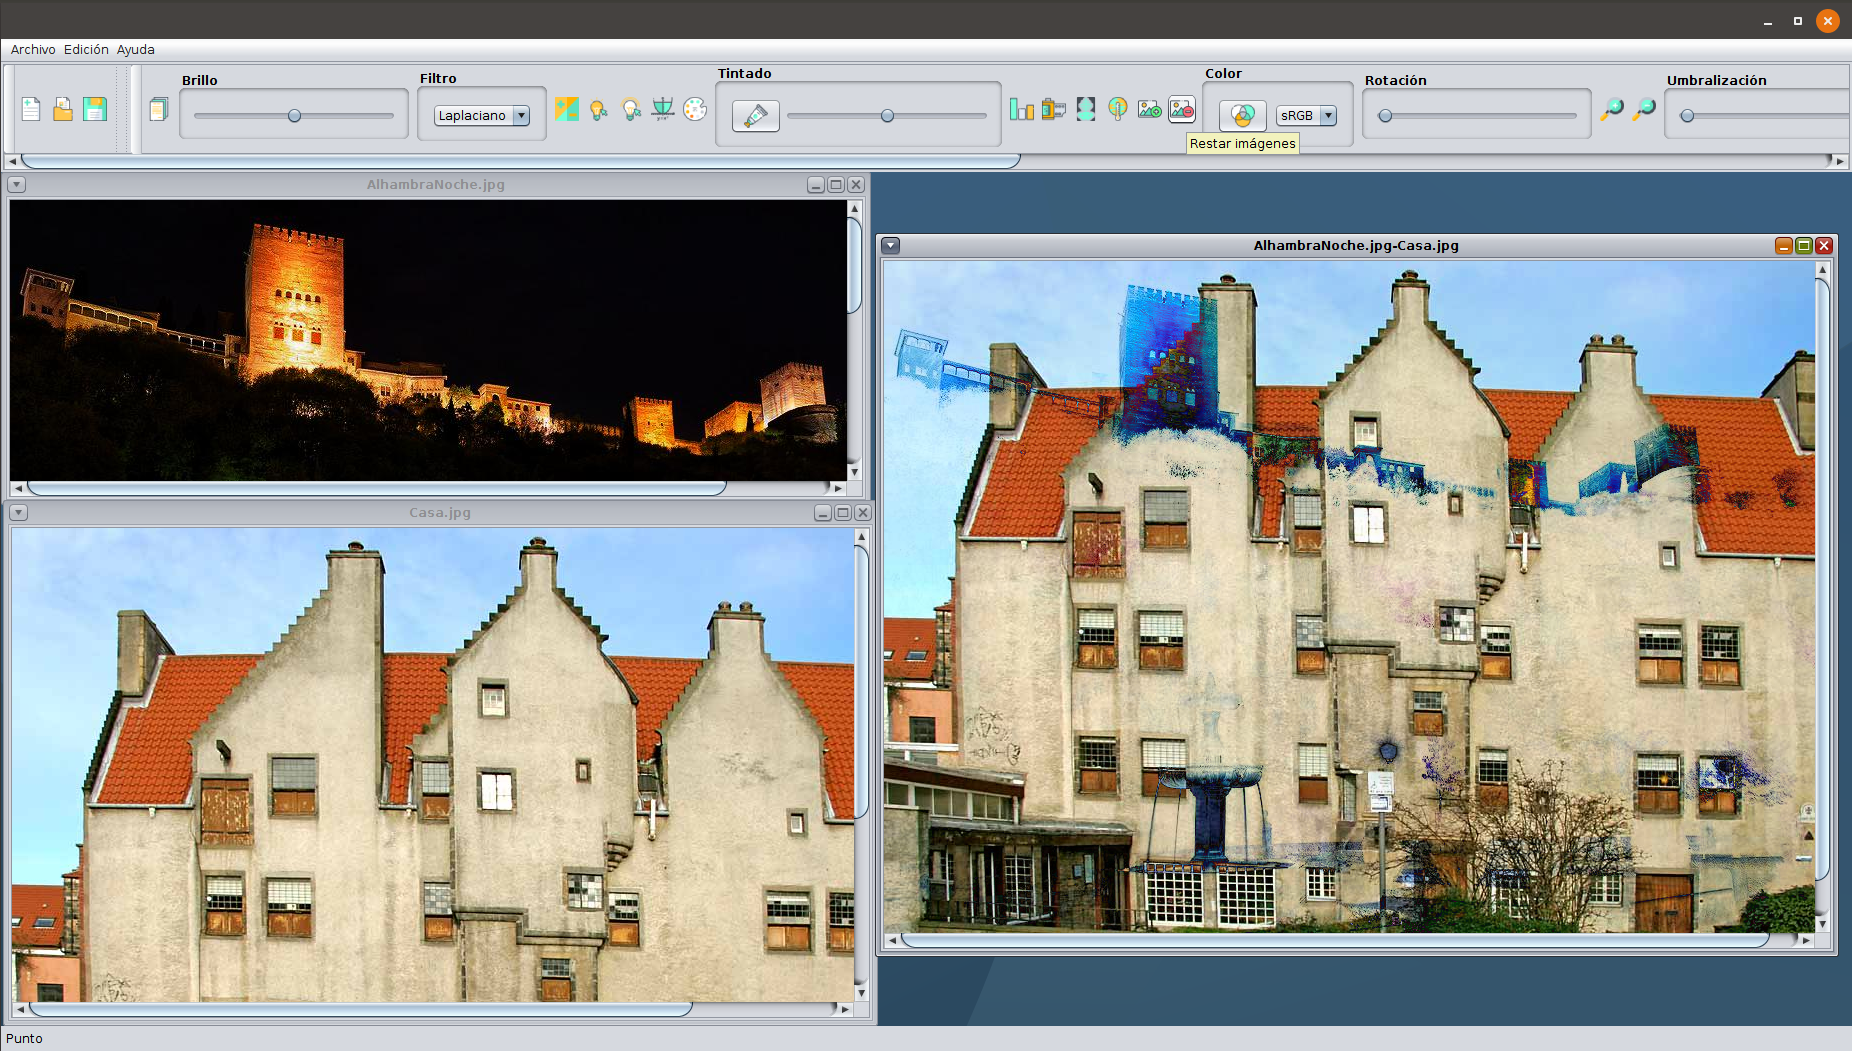
\includegraphics[width=0.6\textwidth]{img/resta.png}
\end{figure}

\subsubsection{Tintado (mediante deslizador)}
Por último, la operación de tinte aplicada al botón se aplicará también con un deslizador. La diferencia fundamental es que, en este caso, la potencia que se le da no es de 0,5 sino que es el usuario el que la elige mediante el deslizador, que va de 0 a 1, donde 0 significa que no hay tintado y 1 significa que se ha tintado la imagen completamente.\\

Para ello, se utilizará el color seleccionado, en este ejemplo (al igua que en el del botón), se ha usado el color amarillo.\\

Un ejemplo de su uso, en el que se muestra la diferencia con la imagen utilizada en la explicación del tinte con botón es la siguiente:

\begin{figure}[H]
\centering
	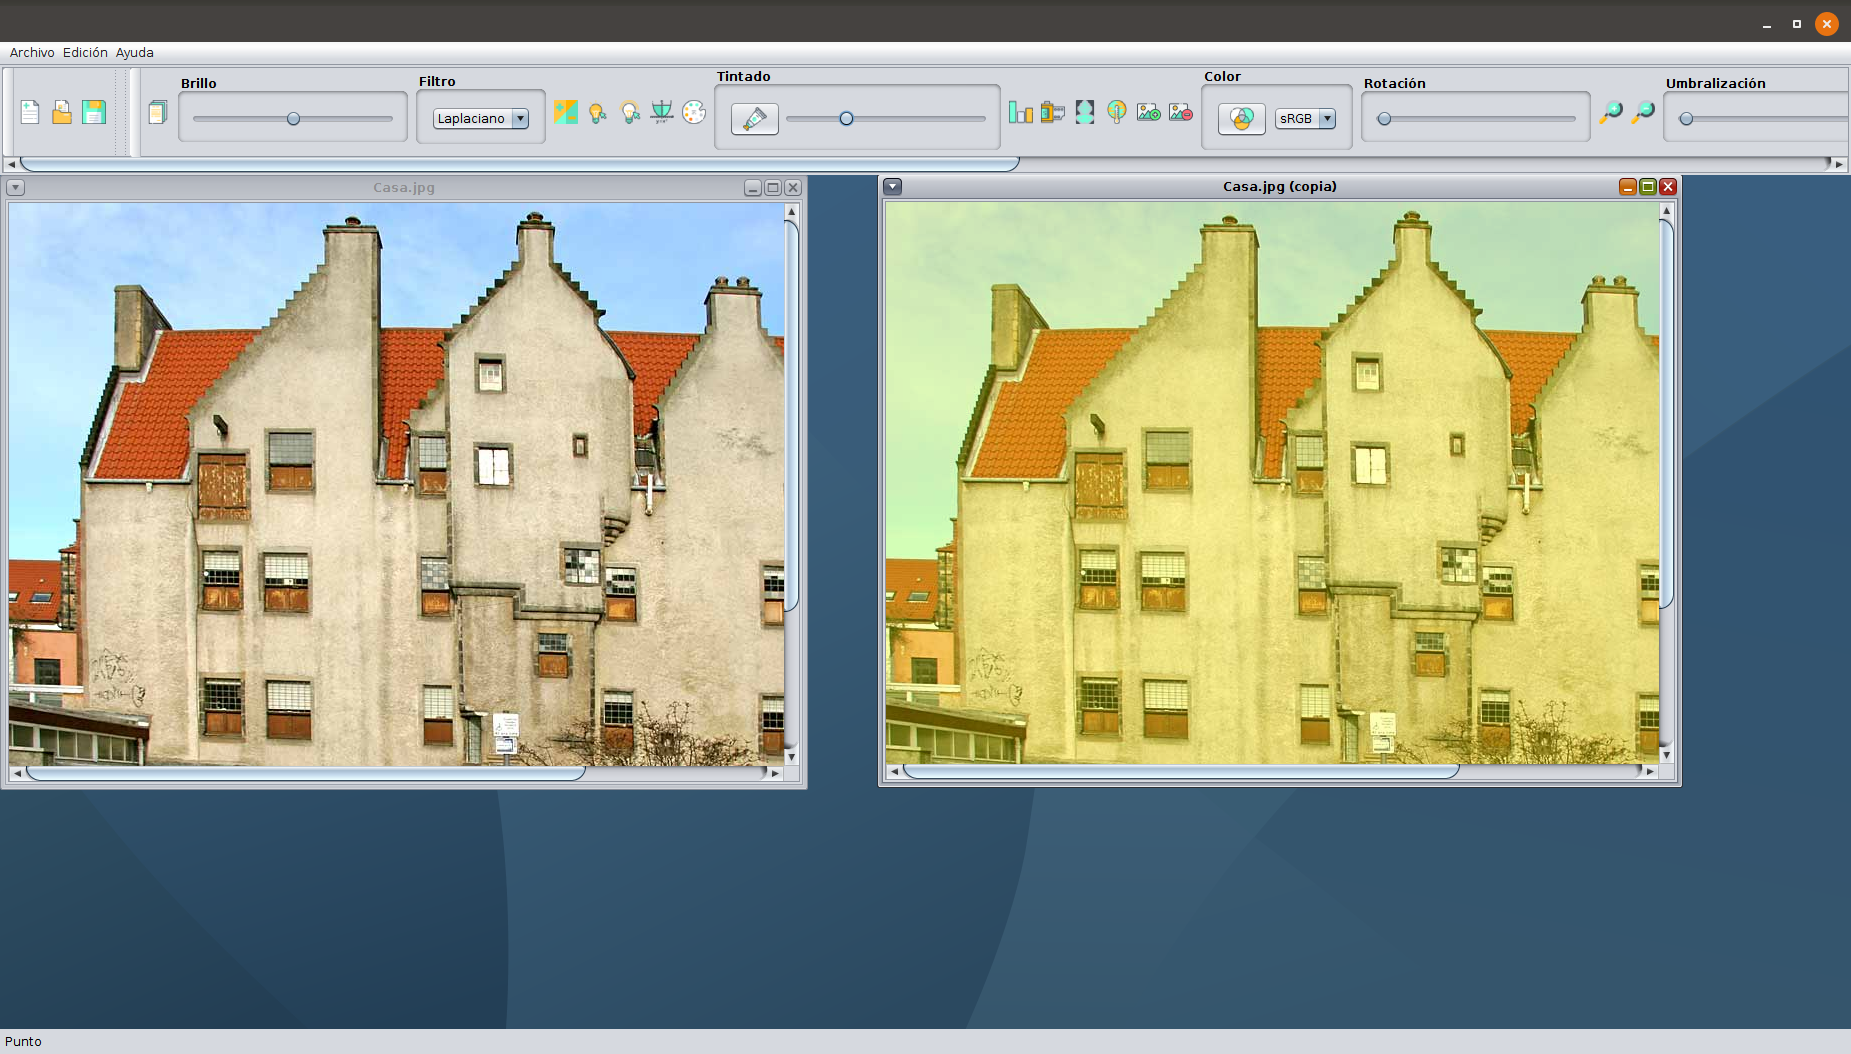
\includegraphics[width=0.6\textwidth]{img/tintedes.png}
\end{figure}

En este caso, al poder elegir, la imagen se ve mucho menos amarilla que en el caso del botón, ya que la potencia no supera el 30\%.

\newpage

\section{Sonido}

\subsection{Análisis de requisitos}
Respecto a la parte de sonido, el sistema cuenta con los siguientes requisitos:

\begin{itemize}
	\item RF1. Reproducir sonido.
	\item RF2. Grabar sonido.
	\item RF3. Incluir un temporizador de grabación.
	\item RF4. Mantener disponibles los archivos que se abran o graben en una lista.
\end{itemize}

\subsection{Explicación de cada requisito}
La explicación para cada requisito de sonido es la siguiente:

\begin{itemize}
	\item RF1. El sistema reproducirá los sonidos en los formatos \textsc{.au} y \textsc{.wav}. Para ello, se incluirá un botón de reproducción que empezará a reproducir el audio cuando se pulse; también incluirá un botón de stop que parará la canción y la reiniciará, de forma que al volver a pulsar el botón de reproducción, comenzará desde el principio. Adicionalmente, se añadirá un botón de pausa que detenga la canción pero no la rebobine, es decir, que cuando se vuelva a reproducir, lo haga desde donde se quedó.
	\item RF2. Se añadirá un grabador de voz que utilice el micrófono disponible del dispositivo para grabar sonido. Para ello, se incluirá un botón de inicio de grabación, y un botón de parada. Cuando se pulse éste último, la grabación se dentendrá y se abrirá un diálogo para guardar el archivo. Dicha grabación se añadirá a la lista de archivos reproducibles.
	\item RF3. Al lado de los botones de grabación de sonido, habrá un temporizador que indicará cuanto tiempo está durando la grabación.
	\item RF4. Habrá una lista que incluya todos los archivos disponibles, ya sea porque se han abierto o porque se han grabado. Seleccionando uno de los incluidos en la lista, se podrá reproducir o parar como un archivo más.
\end{itemize}

\subsection{Codificación}
Aquí explicaré brevemente el funcionamiento de cada requisito con imágenes de la aplicación.

\subsubsection{Reproducción}
Como se ha explicado previamente, se empezará a reproducir (o se detendrá) cuando se pulse el componente diseñado para este fin.\\

\begin{figure}[H]
\centering
	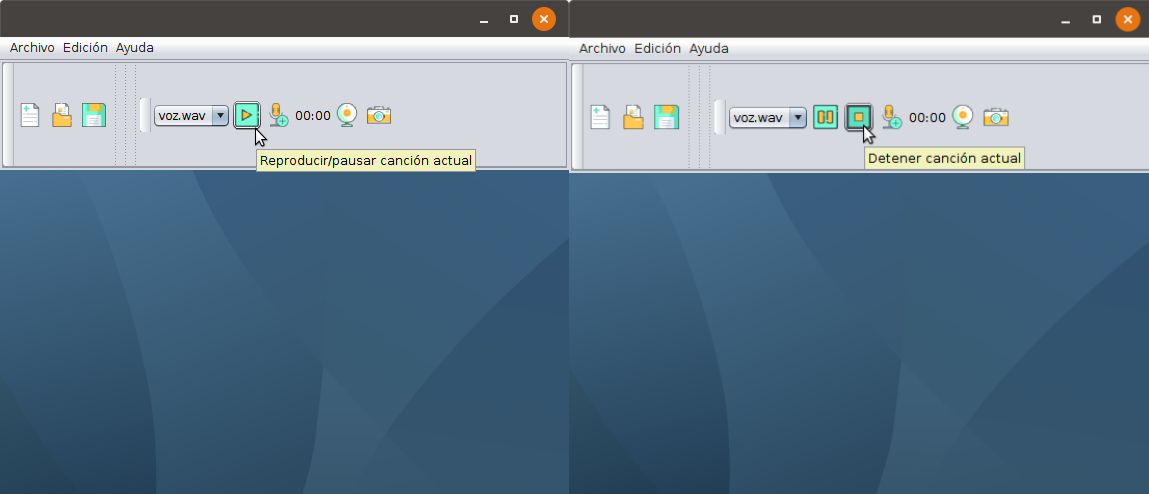
\includegraphics[width=0.7\textwidth]{img/play-stop.png}
\end{figure}

\subsubsection{Grabación y temporizador}
Referente a los requisitos RF2 y RF3, se grabará y detendrá la grabación tal y como se muestra en la imagen. Como se puede observar, mientras se está grabando, el temporizador marca los minutos y segundos que se han grabado.

\begin{figure}[H]
\centering
	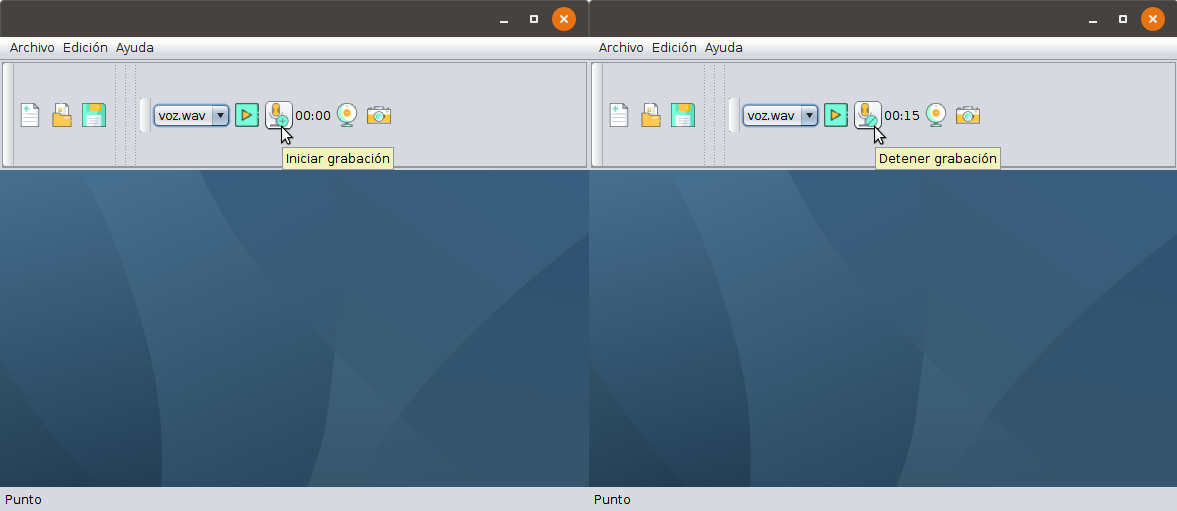
\includegraphics[width=0.7\textwidth]{img/grabacion.png}
\end{figure}

Una vez detenida la grabación, se abrirá un diálogo para guardar el archivo.

\begin{figure}[H]
\centering
	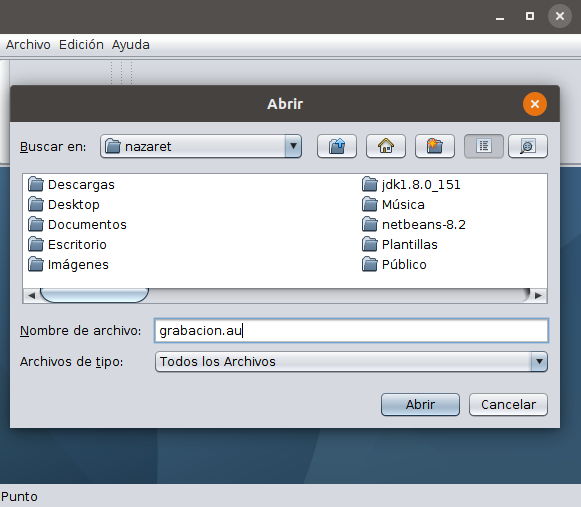
\includegraphics[width=0.35\textwidth]{img/guardar.png}
\end{figure}

\subsubsection{Lista de archivos}
Por último, se mostrará una lista (en este caso un desplegable) con los archivos que se han abierto o que se han grabado. Se podrá seleccionar el que se desee para reproducirlo.

\begin{figure}[H]
\centering
	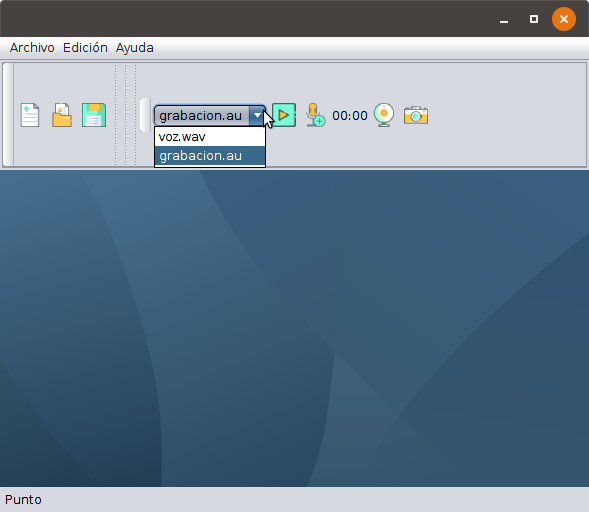
\includegraphics[width=0.5\textwidth]{img/lista.png}
\end{figure}

La lista se hará tan larga como archivos se hayan añadido.

\newpage

\section{Vídeo}

\subsection{Análisis de requisitos}
Por último, los requisitos respecto a vídeo que pide la evaluación son los que siguen:

\begin{itemize}
	\item RF1. Reproducir pistas de vídeo.
	\item RF2. Apertura de la webcam.
	\item RF3. Captura de imágenes de la webcam o de vídeo.
\end{itemize}

\subsection{Explicación de cada requisito}

\begin{itemize}
	\item RF1. Se abrirán pistas de audio en todos los formatos soportados por VLC \footnotemark .
	\item RF2. Se podrá activar la cámara conectada al dispositivo y ver en tiempo real lo que sucede.
	\item RF3. Con un botón se podrá tomar captura del vídeo (o de la cámara, según la ventana que haya seleccionada en ese momento) y se podrá procesar la imagen como si fuera una imagen cualquiera. Todas las operaciones disponibles para el resto de imágenes lo estarán para cada captura que tomemos.
\end{itemize}

\subsection{Codificación}
En este apartado explicaré el funcionamiento mediante capturas y parte de la implementación que he llevado a cabo.

\subsubsection{Reproducción}
Para poder reproducir vídeo, ha sido necesario crear un nuevo tipo de ventana interna al panel, que se dedique solo a reproducir vídeo y donde no se puedan llevar a cabo acciones como dibujar o procesar imágenes.\\

Este tipo de ventana solo se utilizará para esto, y consta de un área de visualización dada por el propio gestor de vídeo que se usa, perteneciente a la librería \textsc{vlcj}.\\

Visualmente, la reproducción será como la que sigue: se abrirá una ventana que mostrará el vídeo (primera imagen), y habrá que darle a reproducir cuando se quiera comenzar a verlo y a parar cuando se desee dejar de reproducirlo (segunda imagen).

\begin{figure}[H]
\centering
	\includegraphics[width=0.7\textwidth]{img/initvid.png}
\end{figure}

\begin{figure}[H]
\centering
	\includegraphics[width=0.7\textwidth]{img/video.png}
\end{figure}

\footnotetext{Imprescindible tener instalado el reproductor y las librerías de VLC puesto que sin ellas, la parte de vídeo no funciona.}

\subsubsection{Uso de la cámara y capturas}
De nuevo, al igual que en el caso anterior hace falta una ventana específica para la cámara del dispositivo, ya que en ese caso, además de restringirse el dibujado de formas o el procesado de imágenes, tampoco se puede parar y reanudar un archivo, ya que lo que capta la cámara es en tiempo real.\\

Para ello, se crea una ventana interna en cuyo interior se encuentra el área visual donde se mostrará la secuencia que capte el dispositivo.\\

Una vez se visualice el contenido, se podrán tomar tantas capturas como se deseen, que se guardarán en una ventana interna donde, esta vez sí, se podrá dibuja o procesar la imagen con los distintos filtros.\\

Su funcionamiento es el siguiente:\\

\begin{figure}[H]
\centering
	\includegraphics[width=0.7\textwidth]{img/webcam.png}
\end{figure}

\begin{figure}[H]
\centering
	\includegraphics[width=0.7\textwidth]{img/captura.png}
\end{figure}

\newpage

\section{Bibliografía y fuentes de código}
\begin{itemize}
	\item Transparencias de teoría y prácticas de la asignatura Sistemas Multimedia.
	\item \textcolor{blue}{\url{https://docs.oracle.com/javase/7/docs/api/java/}}
	\item \textcolor{blue}{\url{https://stackoverflow.com/}}
	\item \textcolor{blue}{\url{https://www.flaticon.com/}}
\end{itemize}

\end{document}